\subsection{FOUR-SHIP}
\label{subsec:supp_fig:form:4ship}

\paragraph{Fingertip}
\textbf{Standard formation}
--- wingman align wingtip missile rail with canopy

\textbf{Disadvantage} --- wingmen must constantly reference lead

\hfill\textbf{Reference \cref{fig:supp_fig:form:fingertip}}

\paragraph{Finger Four} 
\textbf{Loose fingertip} --- spacing now 0.2-0.3 nm,

\hfill\textbf{Reference \cref{fig:supp_fig:form:fingerfour}}

\paragraph{Route}
\textbf{Enlarged fingertip}
--- allows more heads-down time for wingmen

\hfill\textbf{Reference \cref{fig:supp_fig:form:route}}

\paragraph{Echelon \break Left / Right}
\textbf{For overhead approach \& tanker ops}
--- wingman form up similar to fingertip but all to one side

\hfill\textbf{Reference \cref{fig:supp_fig:form:echelonright}}

\begin{figure}[htbp]
    \centering
    \begin{minipage}[b]{0.5\textwidth}
        \centering
        \begin{tikzpicture}[figstyle]
            
            \coordinate (1) at (0,0);
            \coordinate (2) at ($(1)+(225:10)$);
            \coordinate (3) at ($(1)+(-45:10)$);
            \coordinate (4) at ($(3)+(-45:10)$);

            \node[yshift=-2mm] (1fig) at (1) {
                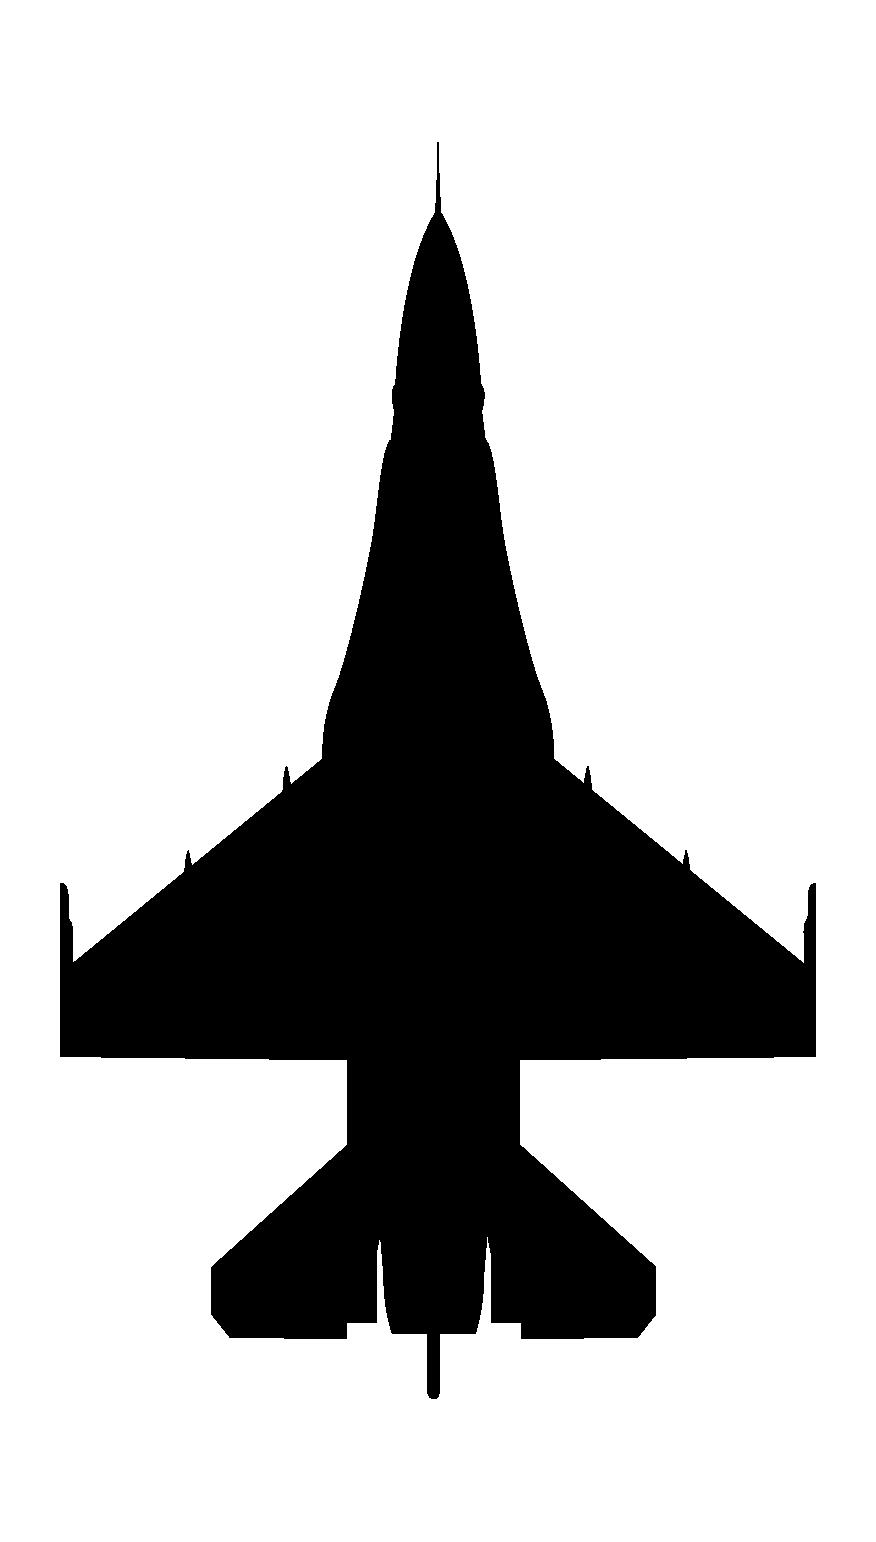
\includegraphics[
                    width=7.5mm,
                ]{diagrams/aircraft/silhouette_f16_top.pdf}
            };
            
            \node[yshift=-2mm] (2fig) at (2) {
                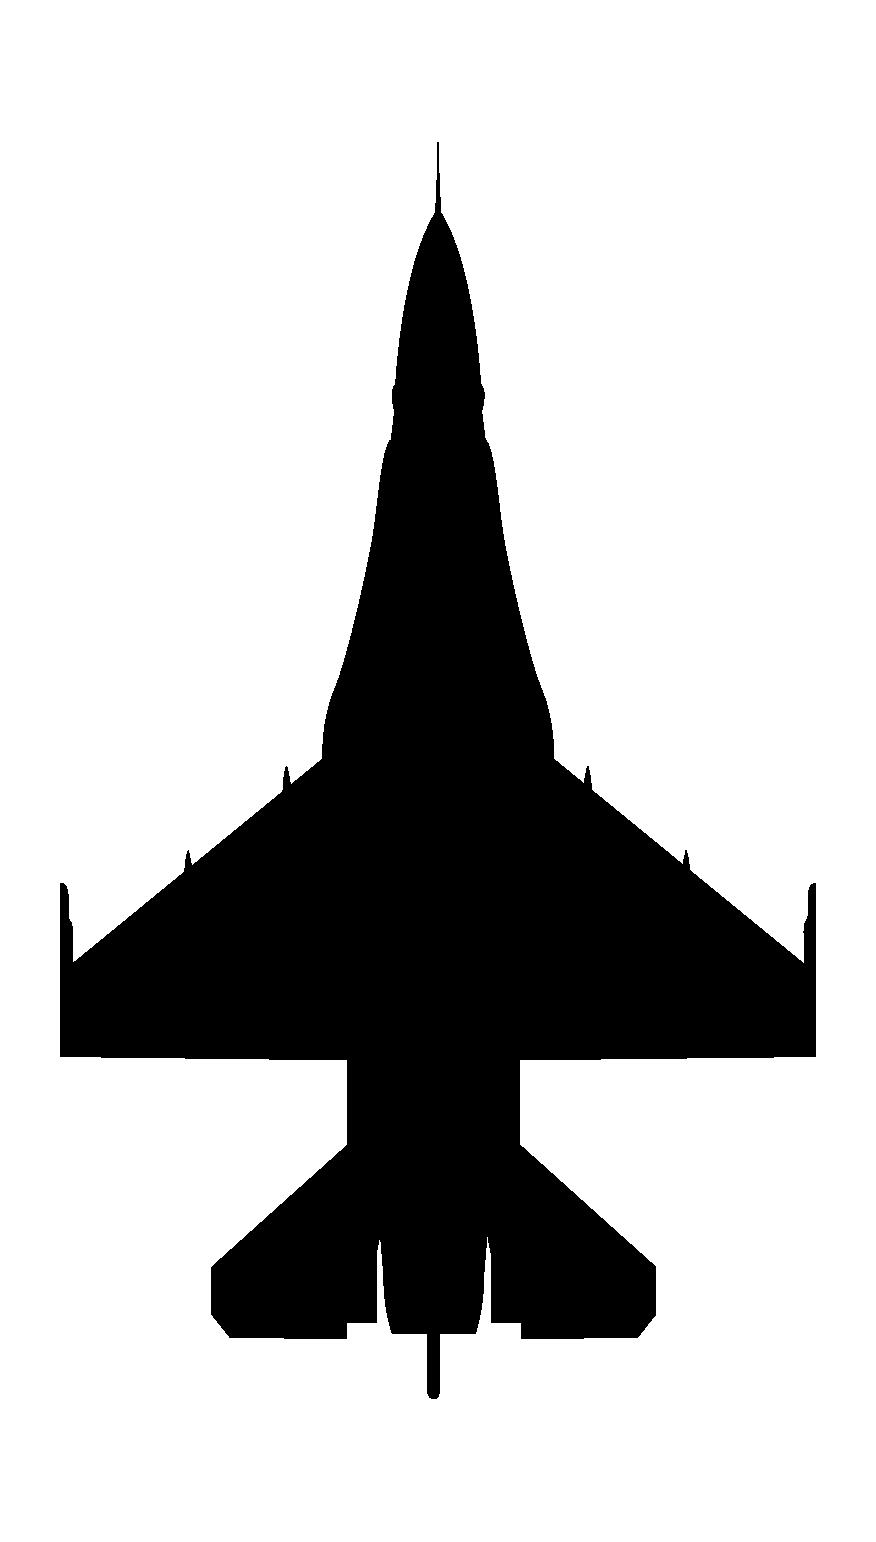
\includegraphics[
                    width=7.5mm,
                ]{diagrams/aircraft/silhouette_f16_top.pdf}
            };

            \node[yshift=-2mm] (3fig) at (3) {
                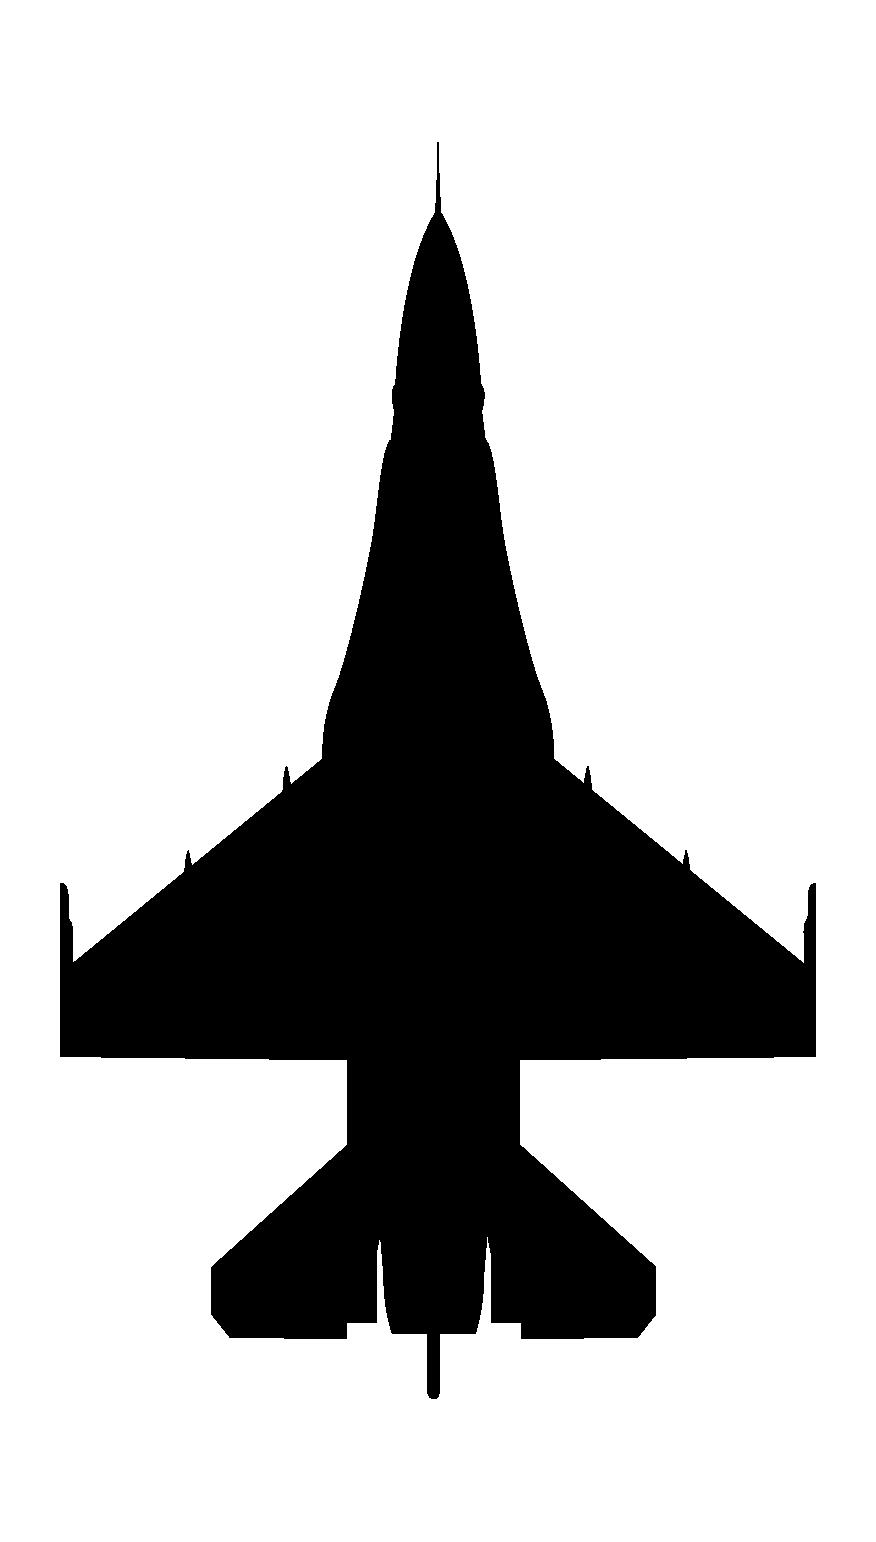
\includegraphics[
                    width=7.5mm,
                ]{diagrams/aircraft/silhouette_f16_top.pdf}
            };
            
            \node[yshift=-2mm] (4fig) at (4) {
                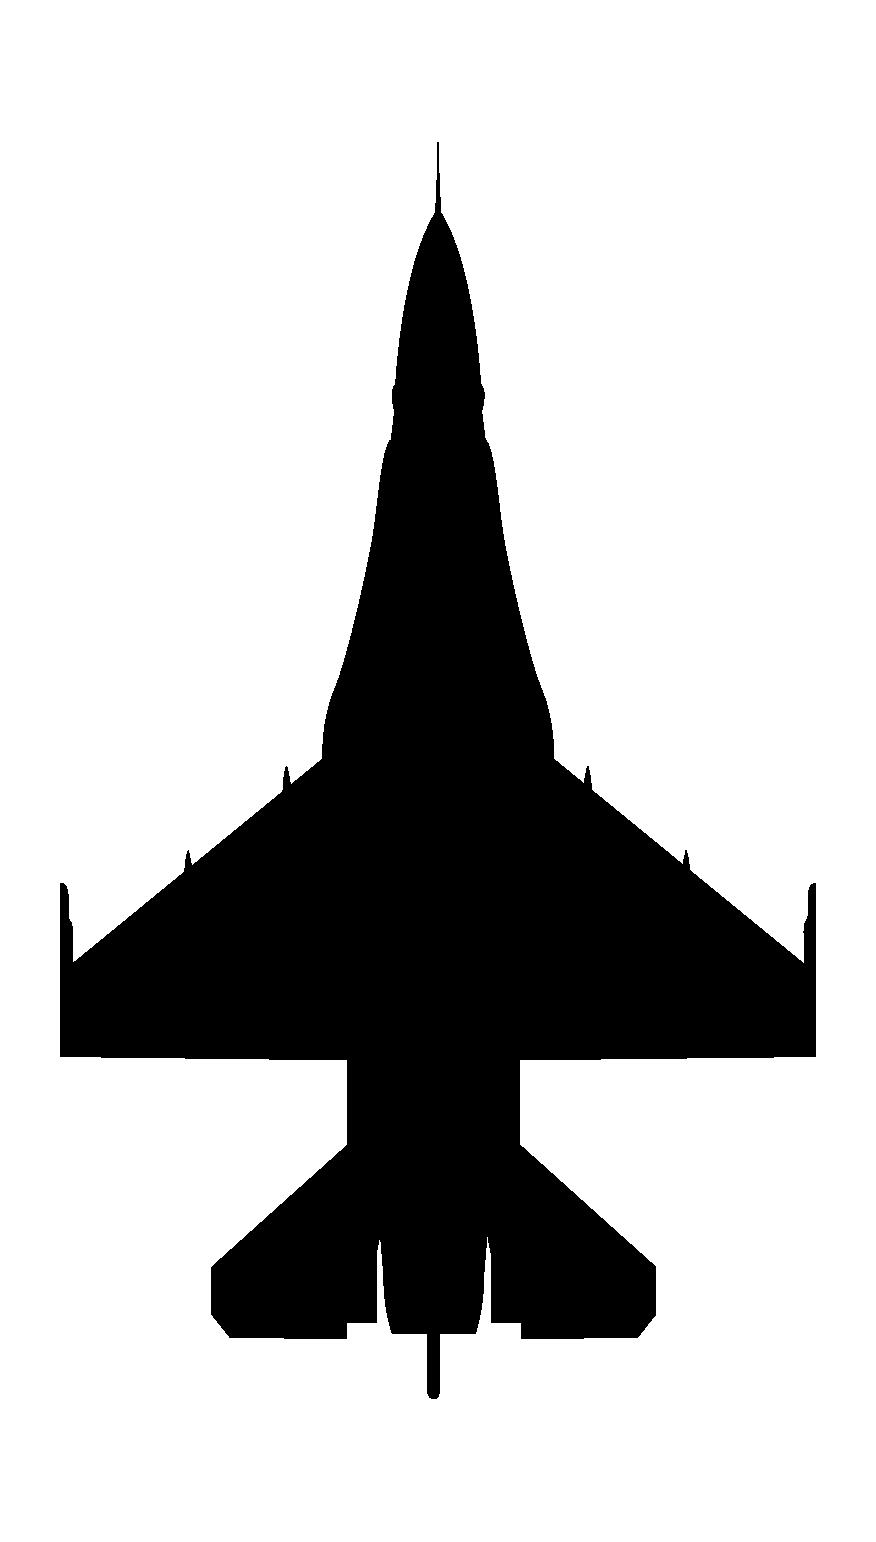
\includegraphics[
                    width=7.5mm,
                ]{diagrams/aircraft/silhouette_f16_top.pdf}
            };

            \node[anchor=north, font=\footnotesize] (1label) at (1fig.south) {1};
            \node[anchor=north, font=\footnotesize] (2label) at (2fig.south) {2};
            \node[anchor=north, font=\footnotesize] (3label) at (3fig.south) {3};
            \node[anchor=north, font=\footnotesize] (4label) at (4fig.south) {4};

        \end{tikzpicture}
        \caption{Fingertip}
        \label{fig:supp_fig:form:fingertip}
    \end{minipage}%
    \begin{minipage}[b]{0.5\textwidth}
        \centering
        \begin{tikzpicture}[figstyle]
            
            \coordinate (1) at (0,0);
            \coordinate (2) at ($(1)+(210:15)$);
            \coordinate (3) at ($(1)+(-30:15)$);
            \coordinate (4) at ($(3)+(-30:15)$);

            \draw[]
            (1) -- (2) 
            node[font=\footnotesize, above, pos=0.5, rotate=30] {0.3 nm}
            (1) -- (3) 
            node[font=\footnotesize, above, pos=0.5, rotate=-30] {0.3 nm}
            (3) -- (4)
            node[font=\footnotesize, above, pos=0.5, rotate=-30] {0.3 nm};

            \node[yshift=-2mm] (1fig) at (1) {
                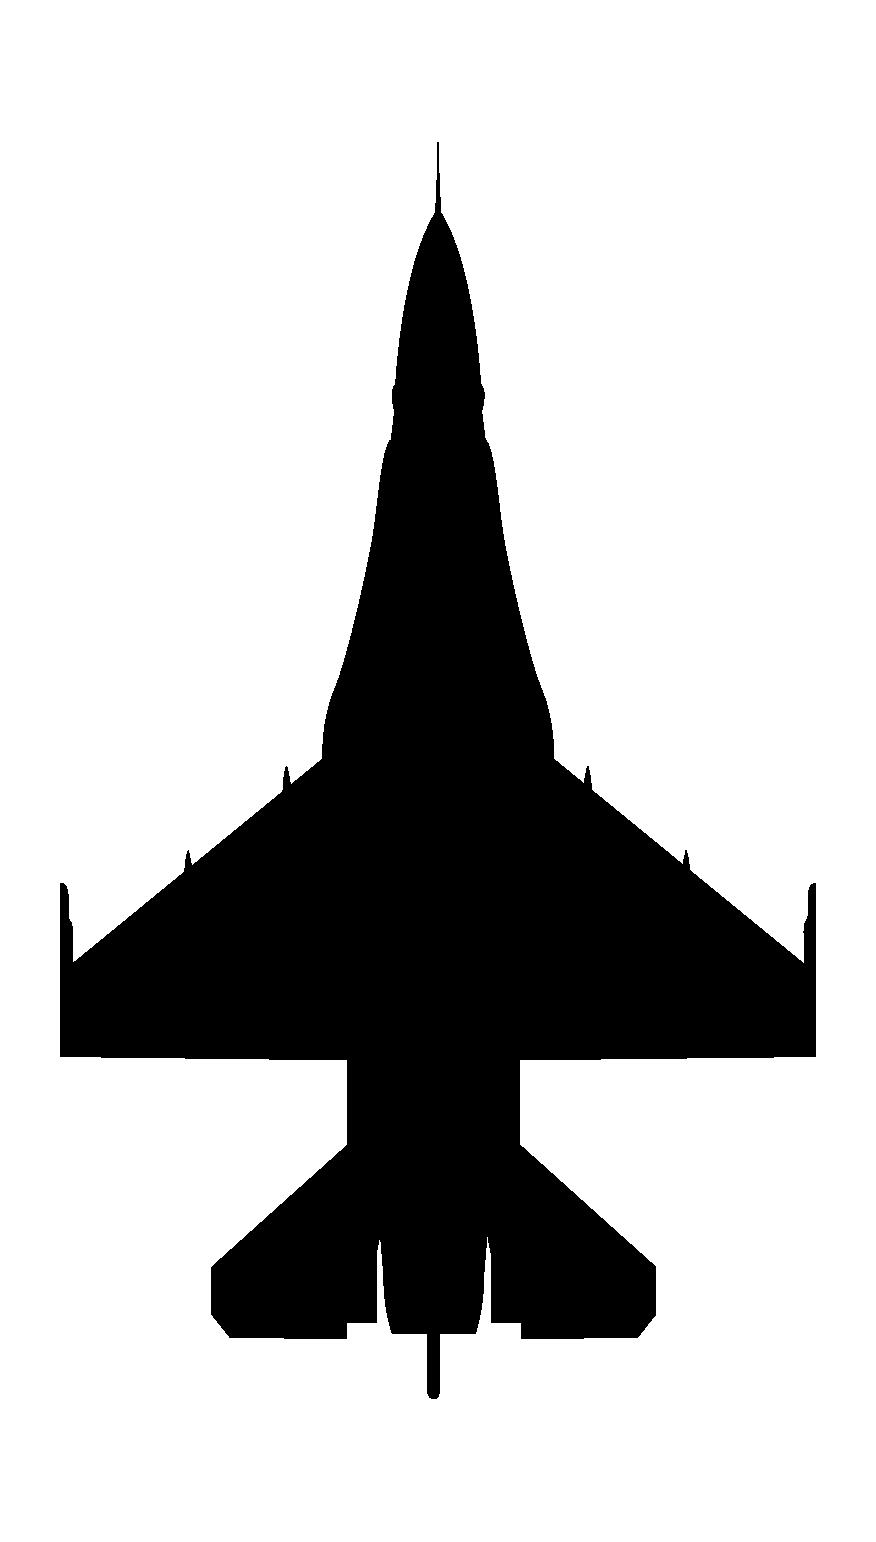
\includegraphics[
                    width=7.5mm,
                ]{diagrams/aircraft/silhouette_f16_top.pdf}
            };
            
            \node[yshift=-2mm] (2fig) at (2) {
                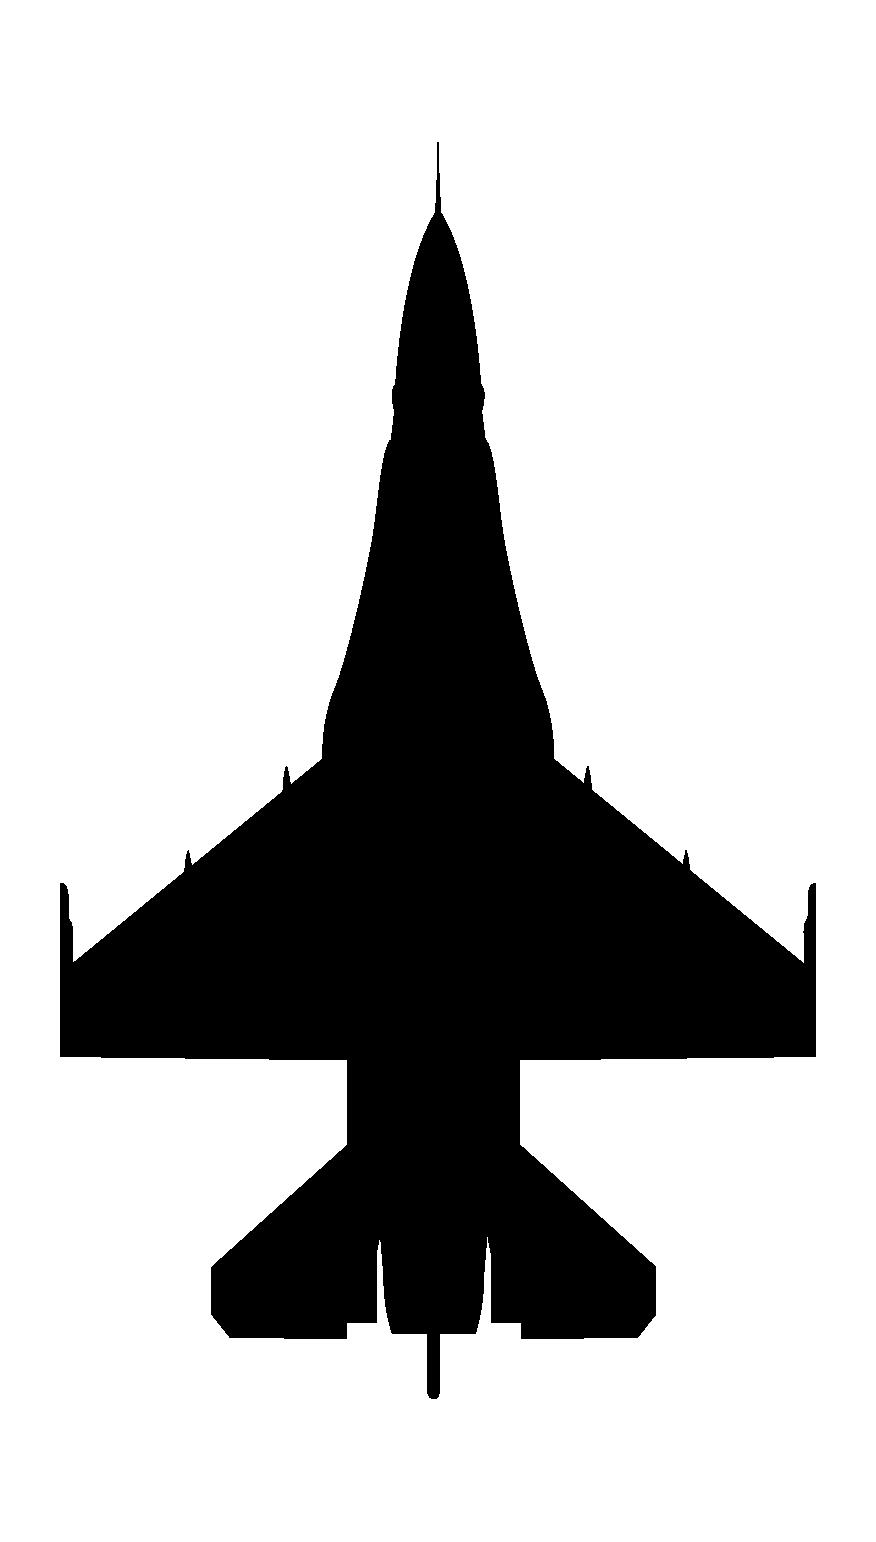
\includegraphics[
                    width=7.5mm,
                ]{diagrams/aircraft/silhouette_f16_top.pdf}
            };

            \node[yshift=-2mm] (3fig) at (3) {
                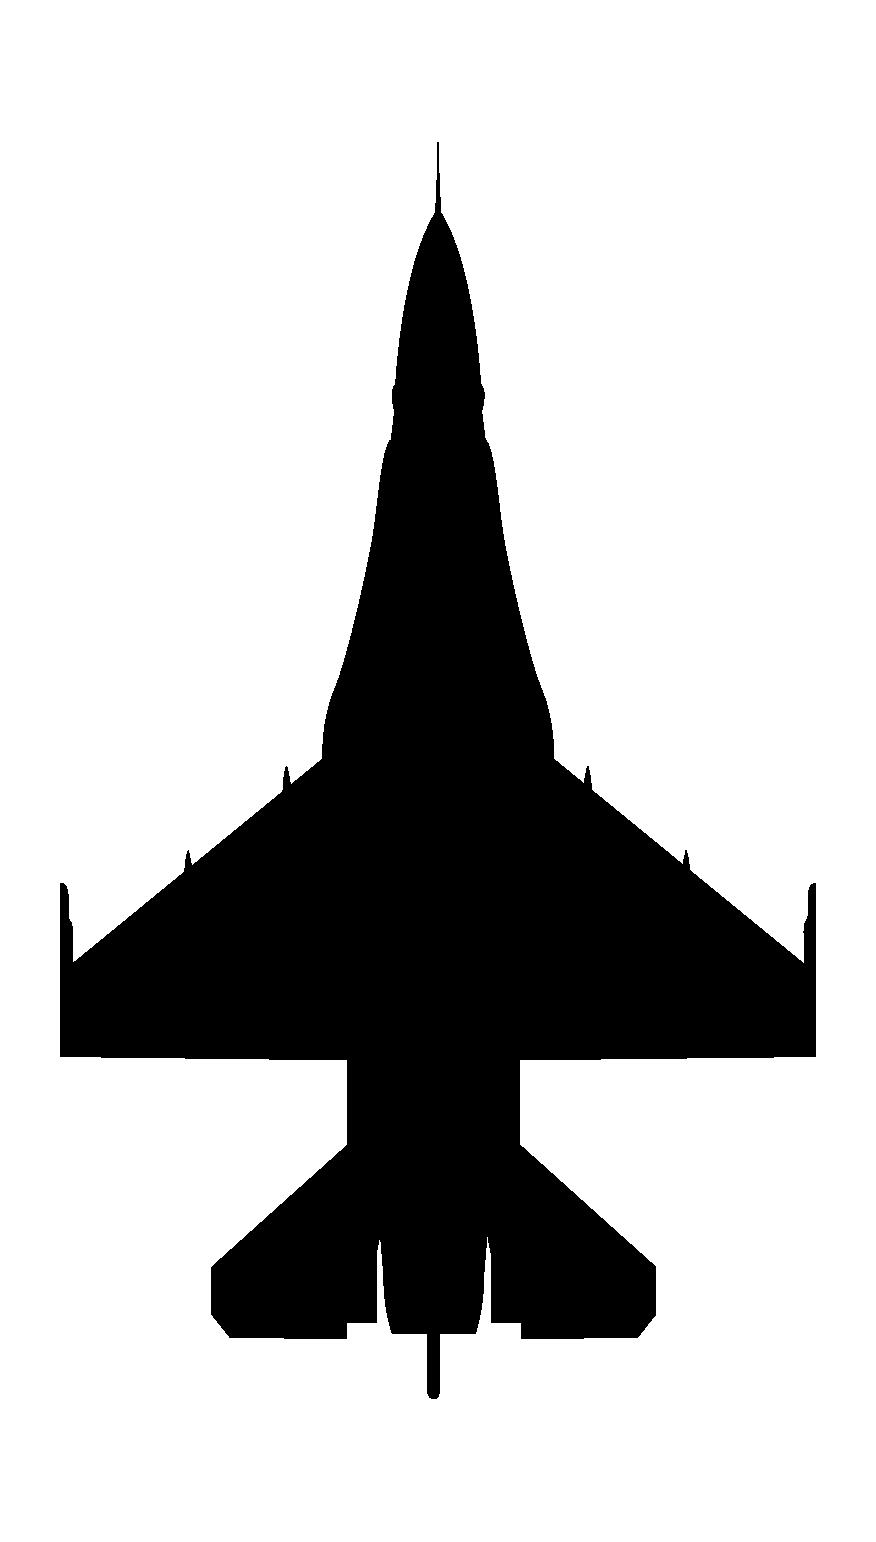
\includegraphics[
                    width=7.5mm,
                ]{diagrams/aircraft/silhouette_f16_top.pdf}
            };
            
            \node[yshift=-2mm] (4fig) at (4) {
                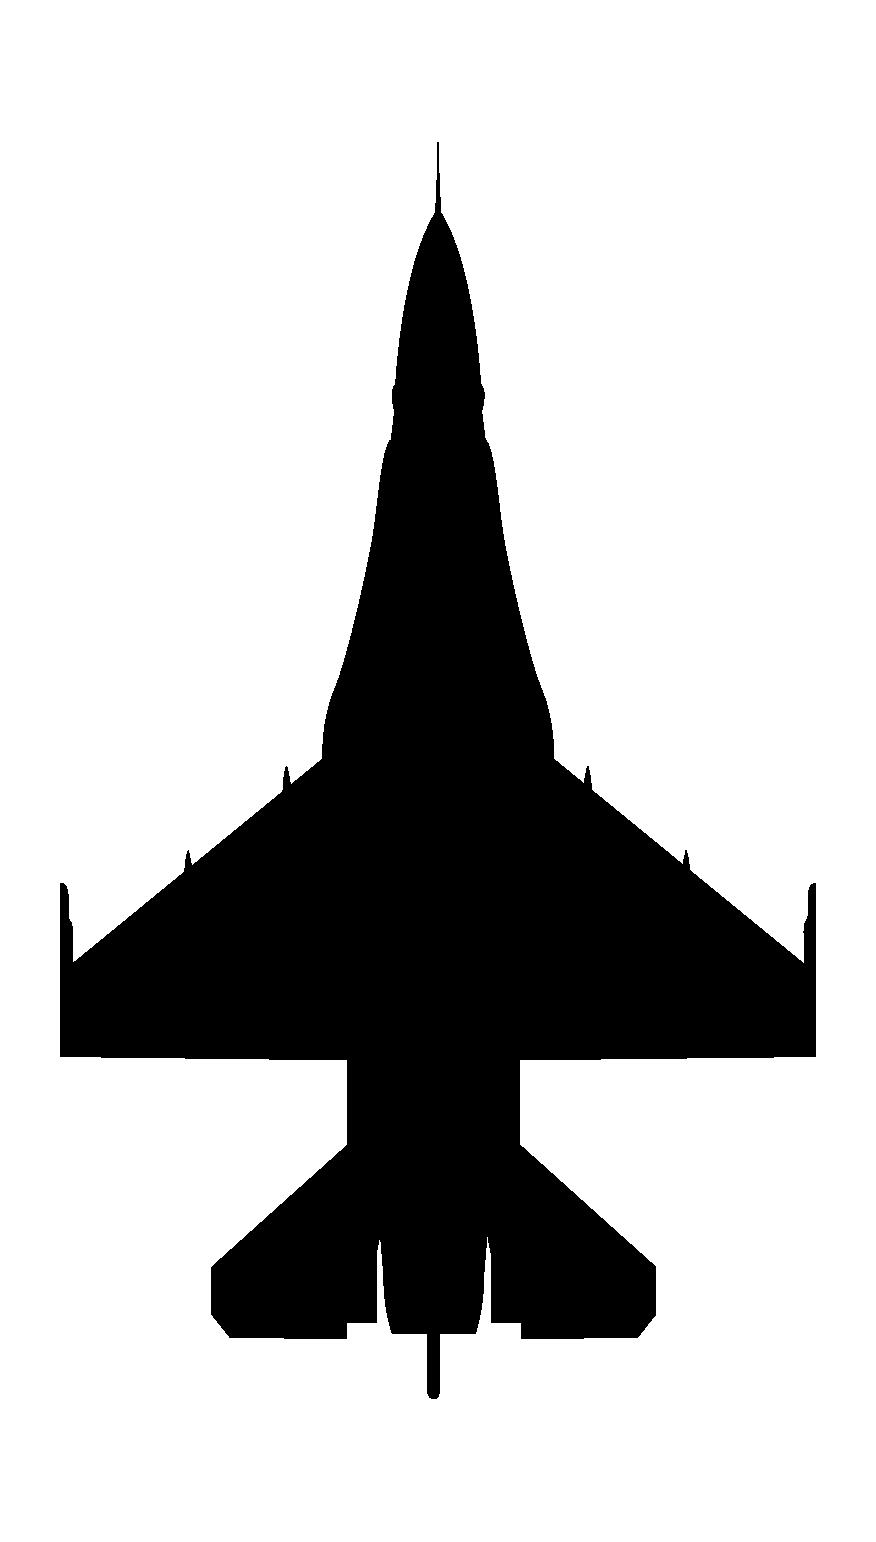
\includegraphics[
                    width=7.5mm,
                ]{diagrams/aircraft/silhouette_f16_top.pdf}
            };

            \node[anchor=north, font=\footnotesize] (1label) at (1fig.south) {1};
            \node[anchor=north, font=\footnotesize] (2label) at (2fig.south) {2};
            \node[anchor=north, font=\footnotesize] (3label) at (3fig.south) {3};
            \node[anchor=north, font=\footnotesize] (4label) at (4fig.south) {4};

        \end{tikzpicture}
        \caption{Finger four}
        \label{fig:supp_fig:form:fingerfour}
    \end{minipage}
\end{figure}

\begin{figure}[htbp]
    \centering
    \begin{minipage}[b]{0.5\textwidth}
        \centering
        \begin{tikzpicture}[figstyle]

            \coordinate (1) at (0,0);
            \coordinate (2) at ($(1)+(210:20)$);
            \coordinate (3) at ($(1)+(-30:20)$);
            \coordinate (4) at ($(3)+(-30:20)$);

            \draw[]
            (1) -- (2) 
            node[font=\footnotesize, above, pos=0.5, rotate=30] {0.1 nm}
            node[font=\footnotesize, below, pos=0.5, rotate=30] {30$^\circ$}
            (1) -- (3) 
            node[font=\footnotesize, above, pos=0.5, rotate=-30] {0.1 nm}
            node[font=\footnotesize, below, pos=0.5, rotate=-30] {30$^\circ$}
            (3) -- (4)
            node[font=\footnotesize, above, pos=0.5, rotate=-30] {0.1 nm}
            node[font=\footnotesize, below, pos=0.5, rotate=-30] {30$^\circ$};

            \node[yshift=-3mm] (1fig) at (1) {
                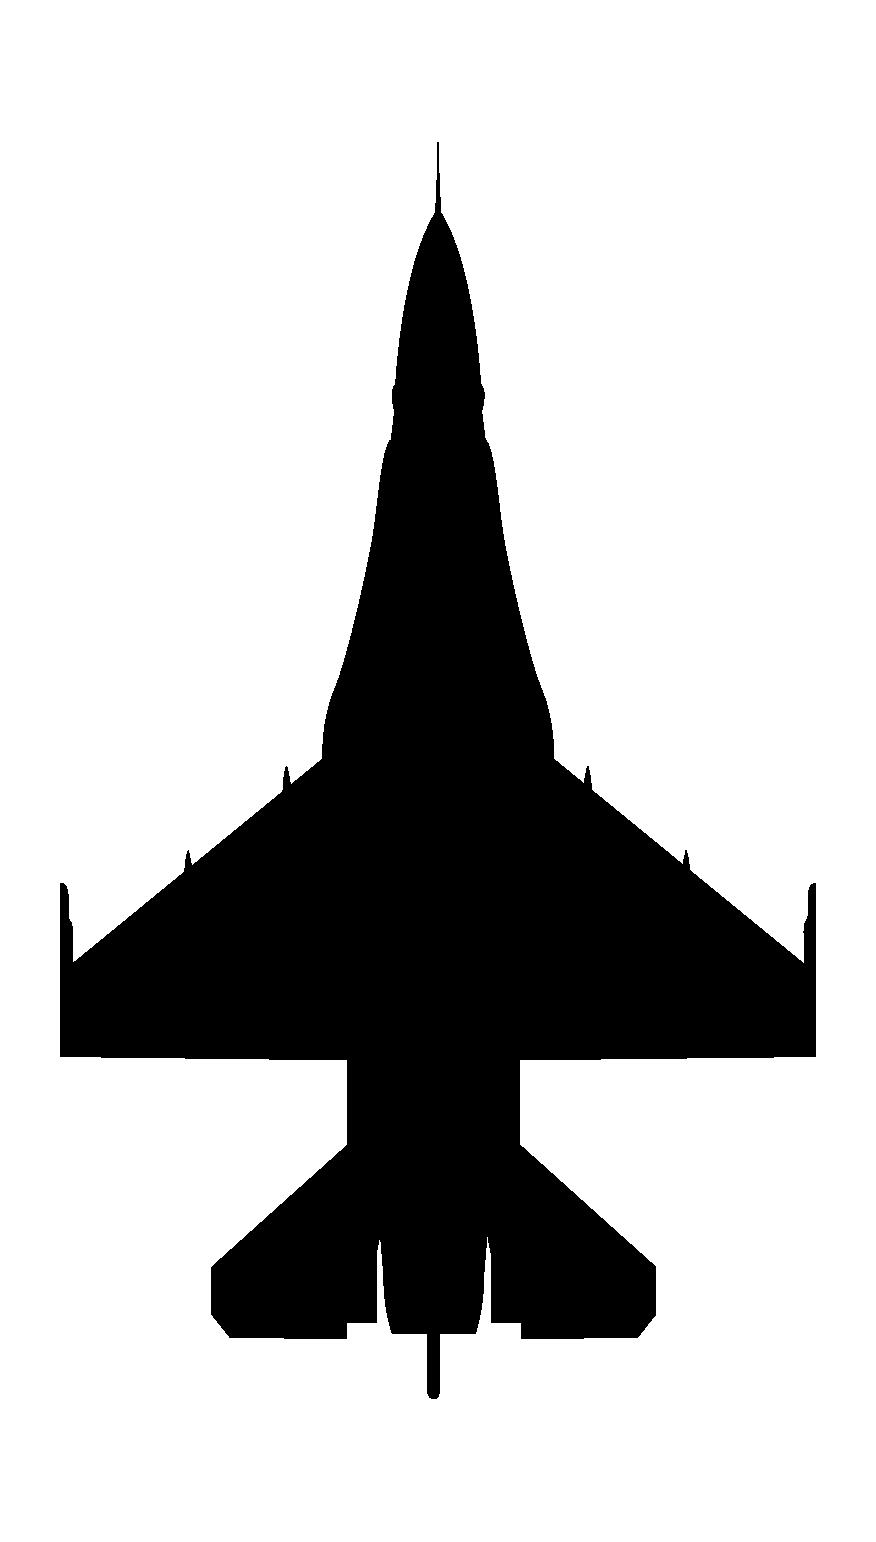
\includegraphics[
                    width=7.5mm,
                ]{diagrams/aircraft/silhouette_f16_top.pdf}
            };
            
            \node[yshift=-3mm] (2fig) at (2) {
                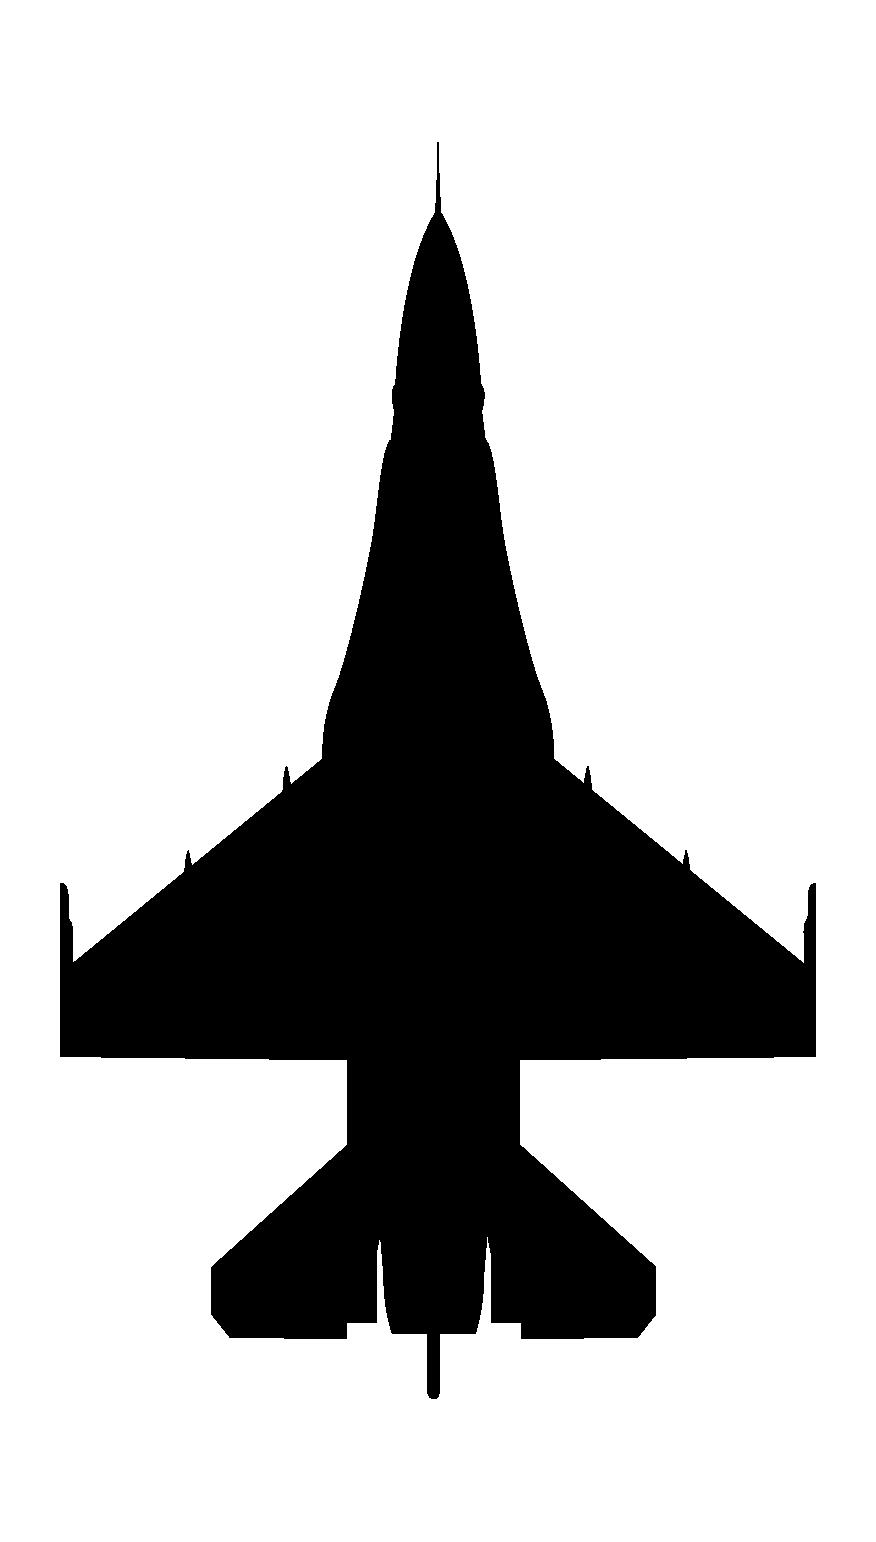
\includegraphics[
                    width=7.5mm,
                ]{diagrams/aircraft/silhouette_f16_top.pdf}
            };

            \node[yshift=-3mm] (3fig) at (3) {
                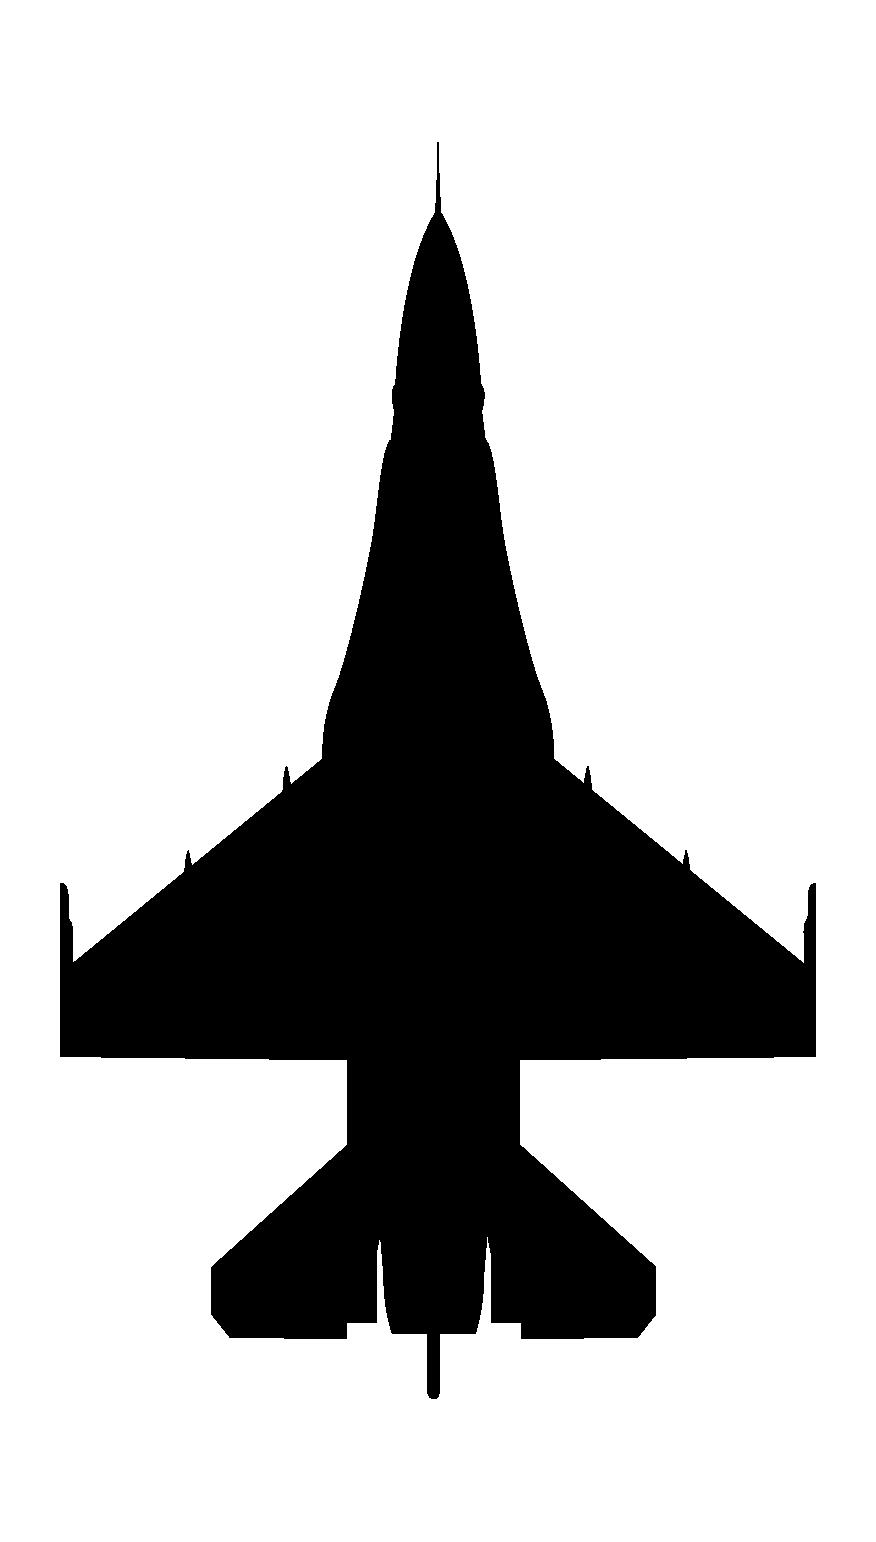
\includegraphics[
                    width=7.5mm,
                ]{diagrams/aircraft/silhouette_f16_top.pdf}
            };
            
            \node[yshift=-3mm] (4fig) at (4) {
                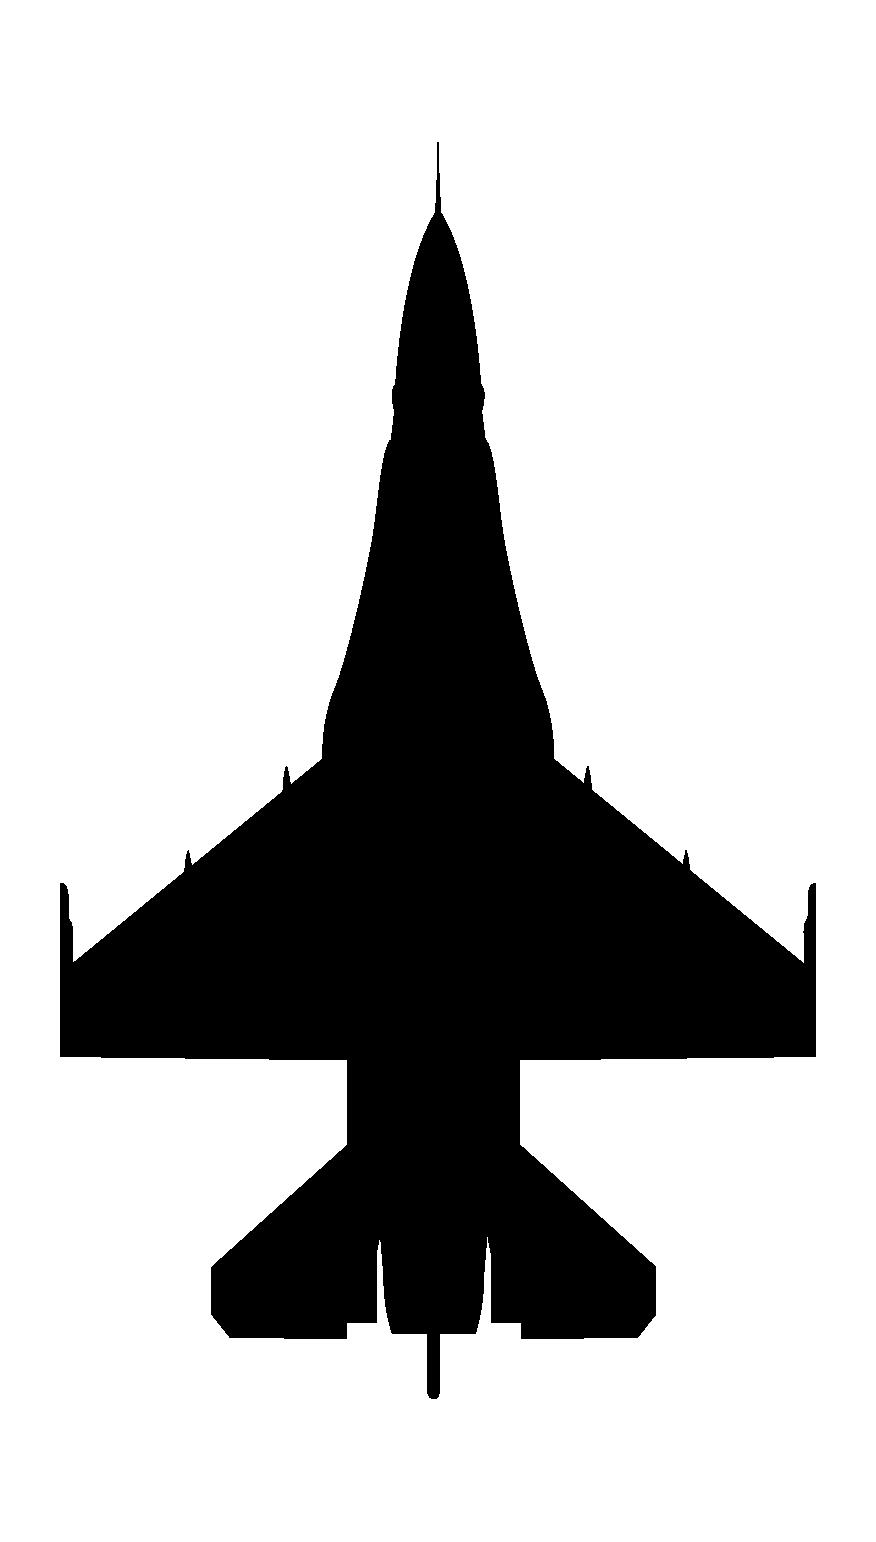
\includegraphics[
                    width=7.5mm,
                ]{diagrams/aircraft/silhouette_f16_top.pdf}
            };

            \node[anchor=north, font=\footnotesize] (1label) at (1fig.south) {1};
            \node[anchor=north, font=\footnotesize] (2label) at (2fig.south) {2};
            \node[anchor=north, font=\footnotesize] (3label) at (3fig.south) {3};
            \node[anchor=north, font=\footnotesize] (4label) at (4fig.south) {4};

        \end{tikzpicture}
        \caption{Route}
        \label{fig:supp_fig:form:route}
    \end{minipage}%
    \begin{minipage}[b]{0.5\textwidth}
        \centering
        \begin{tikzpicture}[figstyle]
            
            \coordinate (1) at (0,0);
            \coordinate (2) at ($(1)+(-45:10)$);
            \coordinate (3) at ($(2)+(-45:10)$);
            \coordinate (4) at ($(3)+(-45:10)$);

            \node[yshift=-2mm] (1fig) at (1) {
                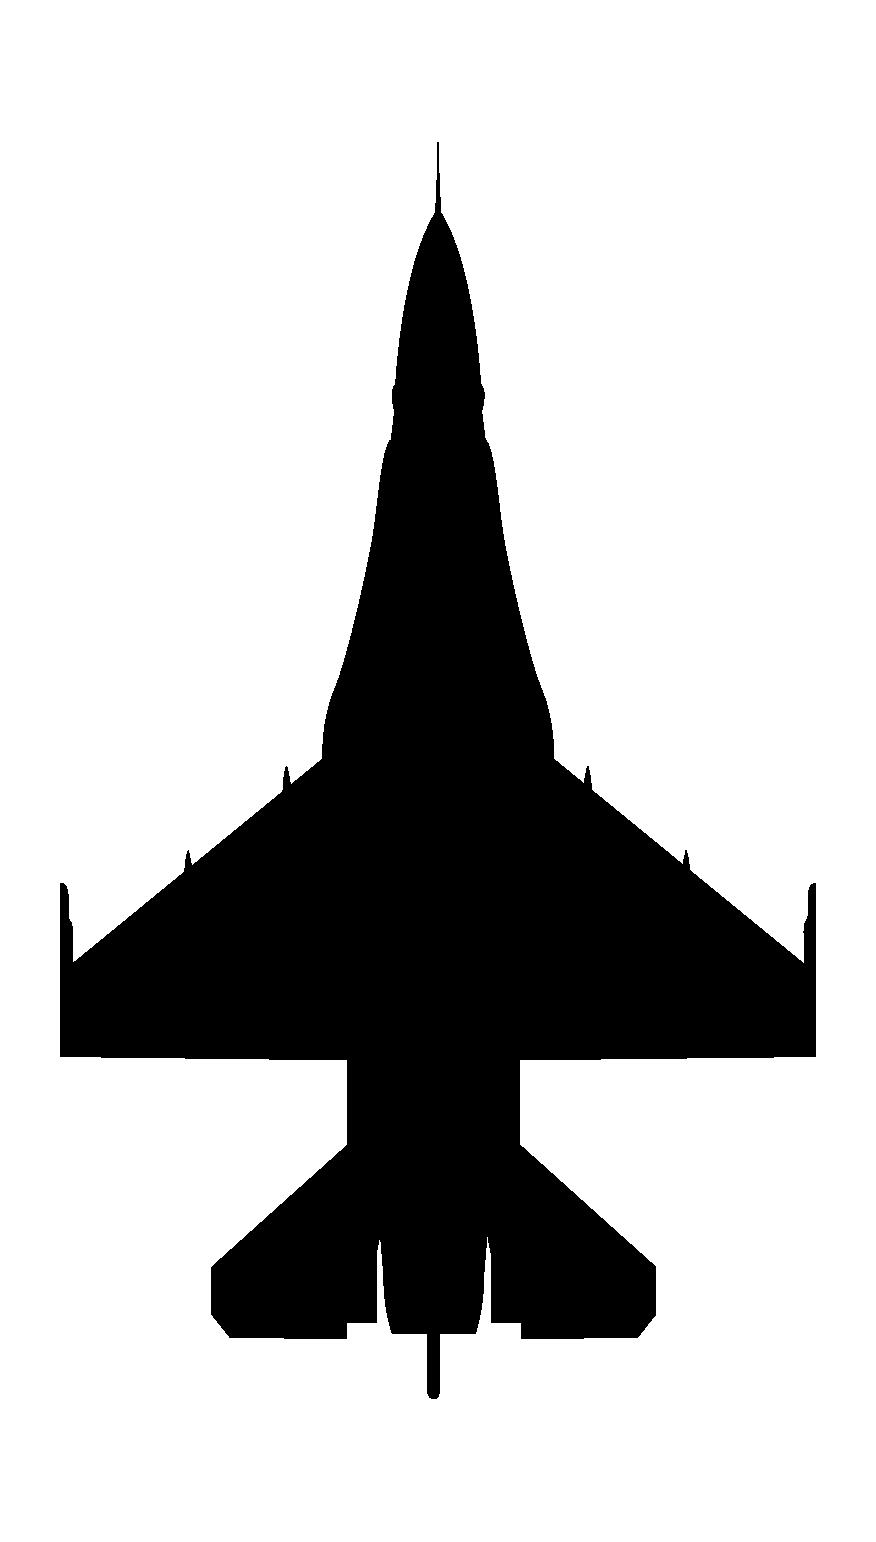
\includegraphics[
                    width=7.5mm,
                ]{diagrams/aircraft/silhouette_f16_top.pdf}
            };
            
            \node[yshift=-2mm] (2fig) at (2) {
                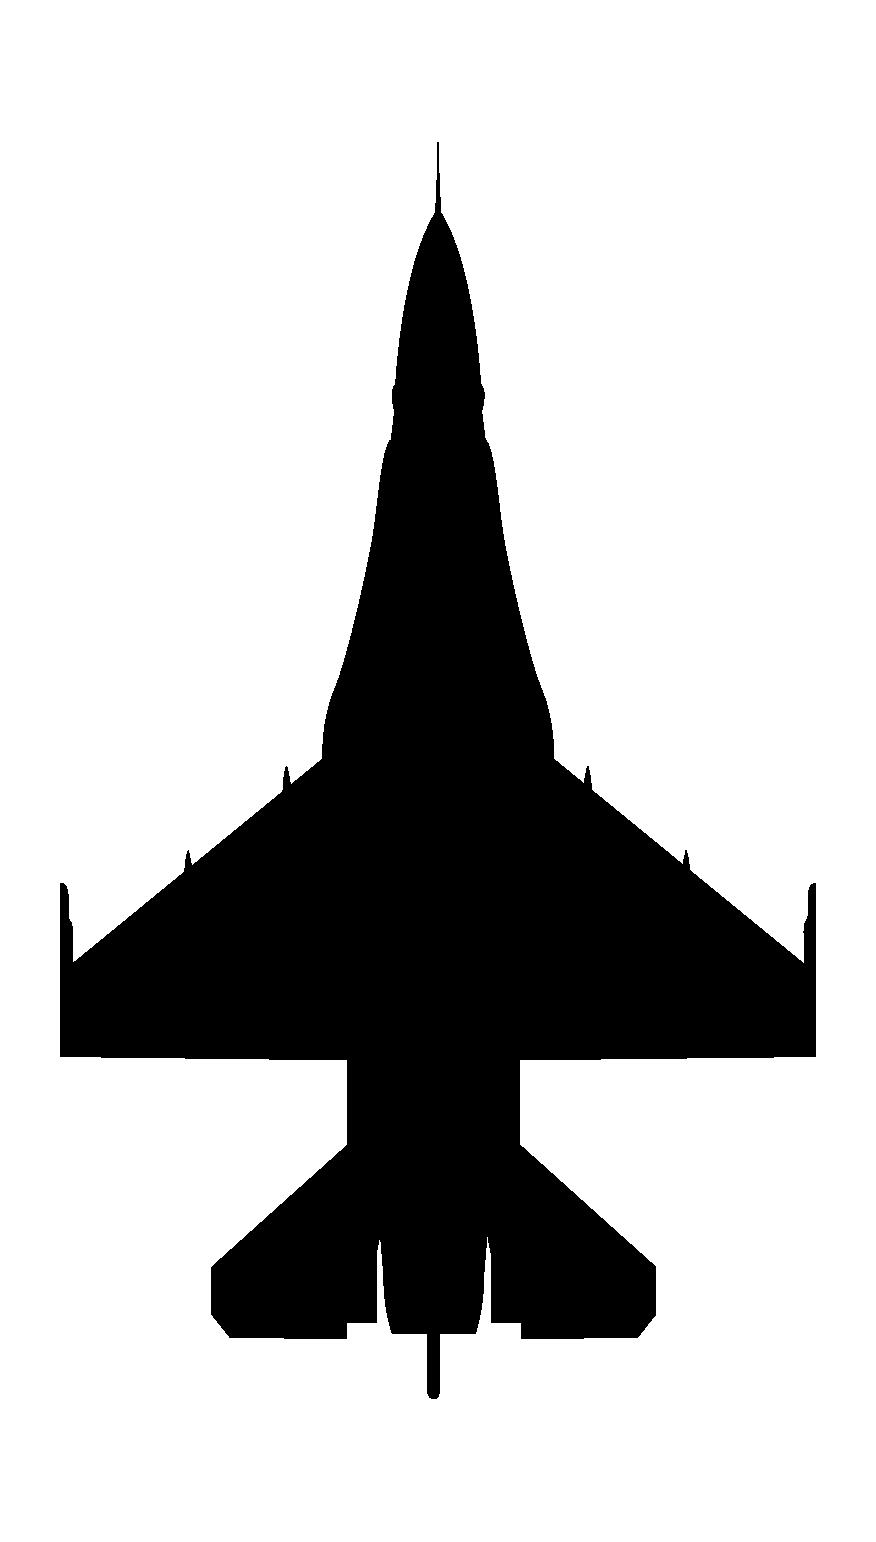
\includegraphics[
                    width=7.5mm,
                ]{diagrams/aircraft/silhouette_f16_top.pdf}
            };

            \node[yshift=-2mm] (3fig) at (3) {
                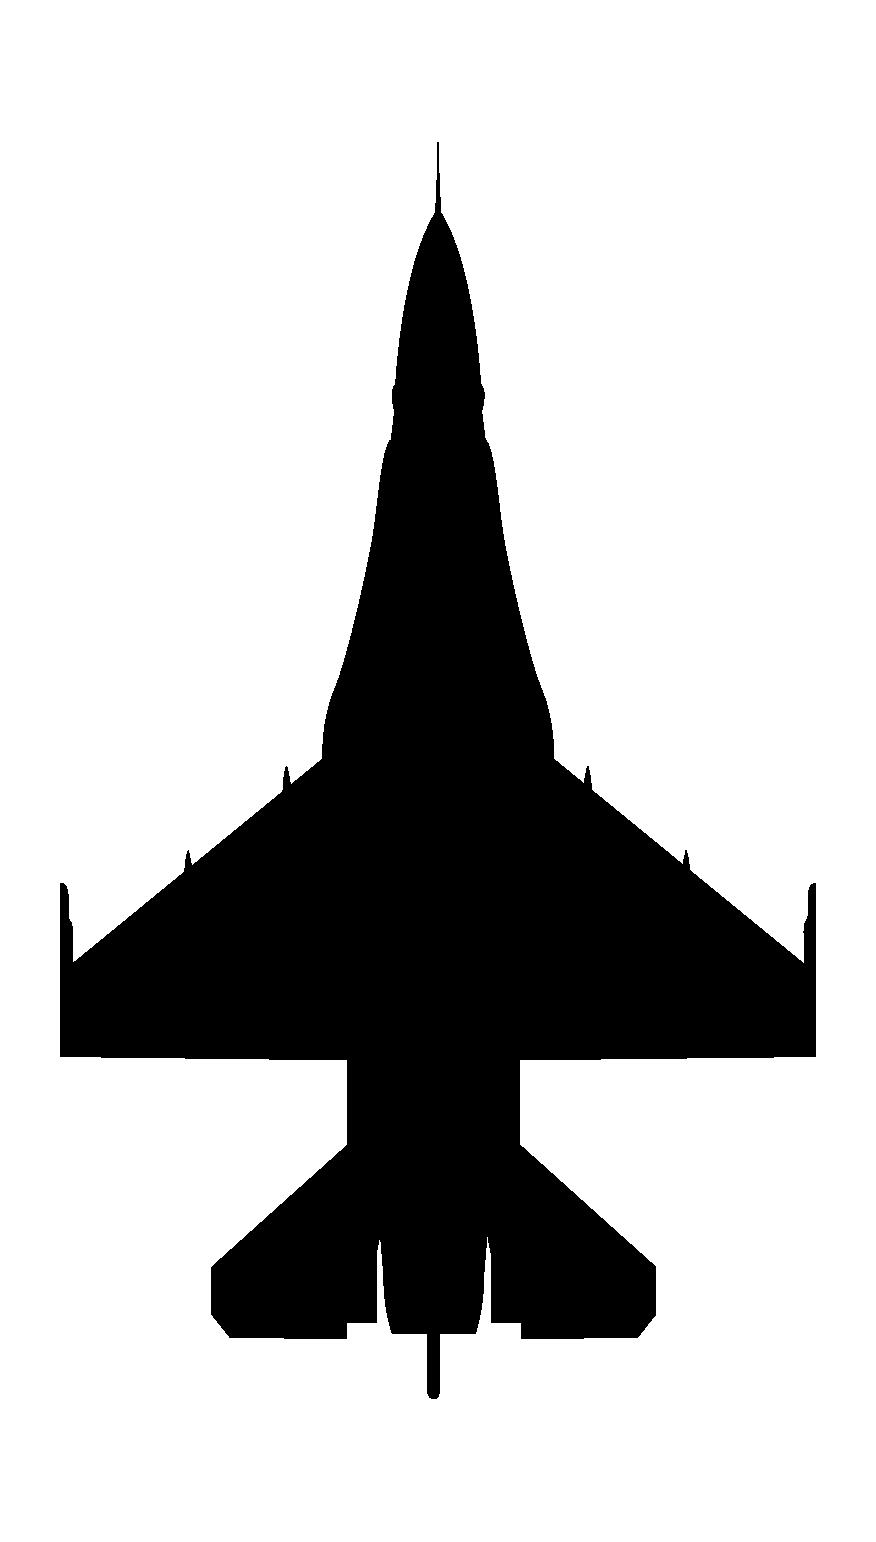
\includegraphics[
                    width=7.5mm,
                ]{diagrams/aircraft/silhouette_f16_top.pdf}
            };
            
            \node[yshift=-2mm] (4fig) at (4) {
                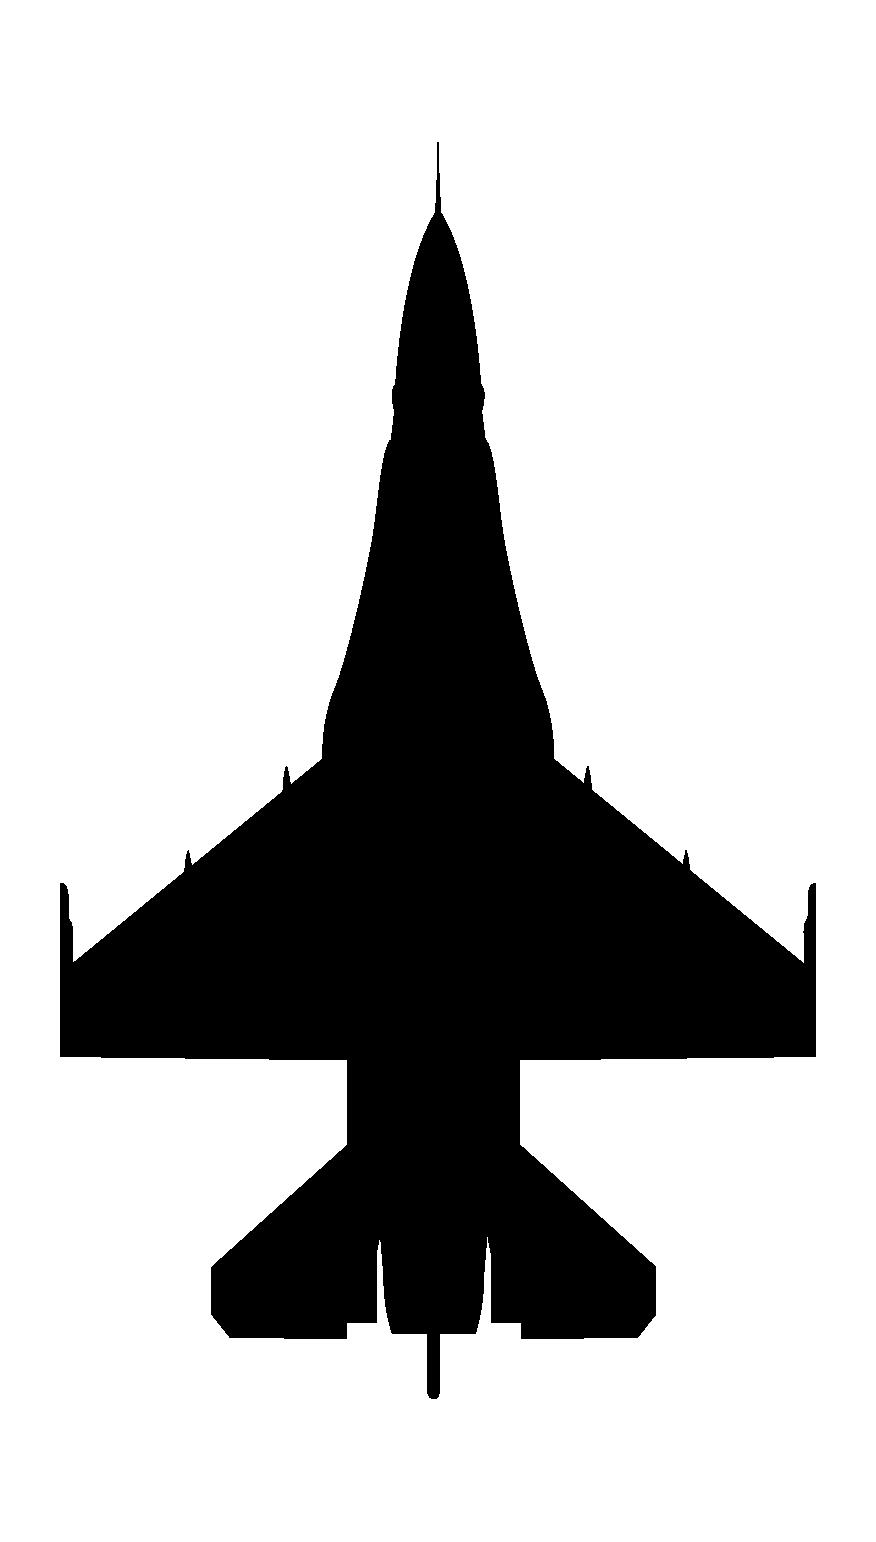
\includegraphics[
                    width=7.5mm,
                ]{diagrams/aircraft/silhouette_f16_top.pdf}
            };

            \node[anchor=north, font=\footnotesize] (1label) at (1fig.south) {1};
            \node[anchor=north, font=\footnotesize] (2label) at (2fig.south) {2};
            \node[anchor=north, font=\footnotesize] (3label) at (3fig.south) {3};
            \node[anchor=north, font=\footnotesize] (4label) at (4fig.south) {4};

        \end{tikzpicture}
        \caption{Echelon right}
        \label{fig:supp_fig:form:echelonright}
    \end{minipage}
\end{figure}

\paragraph{Line Abreast} 
\textbf{Tactical formation}
--- allows simultaneous weapons employment,
mutual cover

\medskip
\textbf{Disadvantages} --- requires continuous monitoring to maintain

\hfill\textbf{Reference \cref{fig:supp_fig:form:4shiplab}}

\paragraph{Spread} 
\textbf{Relaxed line abreast} 
--- more room for wingman to maneuver, easier to maintain

\hfill\textbf{Reference \cref{fig:supp_fig:form:4shipspread}}

\paragraph{Fluid Four}
\textbf{Relaxed line abreast} --- wingmen in fighting wing

\hfill\textbf{Reference \cref{fig:supp_fig:form:fluidfour}}

\begin{figure}[htbp]
    \centering
    \begin{tikzpicture}[figstyle]
            
        \coordinate (1) at (0,0);
        \coordinate (2) at ($(1)+(180:20)$);
        \coordinate (3) at ($(1)+(0:20)$);
        \coordinate (4) at ($(3)+(0:20)$);
        
        \draw[]
        (1) -- (2)
        node[font=\footnotesize, above, pos=0.5] {LAB}
        (1) -- (3)
        node[font=\footnotesize, above, pos=0.5] {LAB}
        (3) -- (4)
        node[font=\footnotesize, above, pos=0.5] {LAB};

        \node[yshift=-2mm] (1fig) at (1) {
            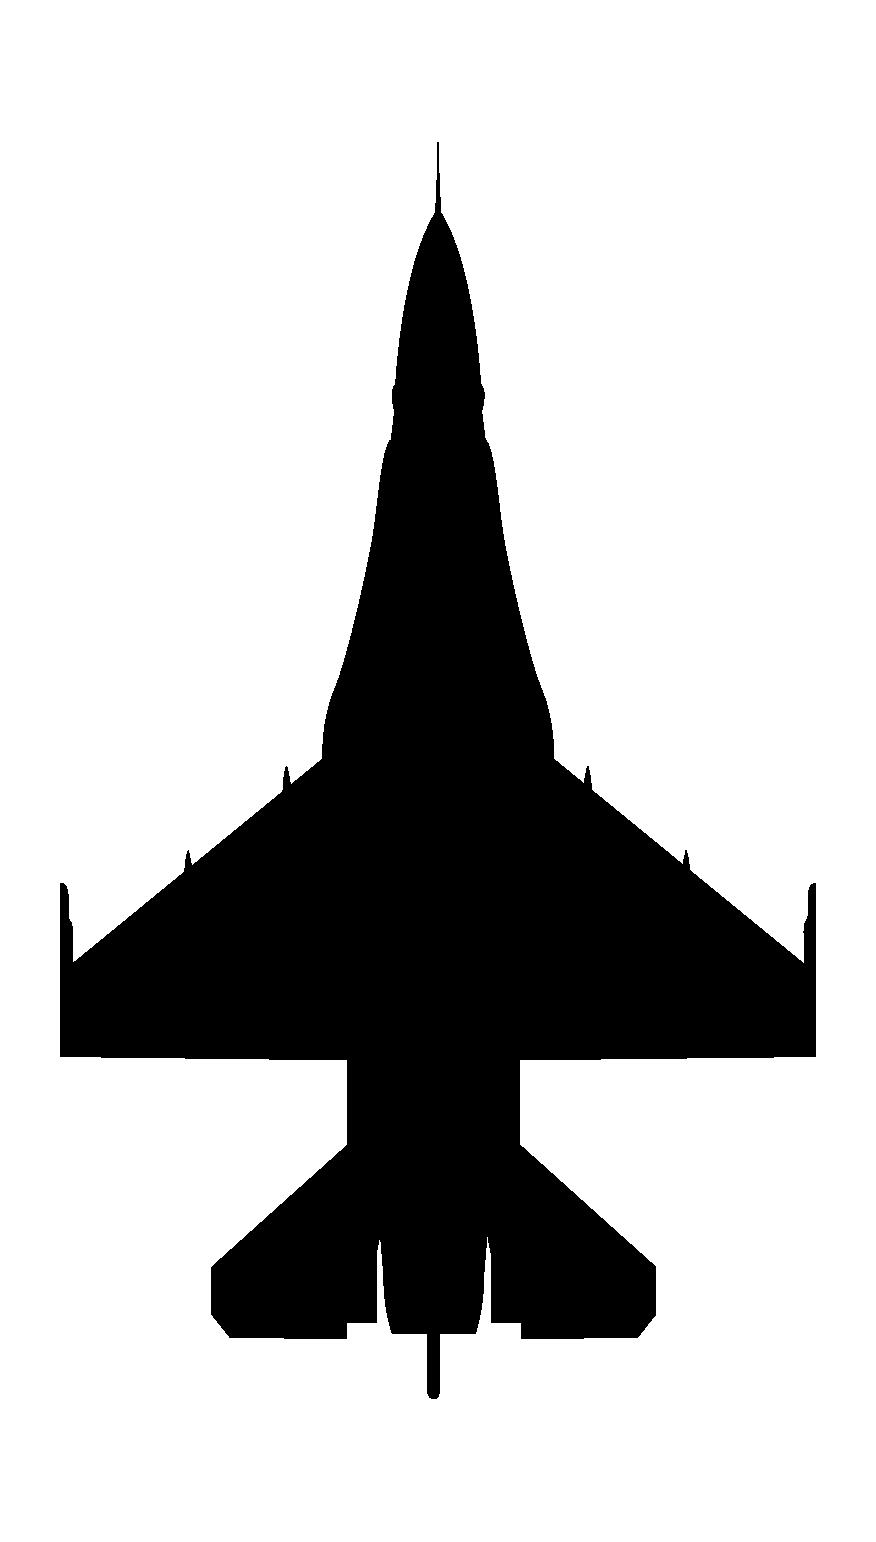
\includegraphics[
                width=7.5mm,
            ]{diagrams/aircraft/silhouette_f16_top.pdf}
        };
        
        \node[yshift=-2mm] (2fig) at (2) {
            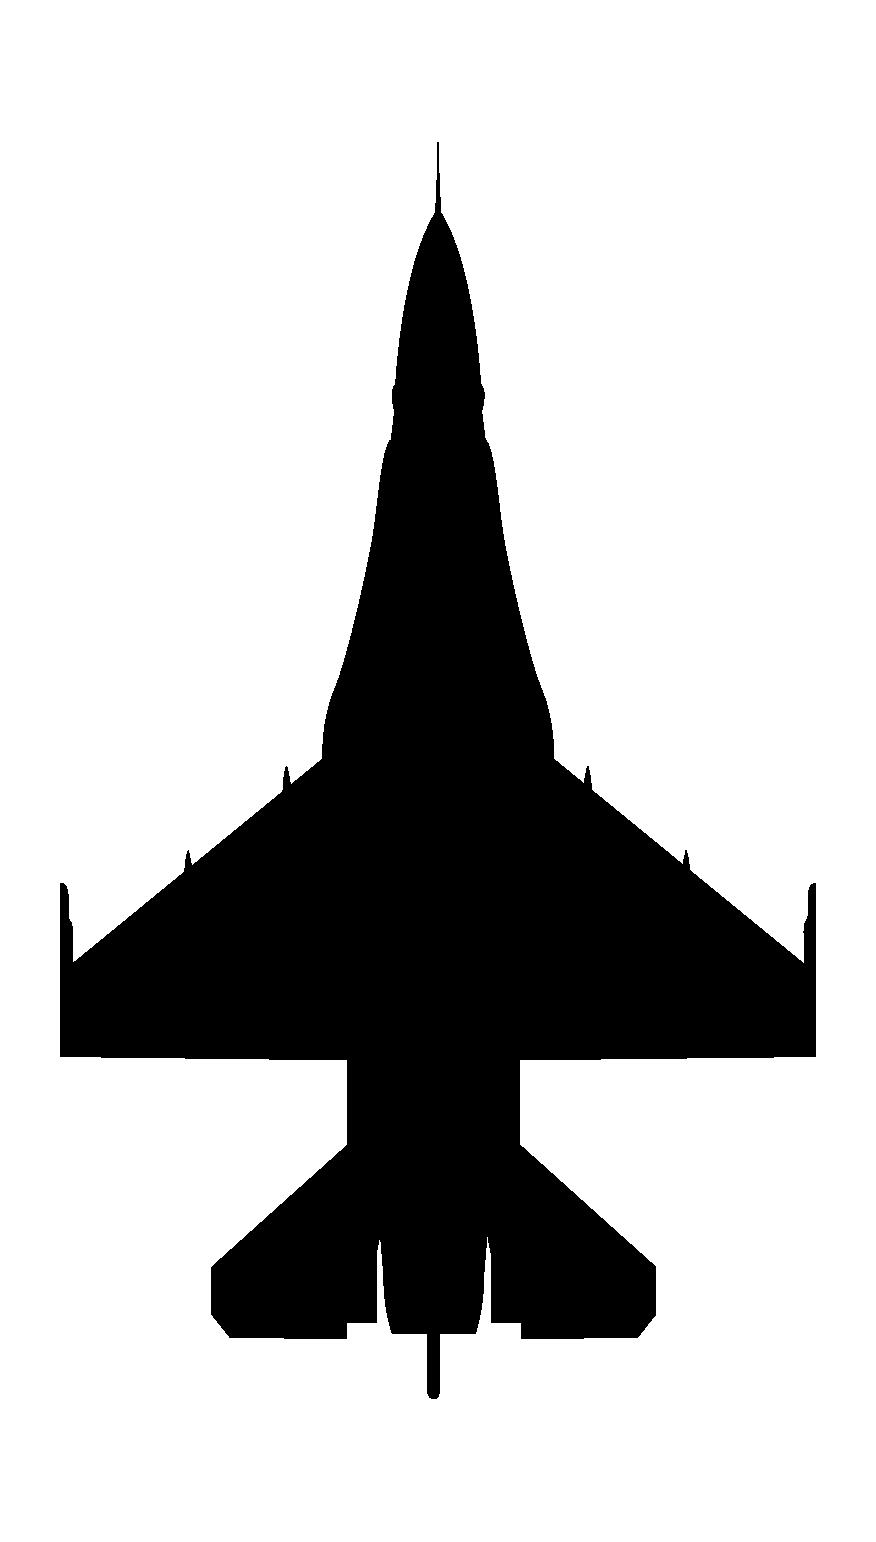
\includegraphics[
                width=7.5mm,
            ]{diagrams/aircraft/silhouette_f16_top.pdf}
        };

        \node[yshift=-2mm] (3fig) at (3) {
            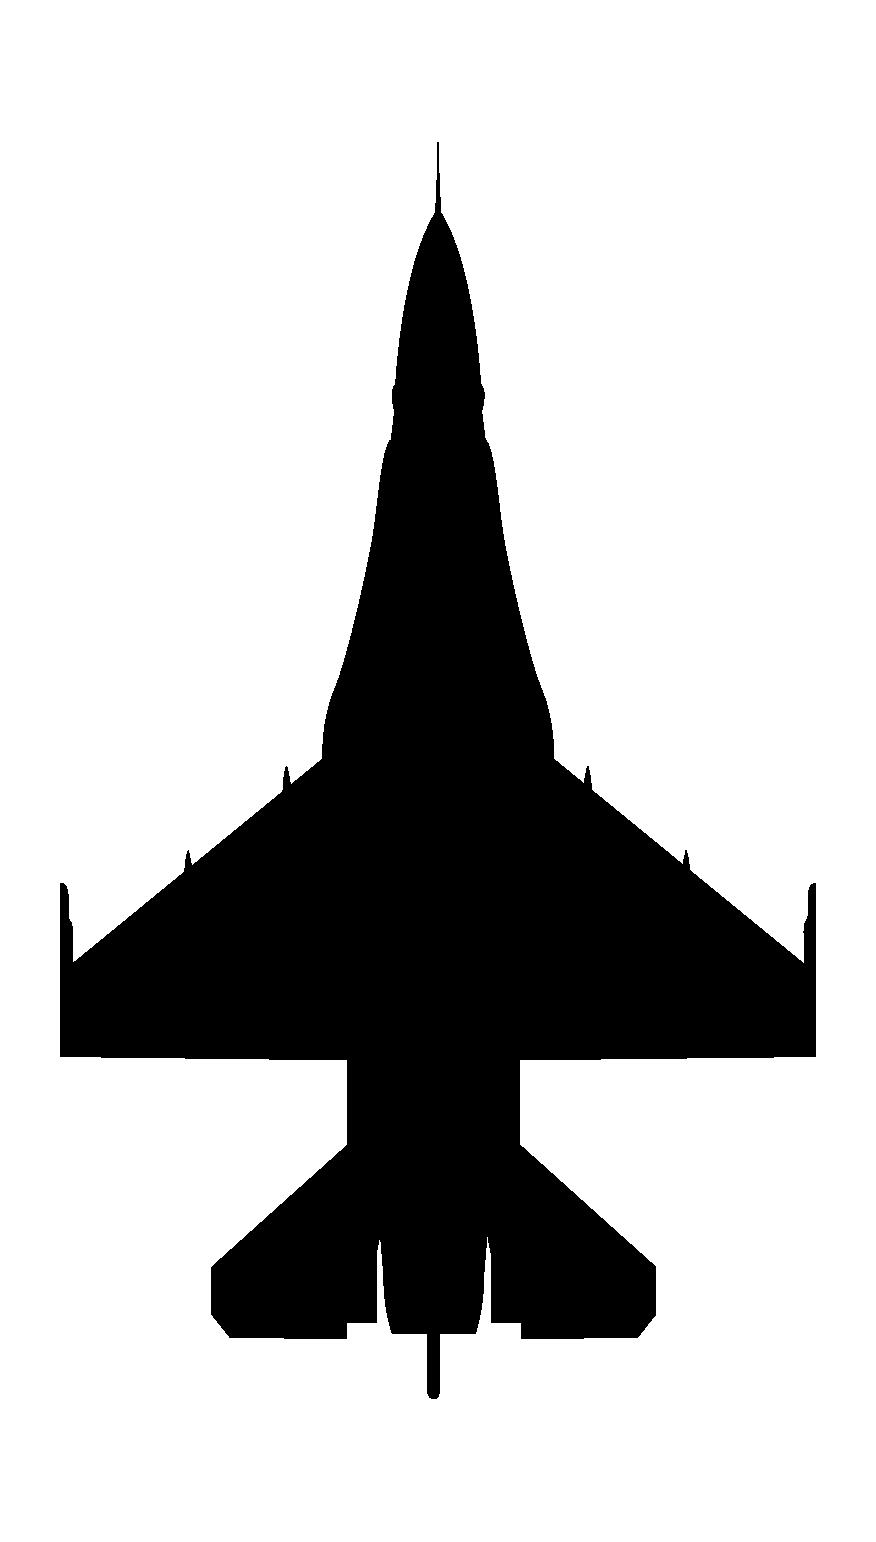
\includegraphics[
                width=7.5mm,
            ]{diagrams/aircraft/silhouette_f16_top.pdf}
        };
        
        \node[yshift=-2mm] (4fig) at (4) {
            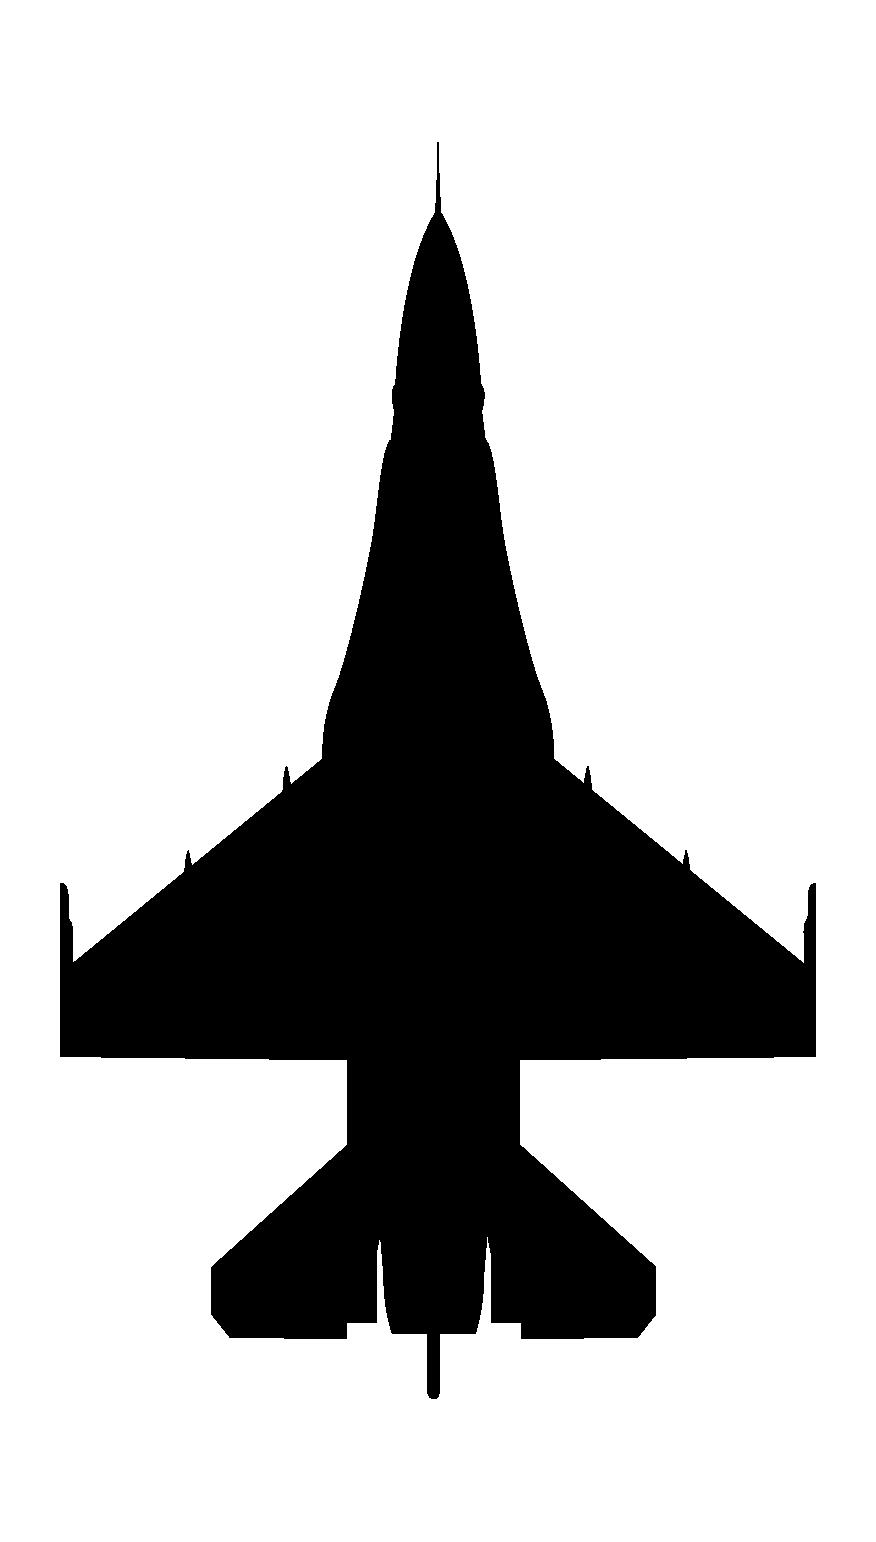
\includegraphics[
                width=7.5mm,
            ]{diagrams/aircraft/silhouette_f16_top.pdf}
        };

        \node[anchor=north, font=\footnotesize] (1label) at (1fig.south) {1};
        \node[anchor=north, font=\footnotesize] (2label) at (2fig.south) {2};
        \node[anchor=north, font=\footnotesize] (3label) at (3fig.south) {3};
        \node[anchor=north, font=\footnotesize] (4label) at (4fig.south) {4};

    \end{tikzpicture}
    \caption{Four-ship line abreast (LAB)}
    \label{fig:supp_fig:form:4shiplab}
\end{figure}

\begin{figure}[htbp]
    \centering
    \begin{tikzpicture}[figstyle]
    
        \coordinate (1) at (0,0);
        \coordinate (2) at ($(1)+(190:20)$);
        \coordinate (3) at ($(1)+(0:20)$);
        \coordinate (4) at ($(3)+(-10:20)$);

        % \draw[dashed]
        % (lead) -- ++(0:20) arc (0:-20:20) -- (lead);

        \draw[fill=color2!15]
        ($(1)+(180:10)$) 
        -- ++(180:20) 
        node[font=\footnotesize, above, pos=0.5] {0.6-1.0 nm}
        node[font=\footnotesize, left, pos=1] {0$^\circ$}
        arc (180:210:30)
        node[font=\footnotesize, left, pos=1] {30$^\circ$}
        -- ($(1)+(210:10)$) 
        arc (210:180:10);
        \draw[]
        (1) -- (3)
        node[font=\footnotesize, above, pos=0.5] {LAB};
        \draw[fill=color2!15]
        ($(3)+(0:10)$) 
        -- ++(0:20) node[font=\footnotesize, above, pos=0.5] {0.6-1.0 nm}
        node[font=\footnotesize, right, pos=1] {0$^\circ$}
        arc (0:-30:30)
        node[font=\footnotesize, right, pos=1] {30$^\circ$}
        -- ($(3)+(-30:10)$) 
        arc (-30:0:10);

        \node[yshift=-3mm] (1fig) at (1) {
            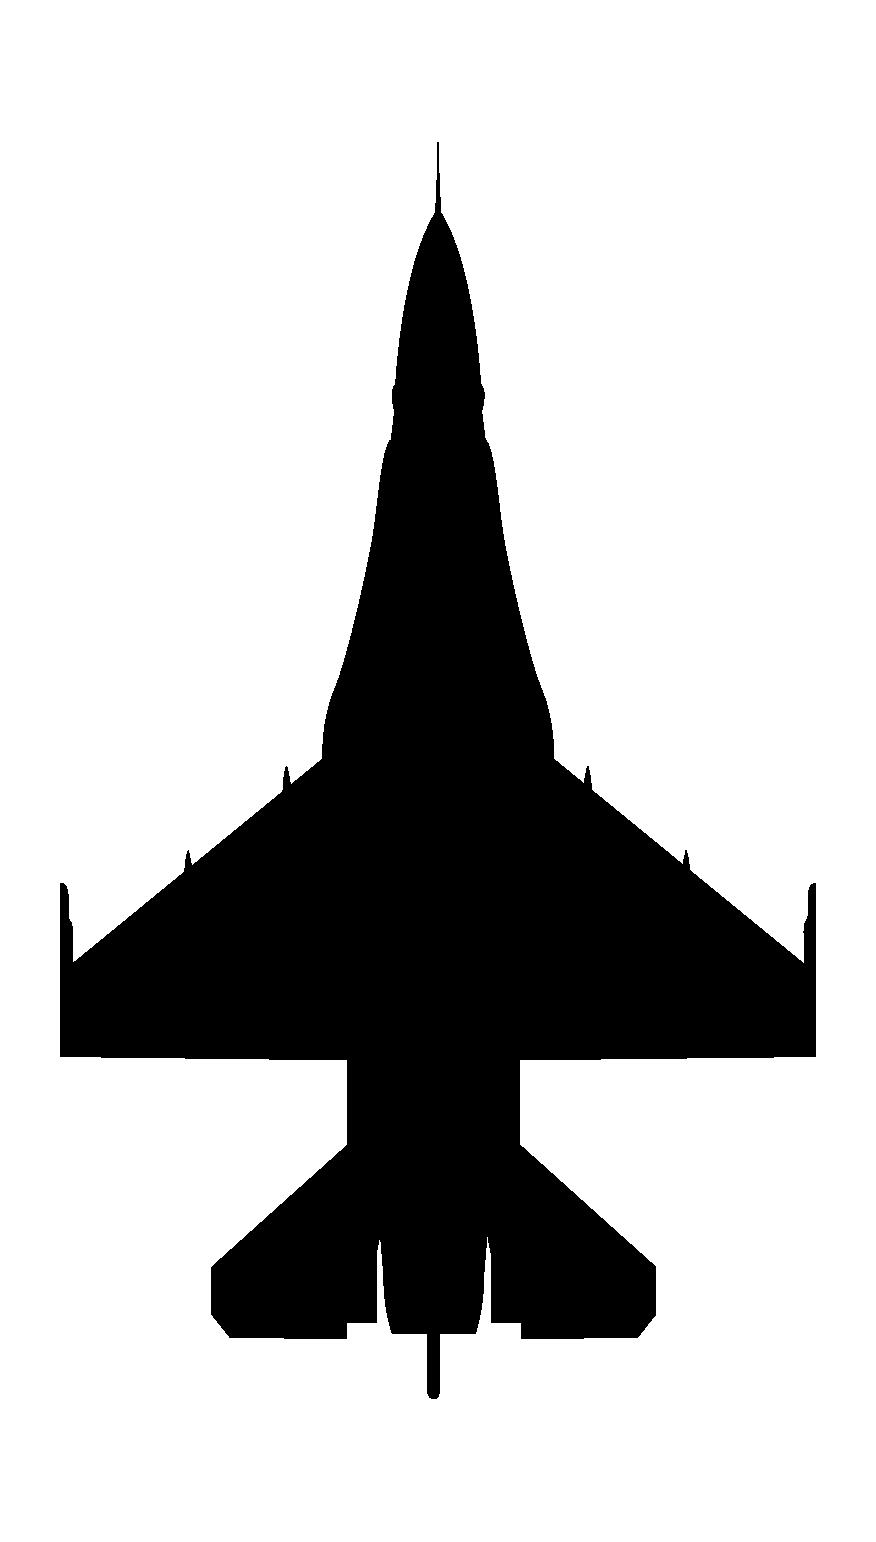
\includegraphics[
                width=7.5mm,
            ]{diagrams/aircraft/silhouette_f16_top.pdf}
        };
        
        \node[yshift=-3mm] (2fig) at (2) {
            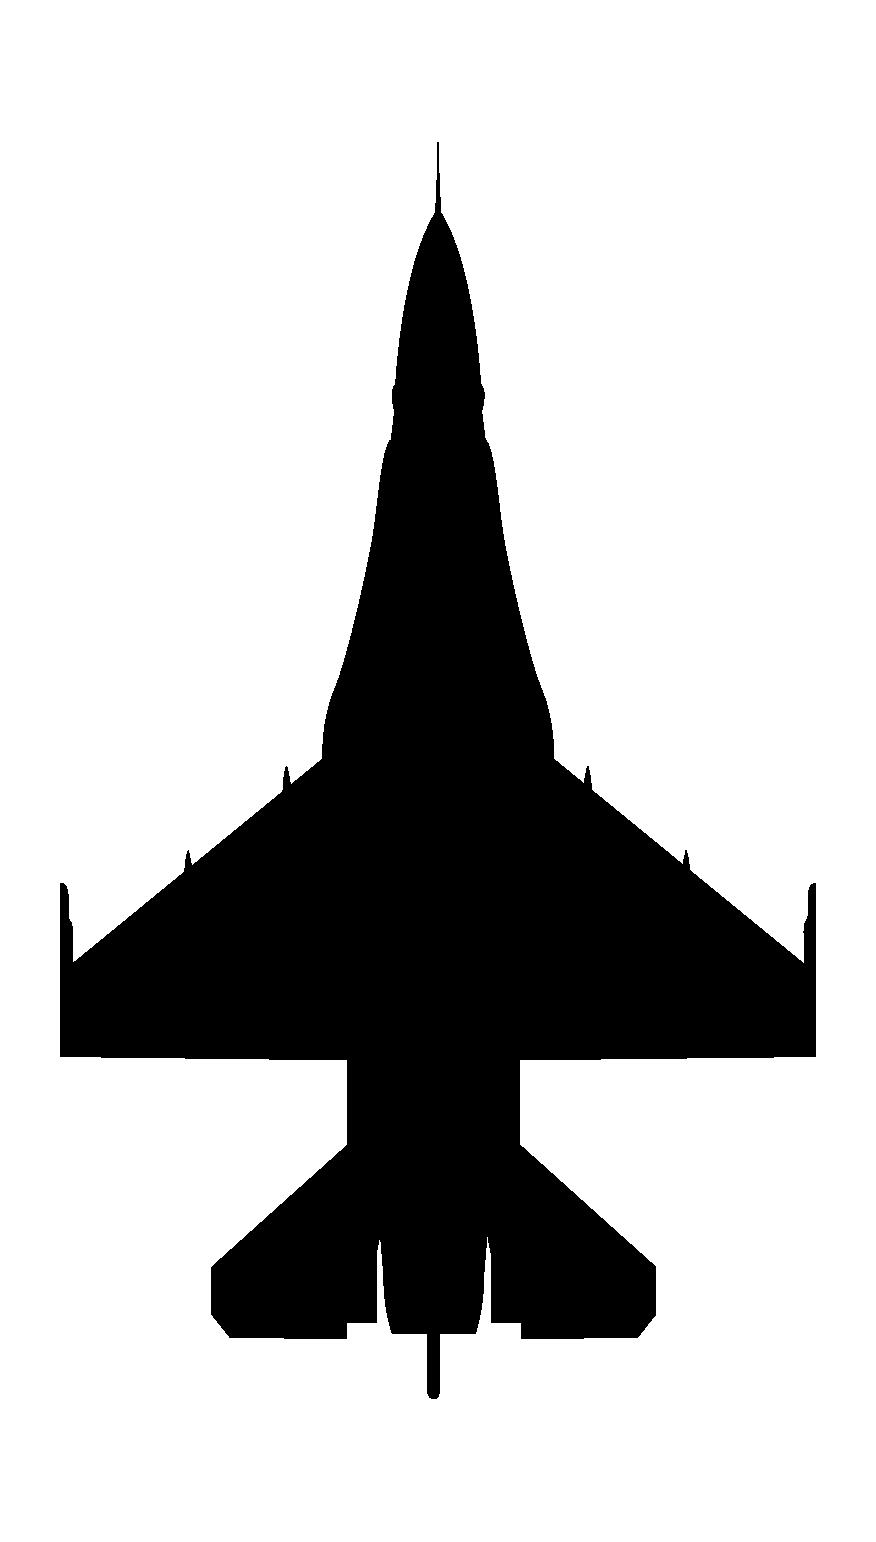
\includegraphics[
                width=7.5mm,
            ]{diagrams/aircraft/silhouette_f16_top.pdf}
        };

        \node[yshift=-3mm] (3fig) at (3) {
            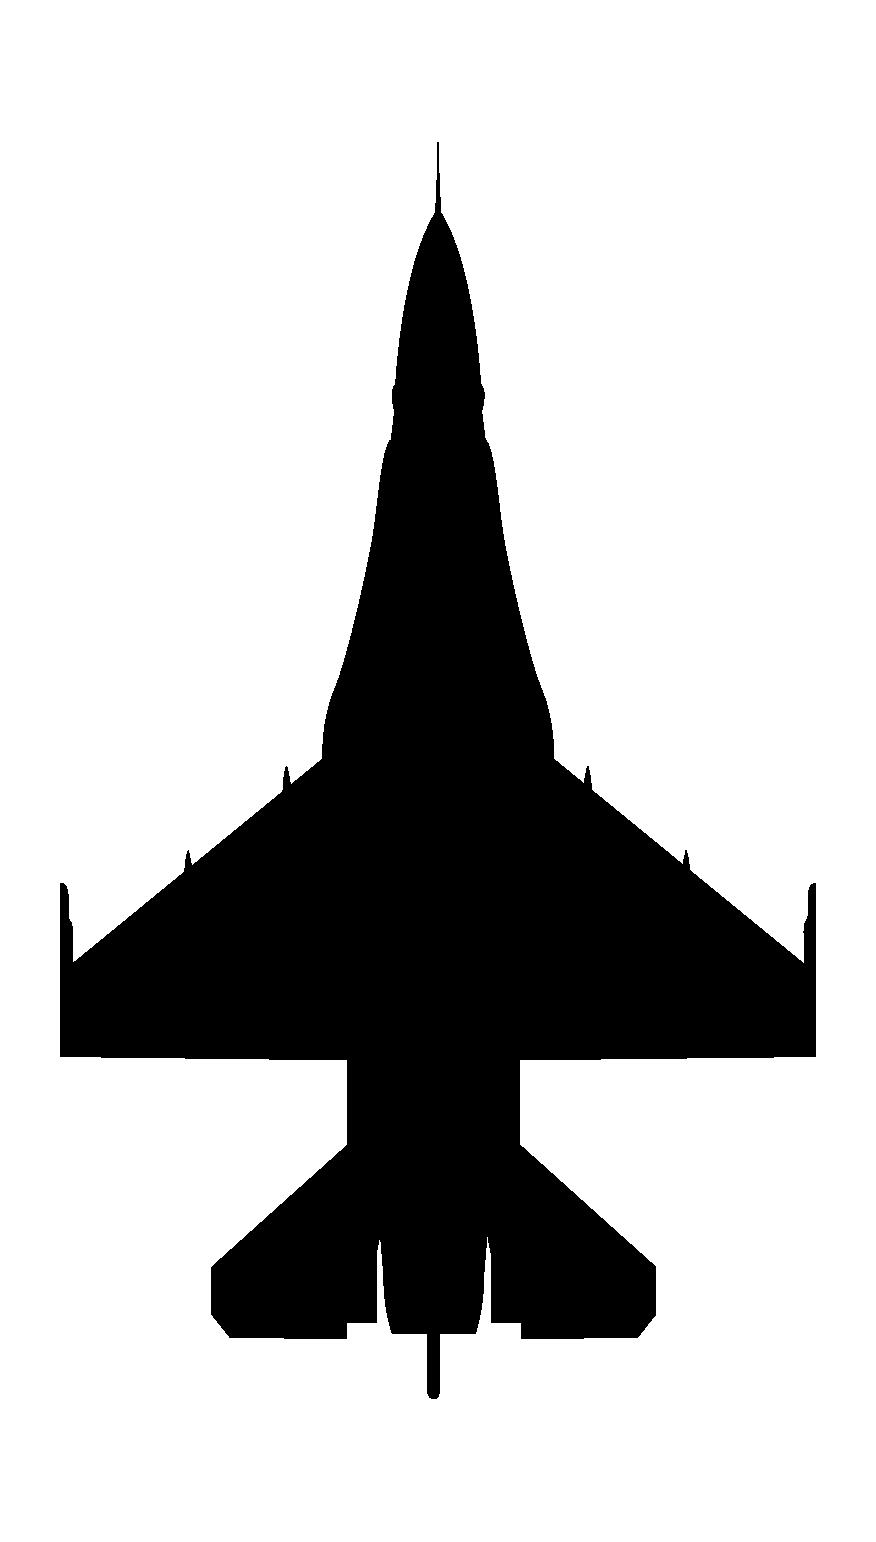
\includegraphics[
                width=7.5mm,
            ]{diagrams/aircraft/silhouette_f16_top.pdf}
        };
        
        \node[yshift=-3mm] (4fig) at (4) {
            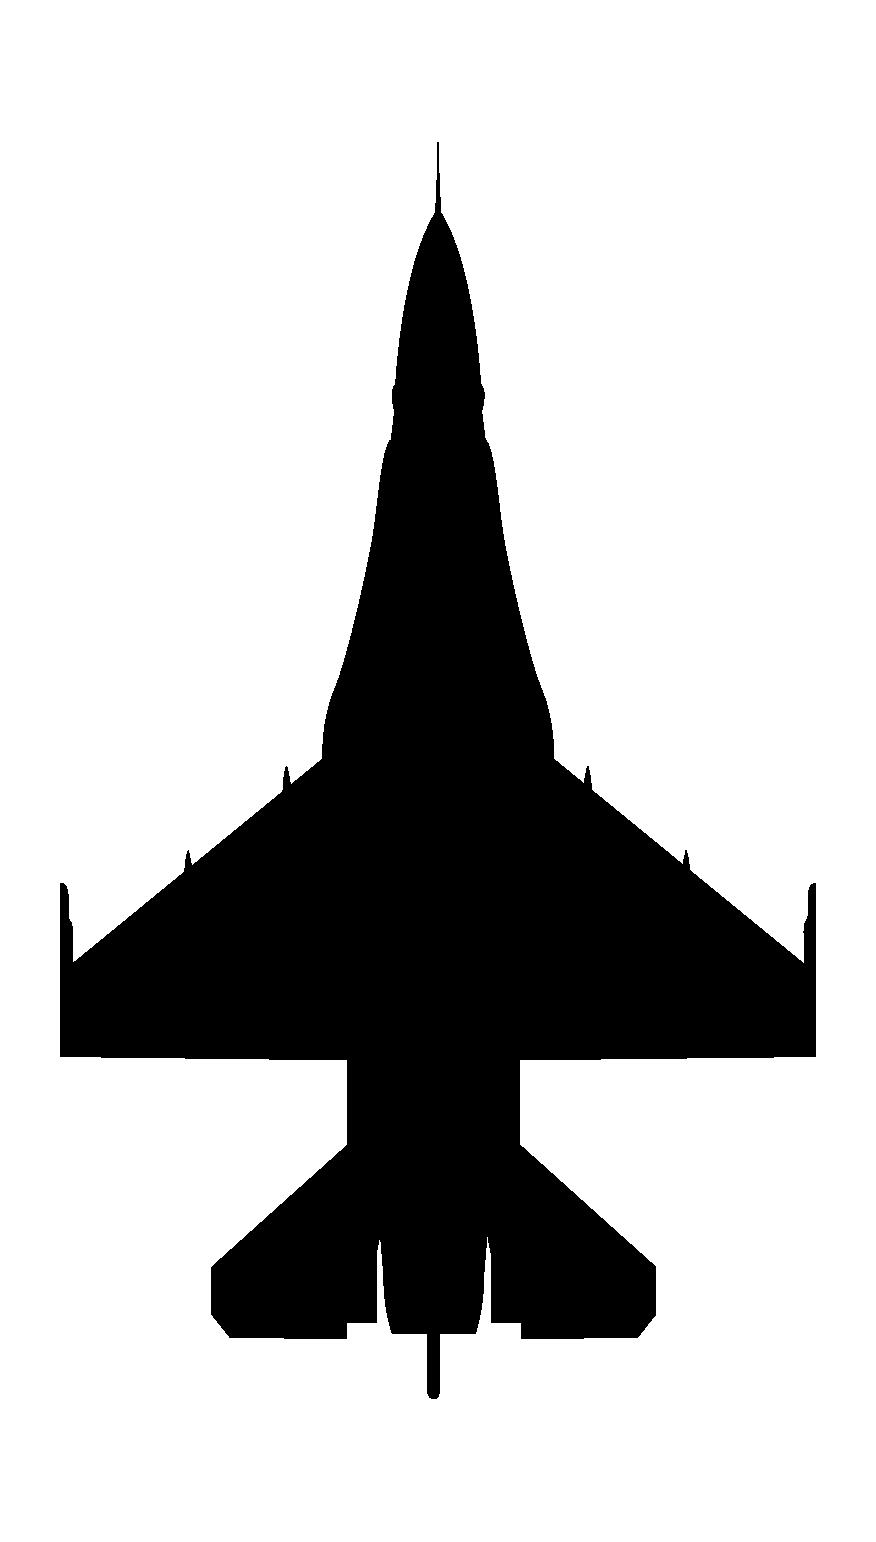
\includegraphics[
                width=7.5mm,
            ]{diagrams/aircraft/silhouette_f16_top.pdf}
        };

        \node[anchor=north, font=\footnotesize] (1label) at (1fig.south) {1};
        \node[anchor=north, font=\footnotesize] (2label) at (2fig.south) {2};
        \node[anchor=north, font=\footnotesize] (3label) at (3fig.south) {3};
        \node[anchor=north, font=\footnotesize] (4label) at (4fig.south) {4};

    \end{tikzpicture}
    \caption{Four-ship spread}
    \label{fig:supp_fig:form:4shipspread}
\end{figure}

\begin{figure}[htbp]
    \centering
    \begin{tikzpicture}[figstyle]
    
        \coordinate (1) at (0,0);
        \coordinate (2) at ($(1)+(220:20)$);
        \coordinate (3) at ($(1)+(0:20)$);
        \coordinate (4) at ($(3)+(-40:20)$);

        % \draw[dashed]
        % (lead) -- ++(0:20) arc (0:-20:20) -- (lead);

        \draw[fill=color2!15]
        ($(1)+(210:10)$) 
        -- ++(210:20) 
        node[font=\footnotesize, above left, pos=0.5] {Fighting Wing}
        node[font=\footnotesize, left, pos=1] {30$^\circ$}
        arc (210:240:30)
        node[font=\footnotesize, below, pos=1] {60$^\circ$}
        -- ($(1)+(240:10)$) 
        node[font=\footnotesize, right, pos=0.25] {2}
        arc (240:210:10);
        \draw[]
        (1) -- (3)
        node[font=\footnotesize, above, pos=0.5] {LAB};
        \draw[fill=color2!15]
        ($(3)+(-30:10)$) 
        -- ++(-30:20) 
        node[font=\footnotesize, above right, pos=0.5] {Fighting Wing}
        node[font=\footnotesize, right, pos=1] {30$^\circ$}
        arc (-30:-60:30)
        node[font=\footnotesize, below, pos=1] {60$^\circ$}
        -- ($(3)+(-60:10)$) 
        node[font=\footnotesize, left, pos=0.25] {4}
        arc (-60:-30:10);

        \node[yshift=-3mm] (1fig) at (1) {
            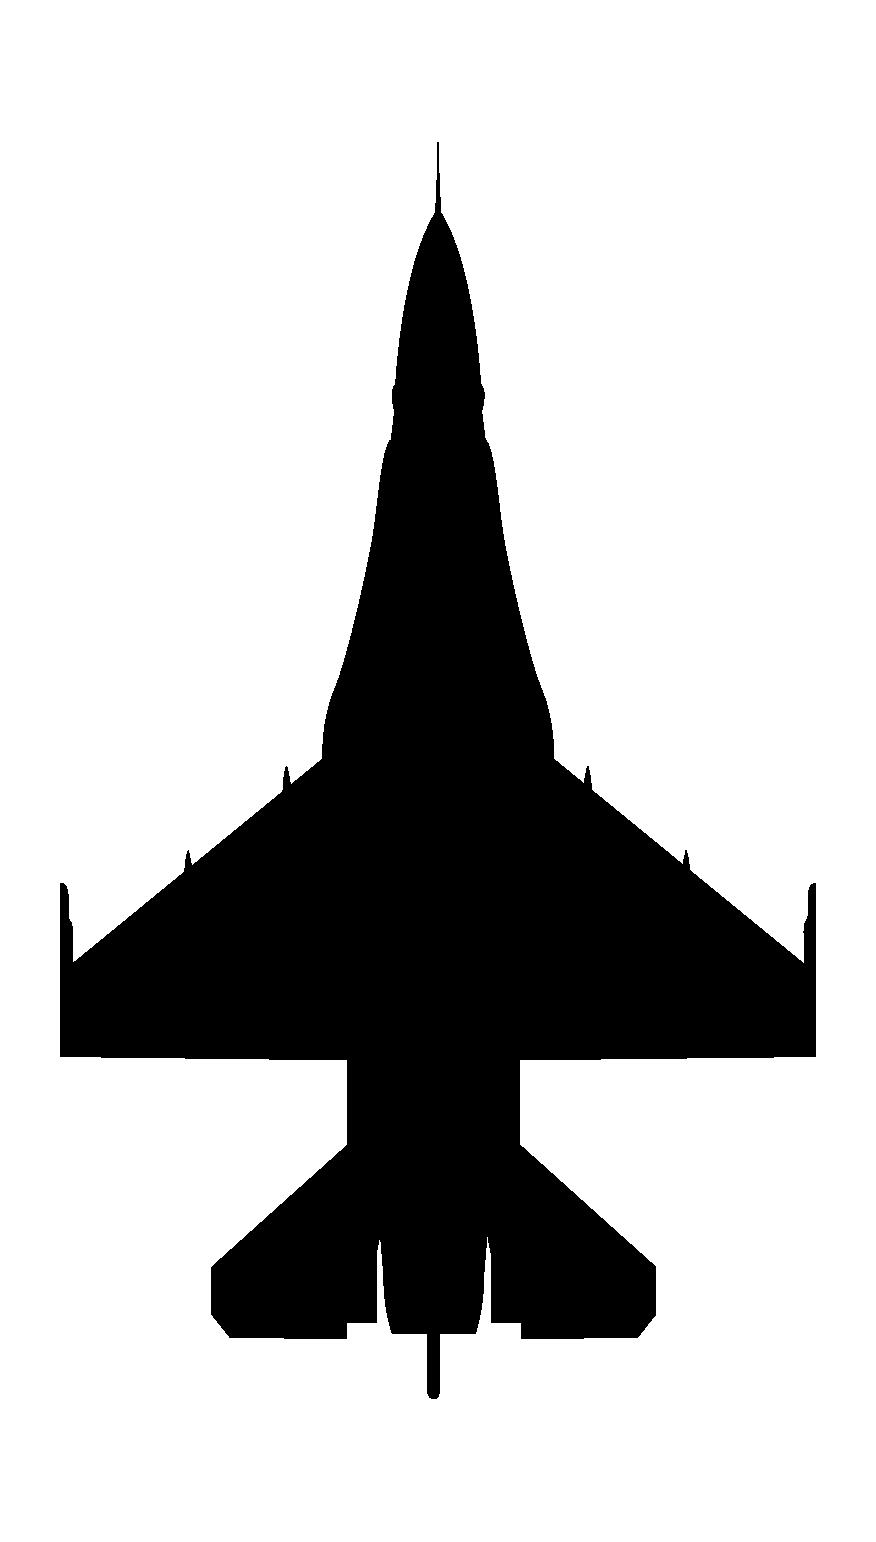
\includegraphics[
                width=7.5mm,
            ]{diagrams/aircraft/silhouette_f16_top.pdf}
        };
        
        \node[yshift=-3mm] (2fig) at (2) {
            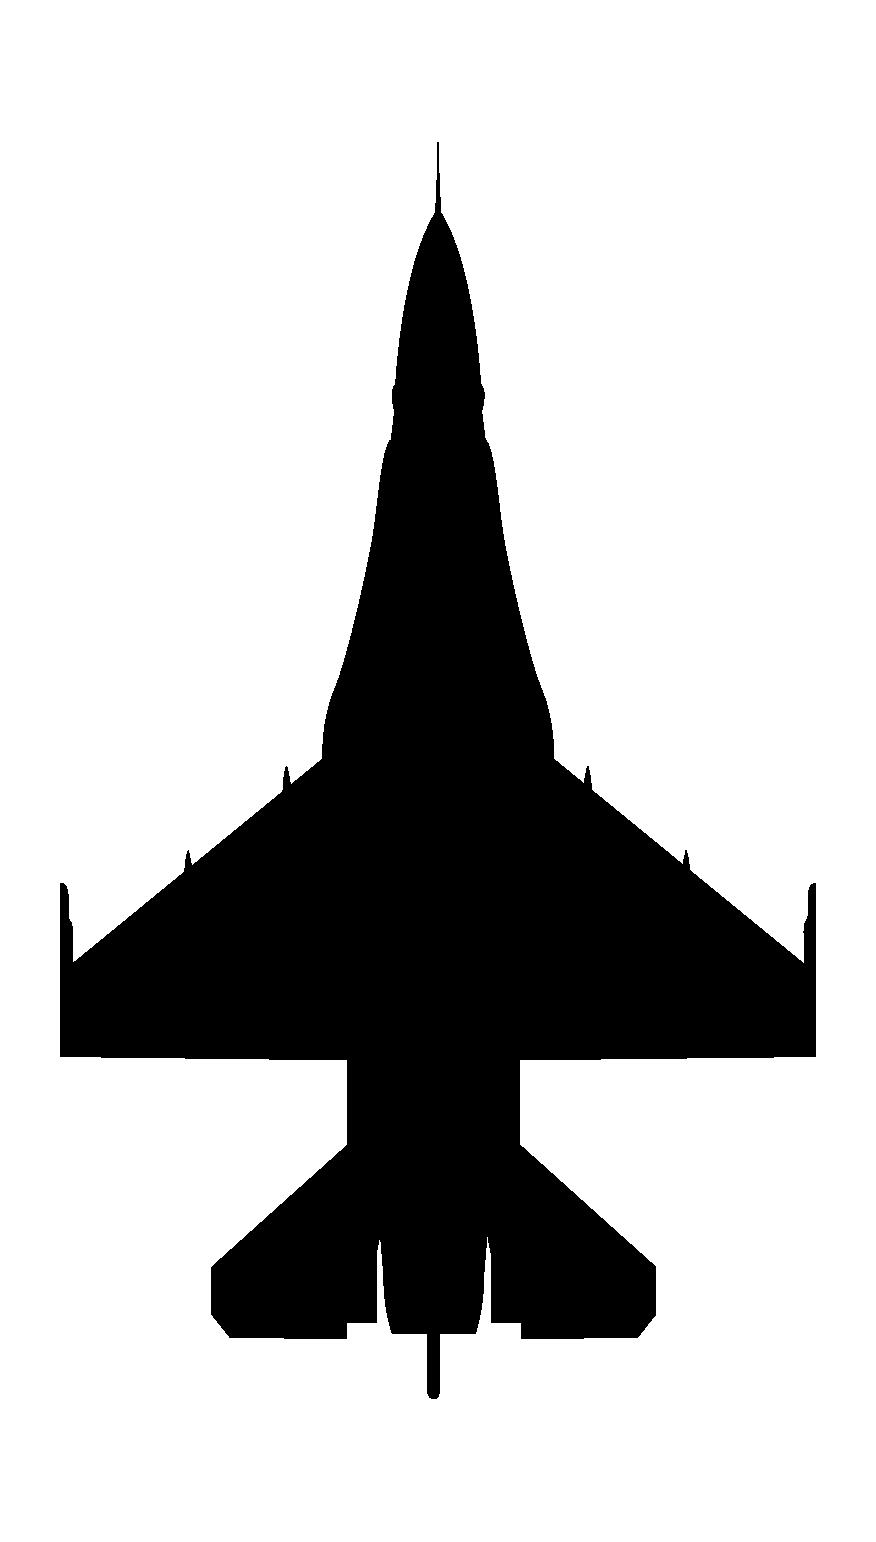
\includegraphics[
                width=7.5mm,
            ]{diagrams/aircraft/silhouette_f16_top.pdf}
        };

        \node[yshift=-3mm] (3fig) at (3) {
            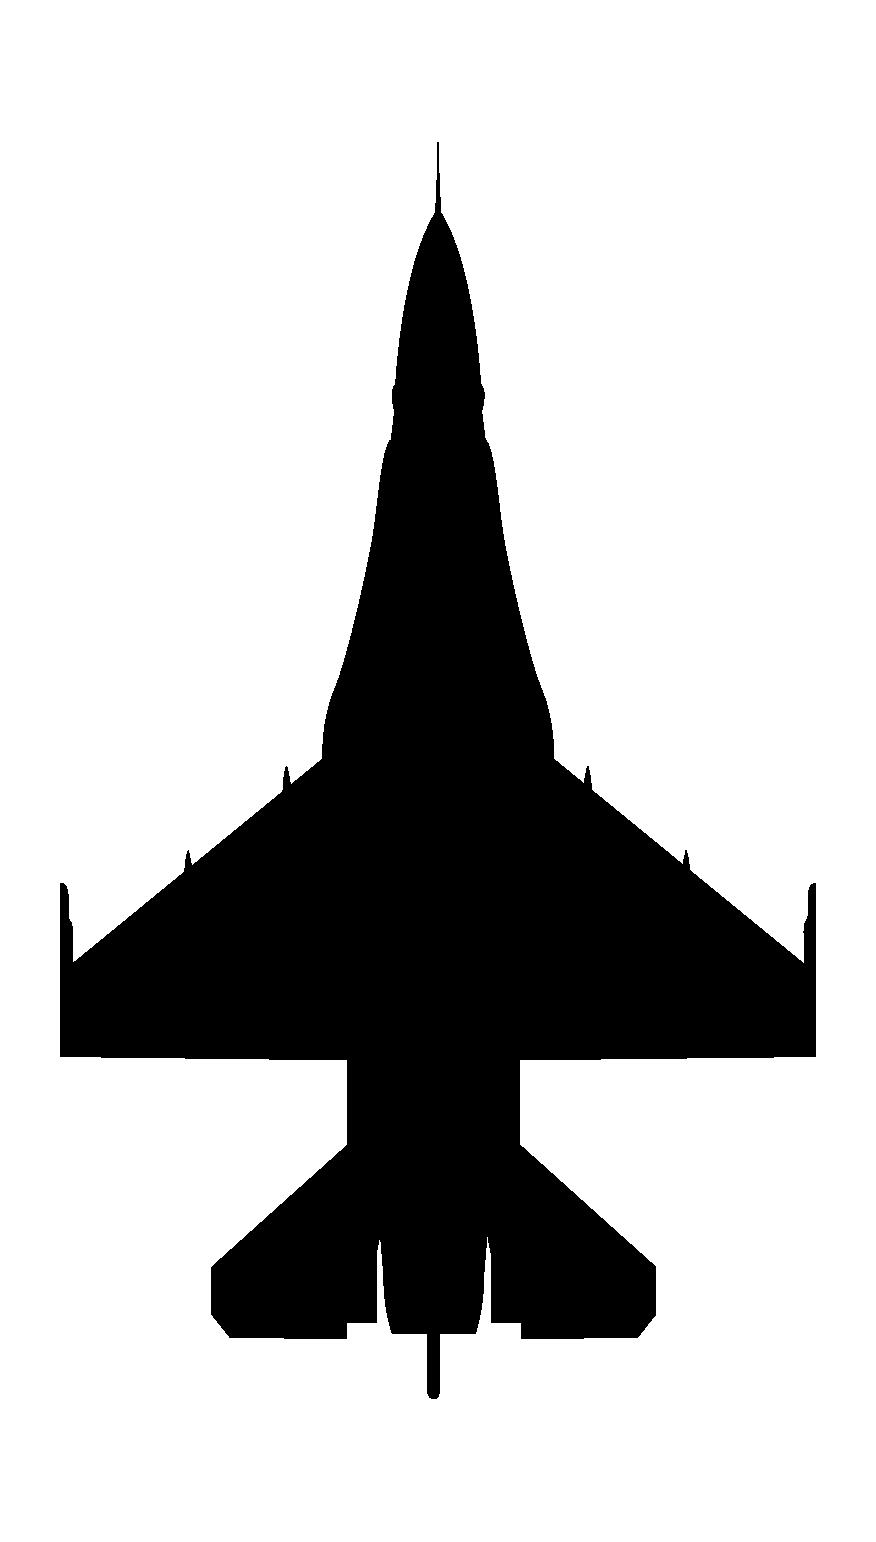
\includegraphics[
                width=7.5mm,
            ]{diagrams/aircraft/silhouette_f16_top.pdf}
        };
        
        \node[yshift=-3mm] (4fig) at (4) {
            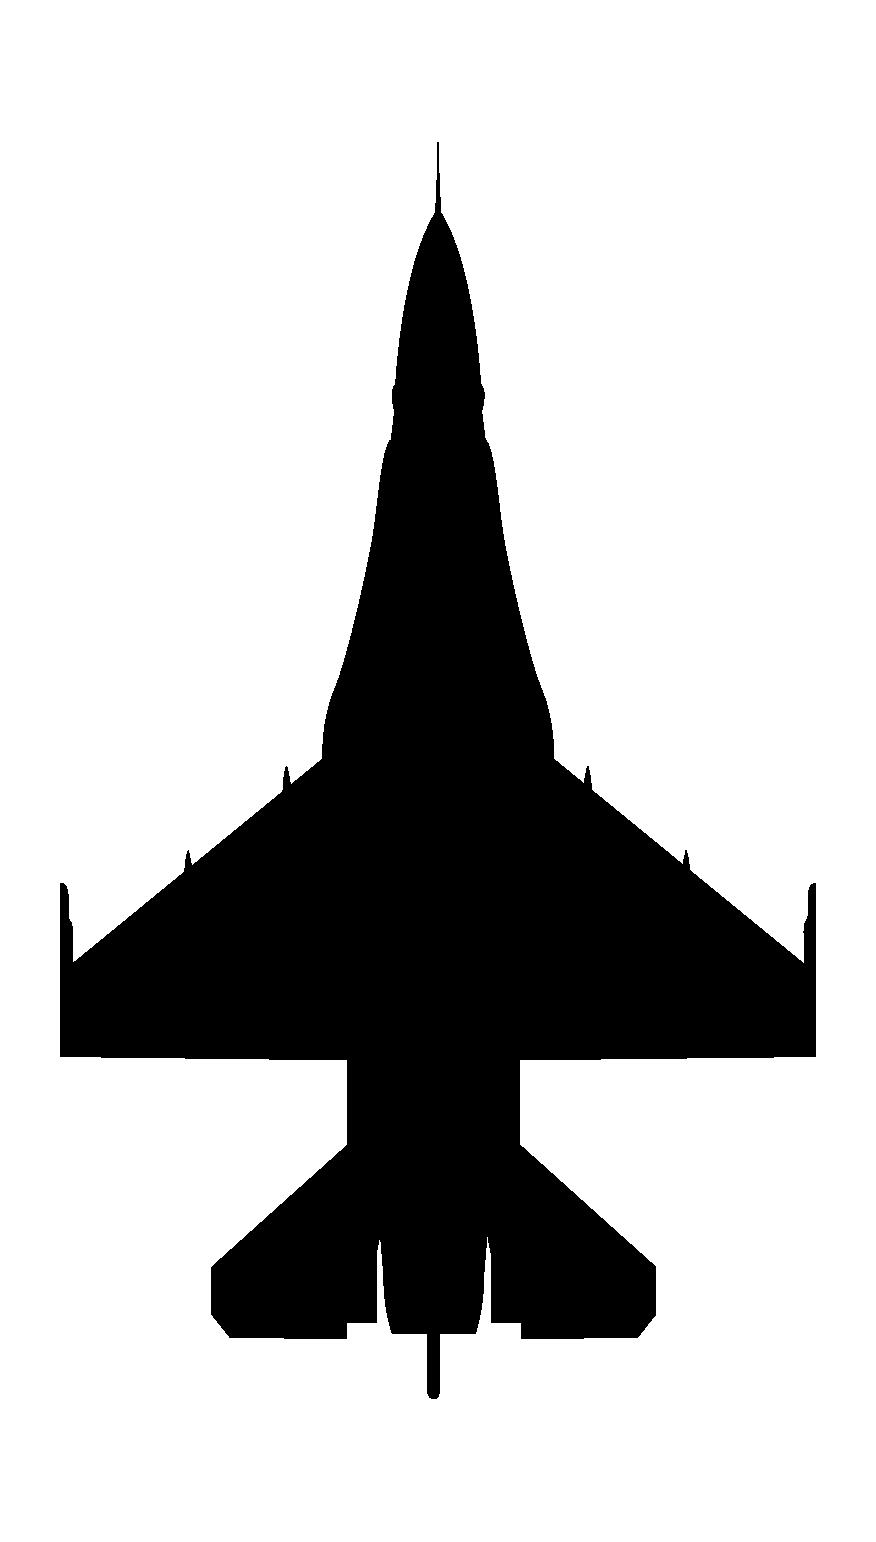
\includegraphics[
                width=7.5mm,
            ]{diagrams/aircraft/silhouette_f16_top.pdf}
        };

        \node[anchor=north, font=\footnotesize] (1label) at (1fig.south) {1};
        \node[anchor=north, font=\footnotesize] (3label) at (3fig.south) {3};

    \end{tikzpicture}
    \caption{Fluid Four}
    \label{fig:supp_fig:form:fluidfour}
\end{figure}

\paragraph{Res Cell} 
\textbf{Encumbers bandit radar sort}
--- wingmen hide within resolution cell of bandit radar

\medskip
\hfill\textbf{Reference \cref{fig:supp_fig:form:rescell}}

\paragraph{Box} 
\textbf{Staggered line abreast}
--- allows trailing element to cover lead element, trail can offset 

\medskip
\hfill\textbf{Reference \cref{fig:supp_fig:form:boxoffset}}

\paragraph{Diamond}
\textbf{Airshow formation}
--- no tactical advantage, hard to maintain,
you will die looking cool

\medskip
\hfill\textbf{Reference \cref{fig:supp_fig:form:diamond}}

\begin{figure}[htbp]
    \centering
    \begin{tikzpicture}[figstyle]
    
        \coordinate (1) at (0,0);
        \coordinate (2) at ($(1)+(210:10)$);
        \coordinate (3) at ($(1)+(0:20)$);
        \coordinate (4) at ($(3)+(-30:10)$);

        \draw[]
        (1) -- (2)
        node[font=\footnotesize, left, pos=1] {Fingertip};
        \draw[]
        (1) -- (3)
        node[font=\footnotesize, above, pos=0.5] {LAB};
        \draw[]
        (3) -- (4)
        node[font=\footnotesize, right, pos=1] {Fingertip};

        \node[yshift=-3mm] (1fig) at (1) {
            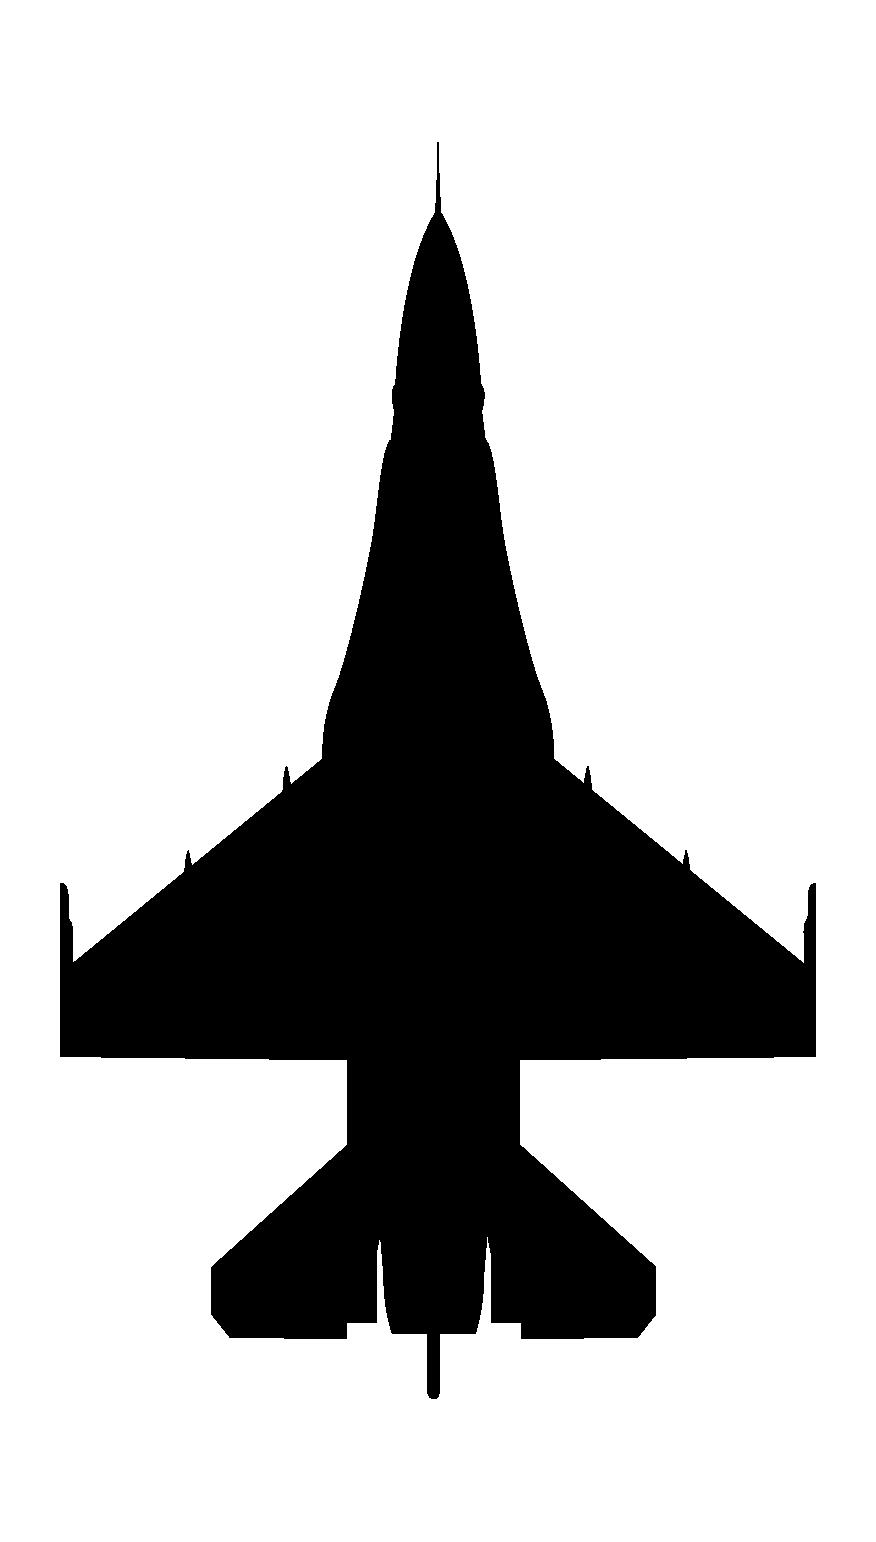
\includegraphics[
                width=7.5mm,
            ]{diagrams/aircraft/silhouette_f16_top.pdf}
        };
        
        \node[yshift=-3mm] (2fig) at (2) {
            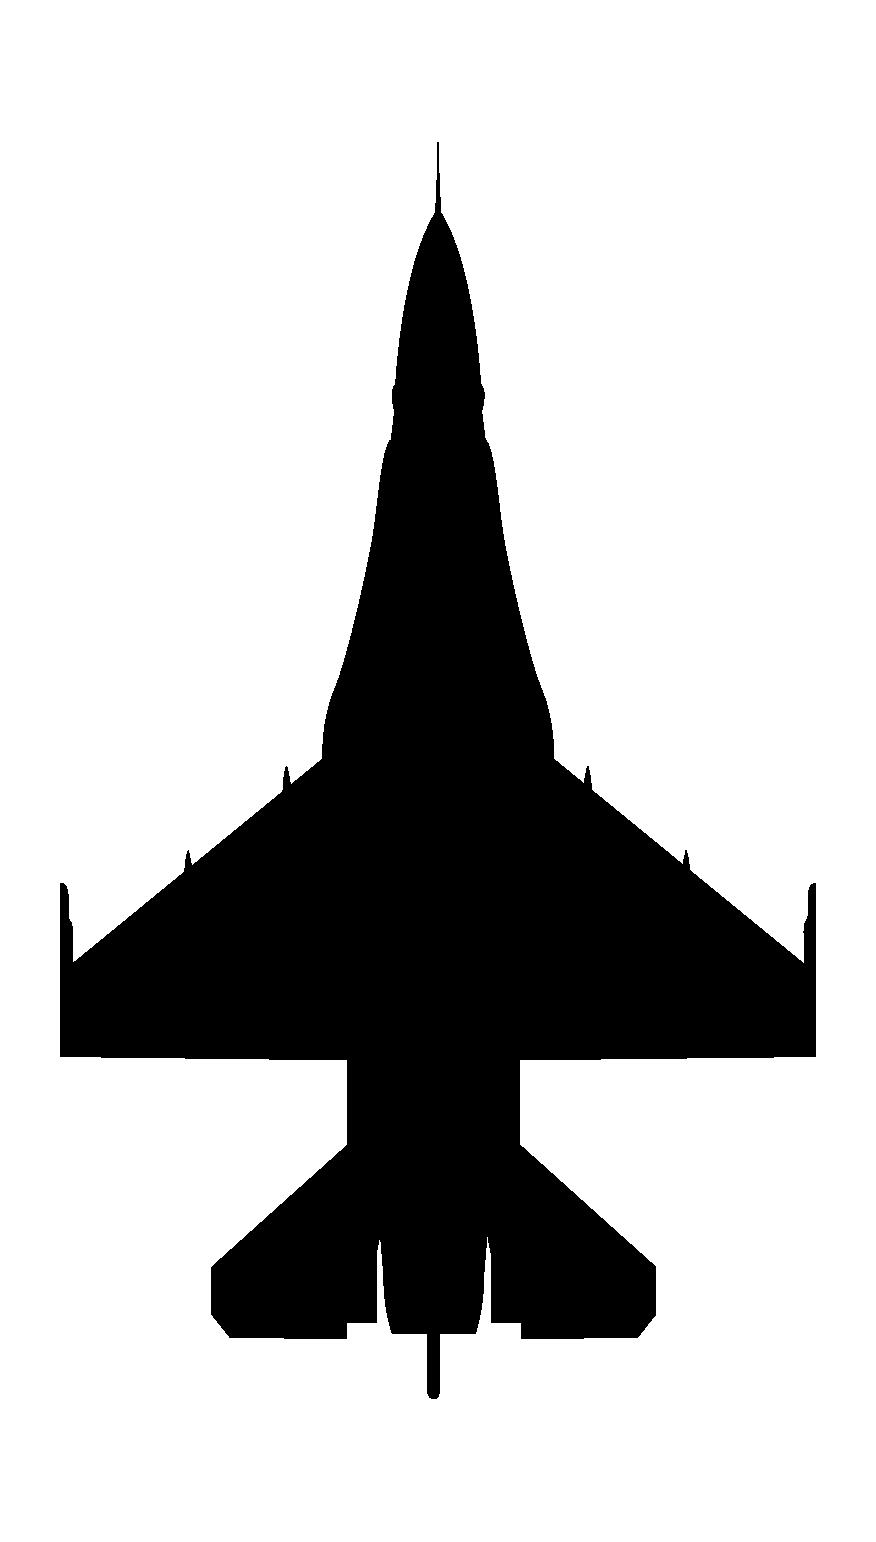
\includegraphics[
                width=7.5mm,
            ]{diagrams/aircraft/silhouette_f16_top.pdf}
        };

        \node[yshift=-3mm] (3fig) at (3) {
            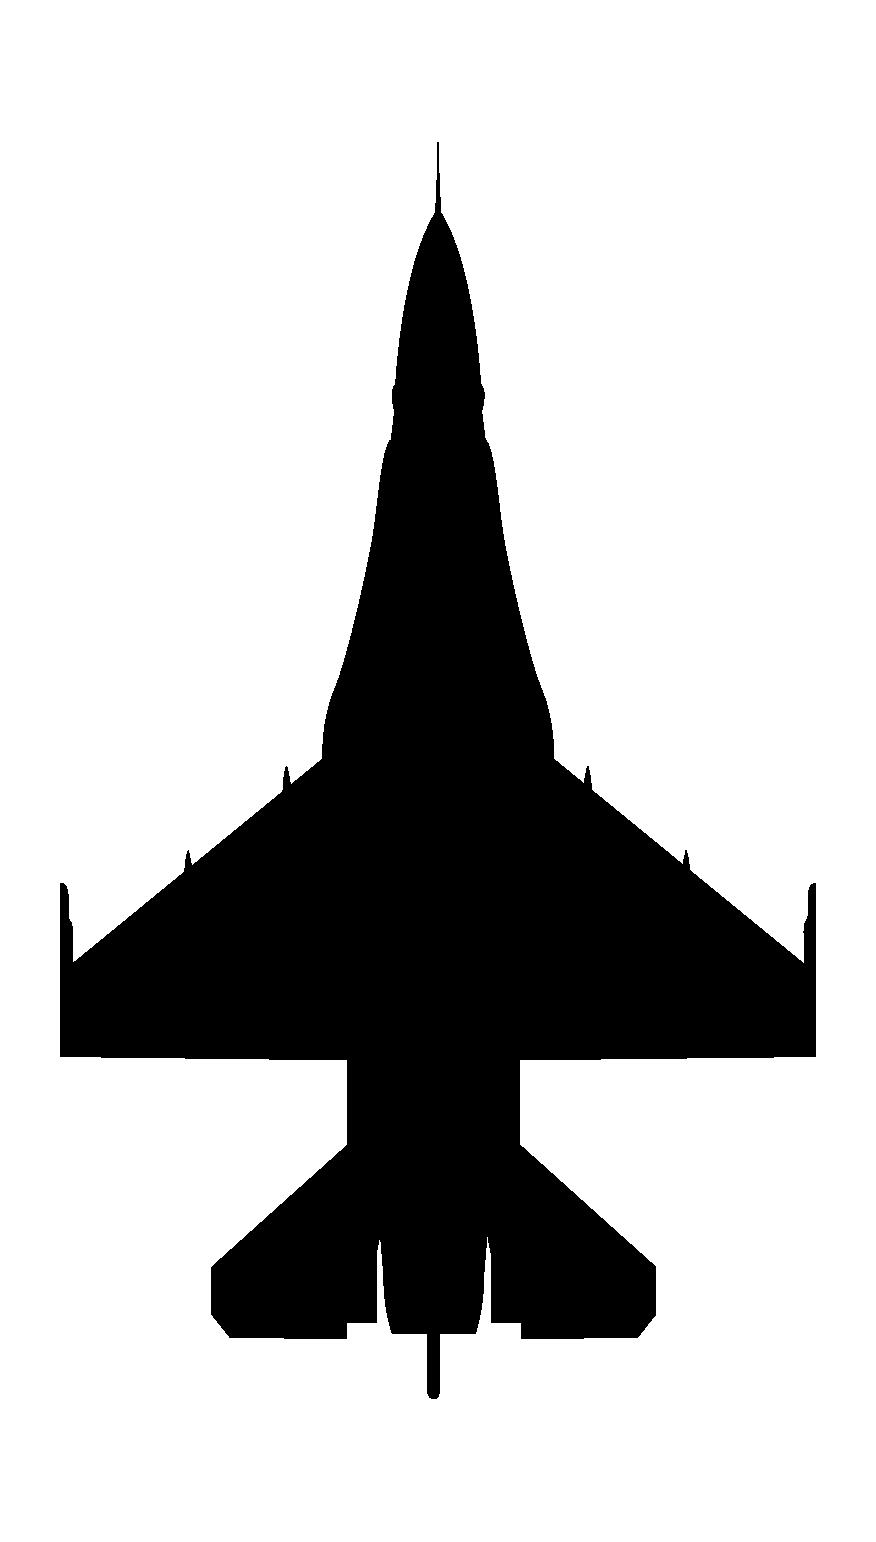
\includegraphics[
                width=7.5mm,
            ]{diagrams/aircraft/silhouette_f16_top.pdf}
        };
        
        \node[yshift=-3mm] (4fig) at (4) {
            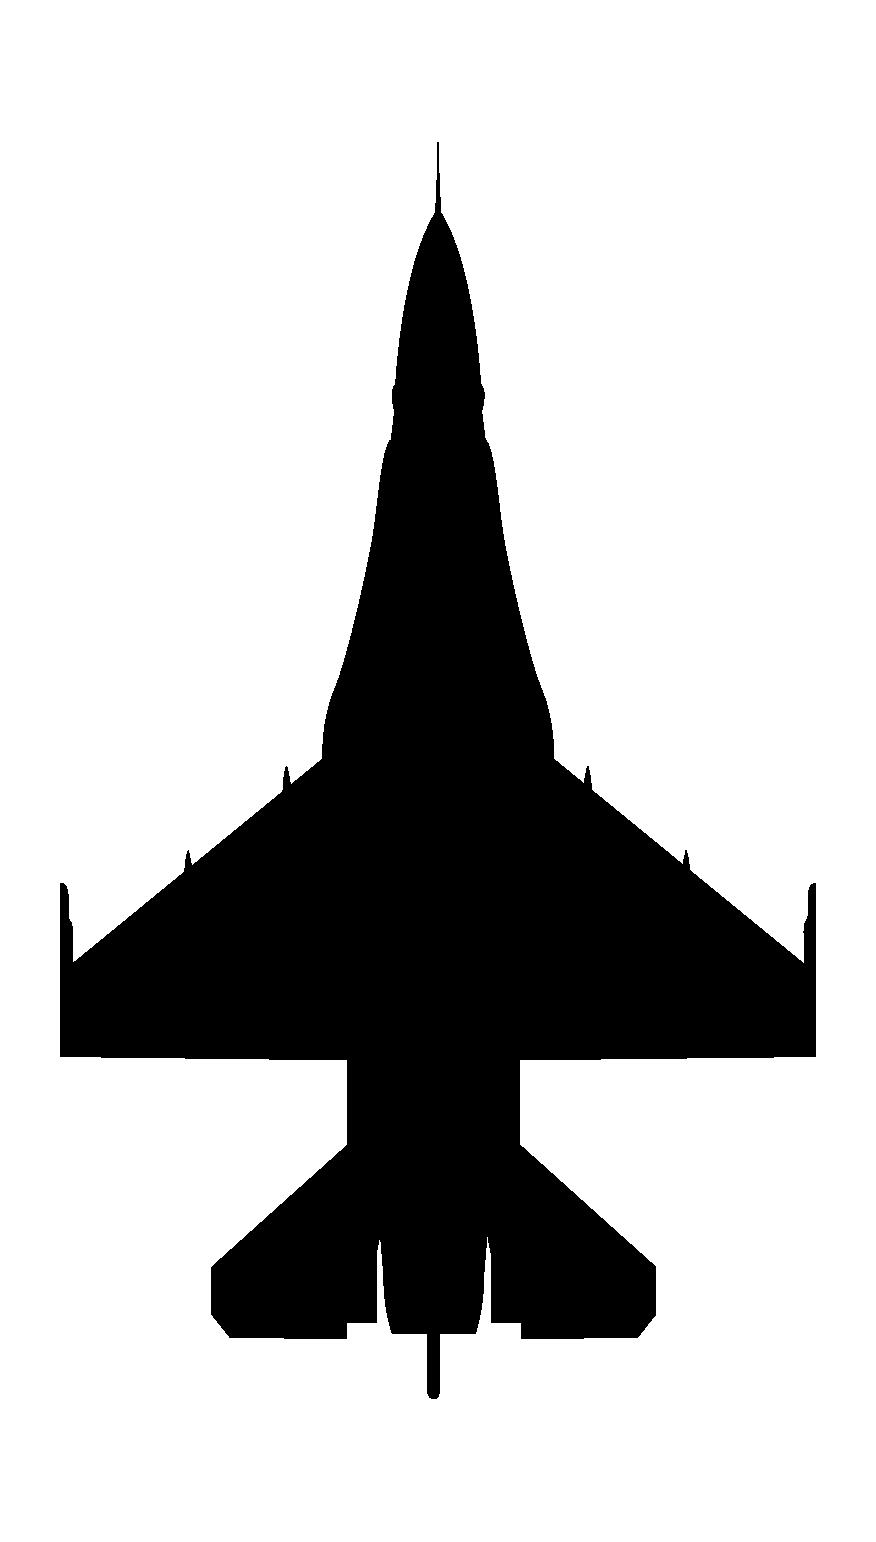
\includegraphics[
                width=7.5mm,
            ]{diagrams/aircraft/silhouette_f16_top.pdf}
        };

        \node[anchor=north, font=\footnotesize] (1label) at (1fig.south) {1};
        \node[anchor=north, font=\footnotesize] (2label) at (2fig.south) {2};
        \node[anchor=north, font=\footnotesize] (3label) at (3fig.south) {3};
        \node[anchor=north, font=\footnotesize] (4label) at (4fig.south) {4};

    \end{tikzpicture}
    \caption{Res Cell}
    \label{fig:supp_fig:form:rescell}
\end{figure}

\begin{figure}[htbp]
    \centering
    \begin{minipage}[b]{0.5\textwidth}
        \centering
        \begin{tikzpicture}[figstyle]
            
            \coordinate (1) at (0,0);
            \coordinate (2) at ($(1)+(20,0)$);
            \coordinate (3) at ($(1)+(10,-30)$);
            \coordinate (4) at ($(3)+(20,0)$);

            \draw[<->]
            ($(1)+(-5,0)$) 
            -- ($(3)+(-15,0)$)
            node[font=\footnotesize, pos=0.5, rotate=90, above] {1.5-3.0 nm};
            \draw[thin]
            (1) -- ($(1)+(-7,0)$)
            (3) -- ($(3)+(-17,0)$);

            \draw[]
            (1) -- (2)
            node[font=\footnotesize, pos=0.5, above] {LAB};

            \draw[]
            (3) -- (4)
            node[font=\footnotesize, pos=0.5, above] {LAB};


            \node[yshift=-2mm] (1fig) at (1) {
                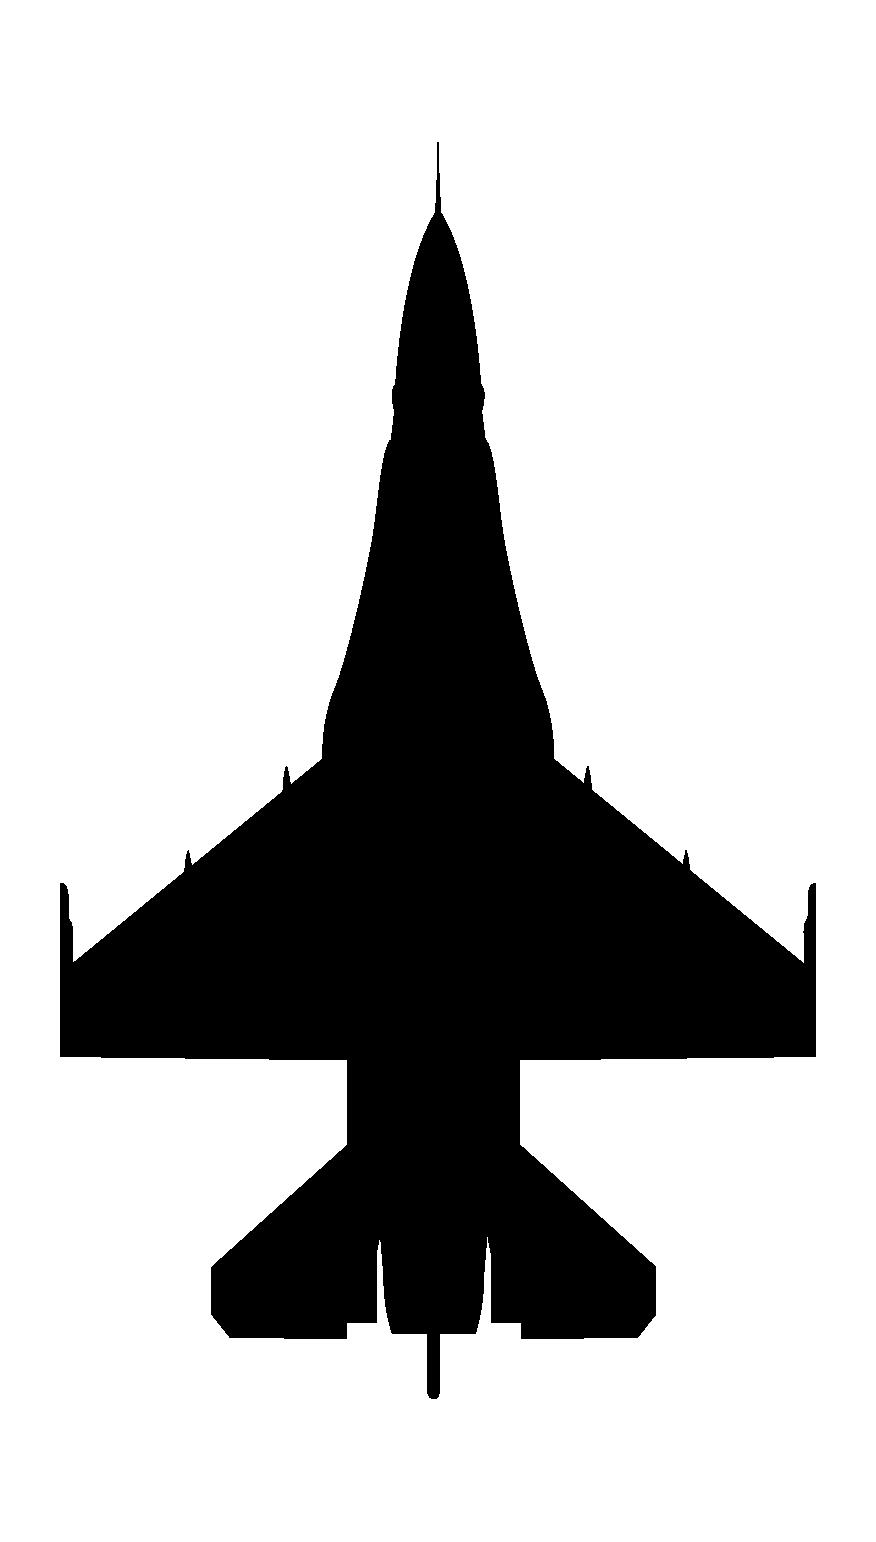
\includegraphics[
                    width=7.5mm,
                ]{diagrams/aircraft/silhouette_f16_top.pdf}
            };
            
            \node[yshift=-2mm] (2fig) at (2) {
                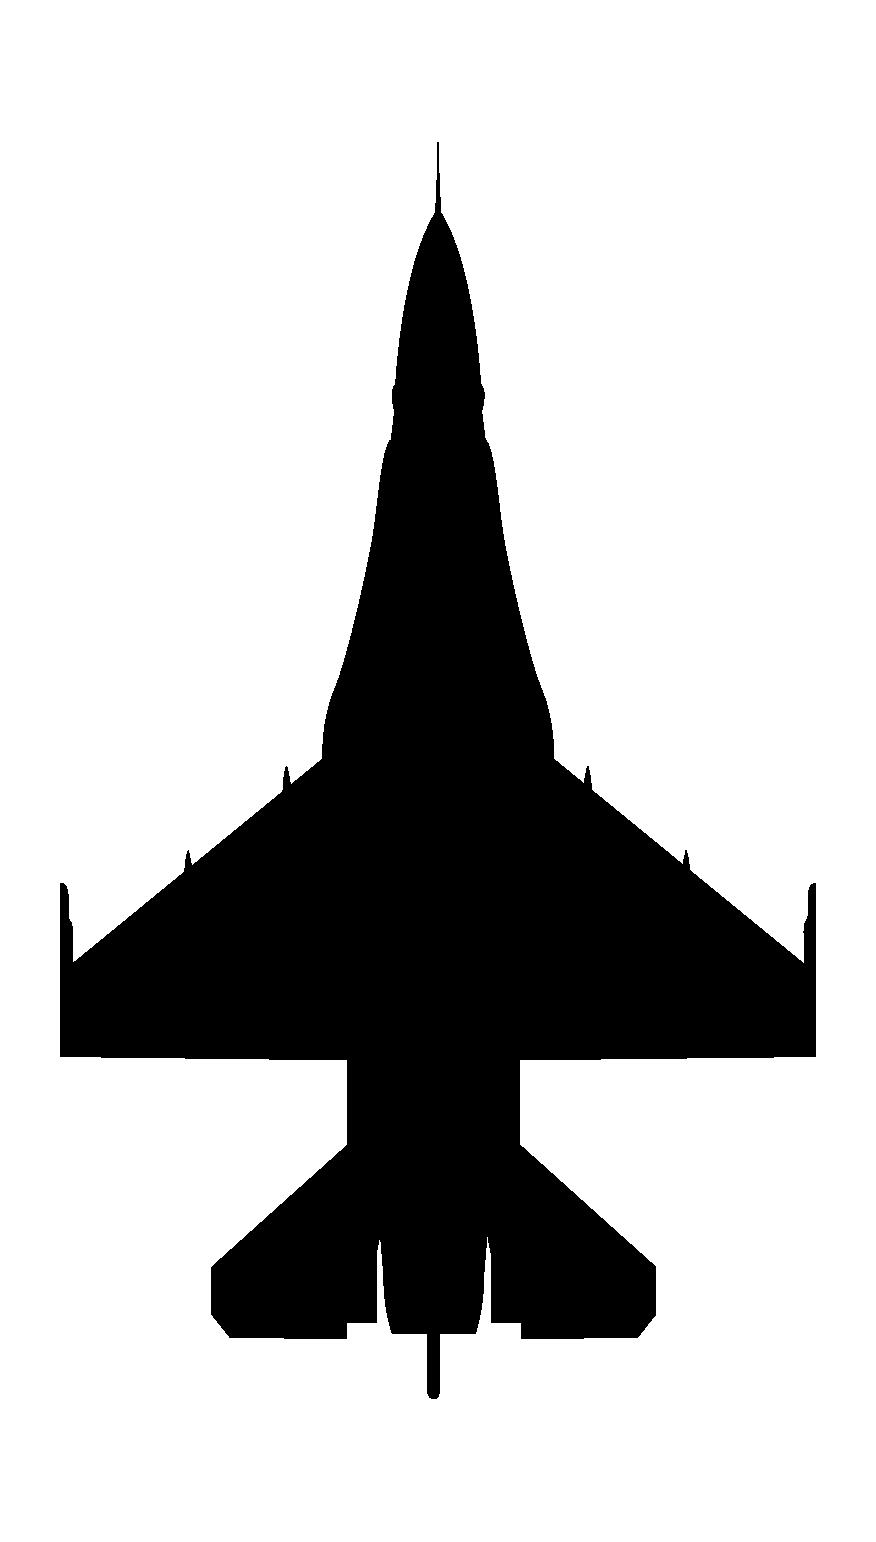
\includegraphics[
                    width=7.5mm,
                ]{diagrams/aircraft/silhouette_f16_top.pdf}
            };

            \node[yshift=-2mm] (3fig) at (3) {
                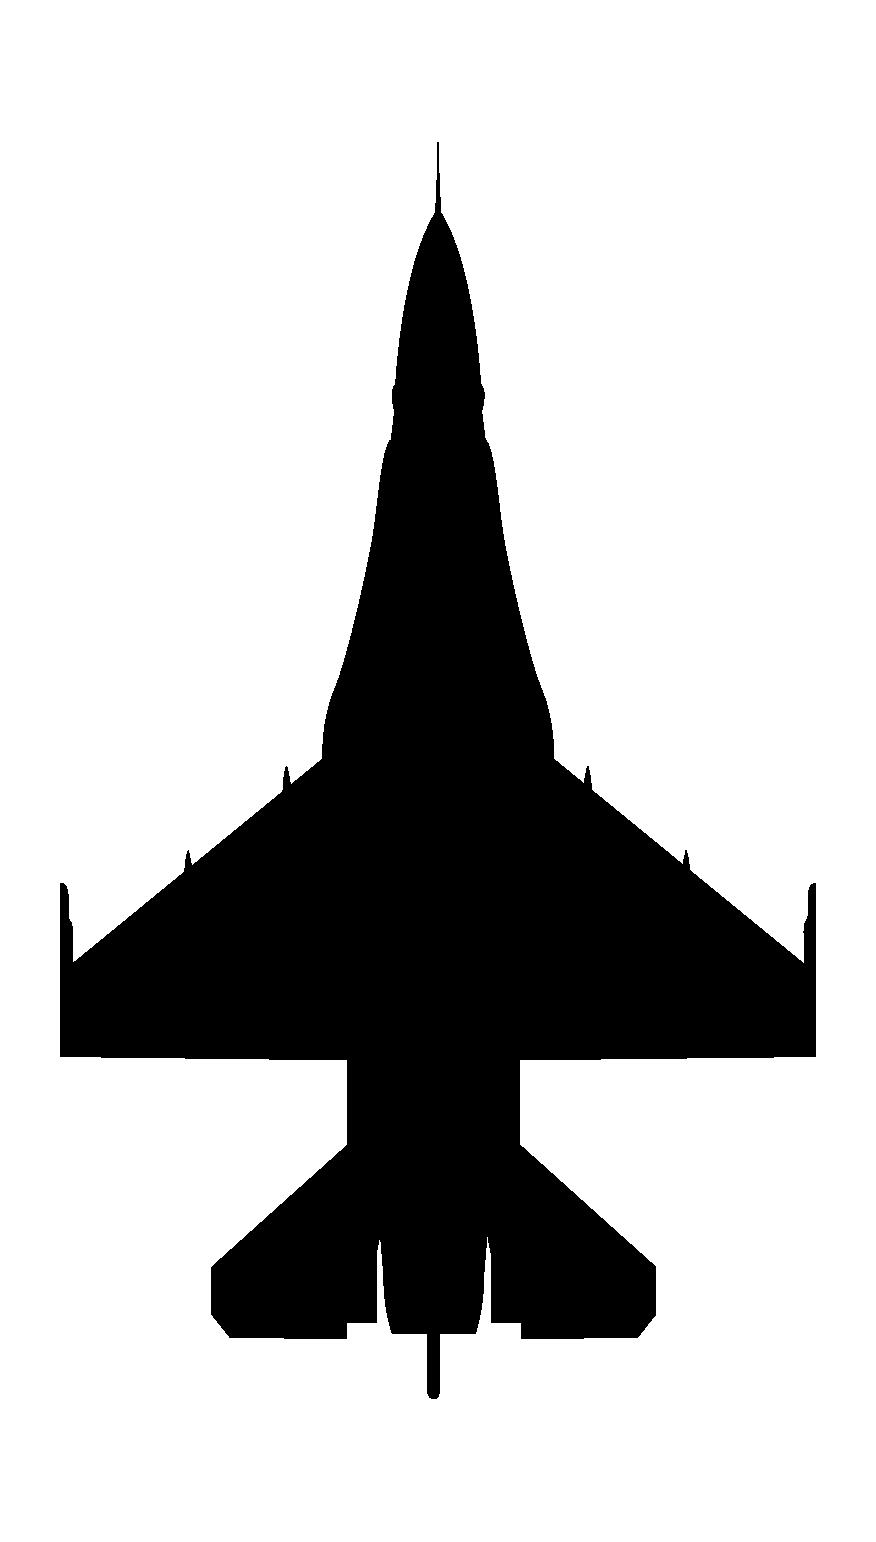
\includegraphics[
                    width=7.5mm,
                ]{diagrams/aircraft/silhouette_f16_top.pdf}
            };
            
            \node[yshift=-2mm] (4fig) at (4) {
                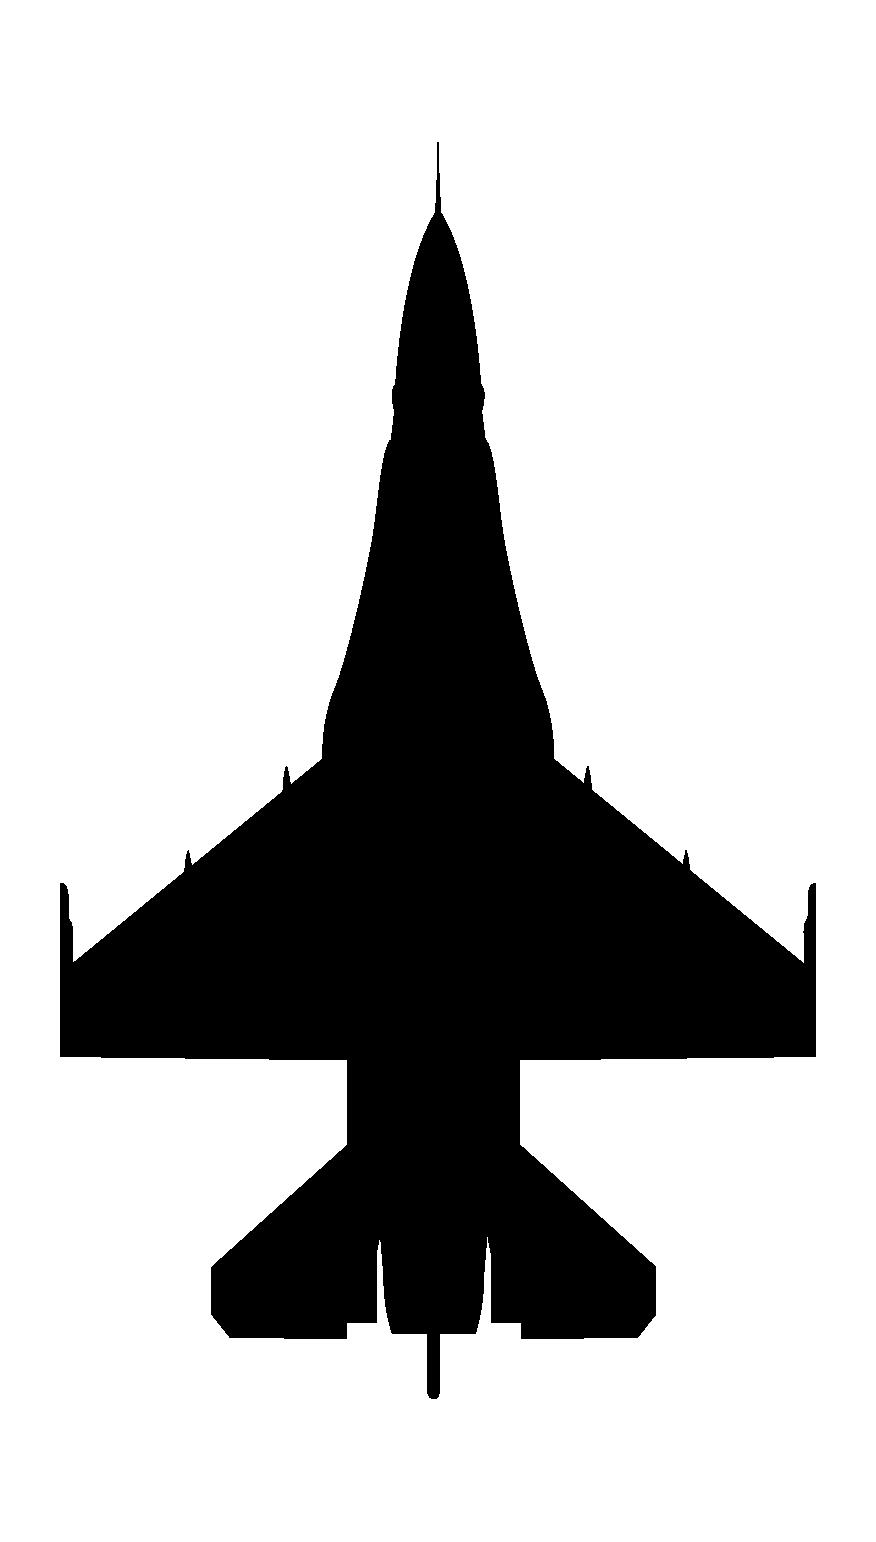
\includegraphics[
                    width=7.5mm,
                ]{diagrams/aircraft/silhouette_f16_top.pdf}
            };

            \node[anchor=north, font=\footnotesize] (1label) at (1fig.south) {1};
            \node[anchor=north, font=\footnotesize] (2label) at (2fig.south) {2};
            \node[anchor=north, font=\footnotesize] (3label) at (3fig.south) {3};
            \node[anchor=north, font=\footnotesize] (4label) at (4fig.south) {4};

        \end{tikzpicture}
        \caption{Four-ship offset box}
        \label{fig:supp_fig:form:boxoffset}
    \end{minipage}%
    \begin{minipage}[b]{0.5\textwidth}
        \centering
        \begin{tikzpicture}[figstyle]
            
            \coordinate (1) at (0,0);
            \coordinate (2) at ($(1)+(-135:10)$);
            \coordinate (3) at ($(1)+(-45:10)$);
            \coordinate (4) at ($(3)+(-135:10)$);

            \node[yshift=-2mm] (1fig) at (1) {
                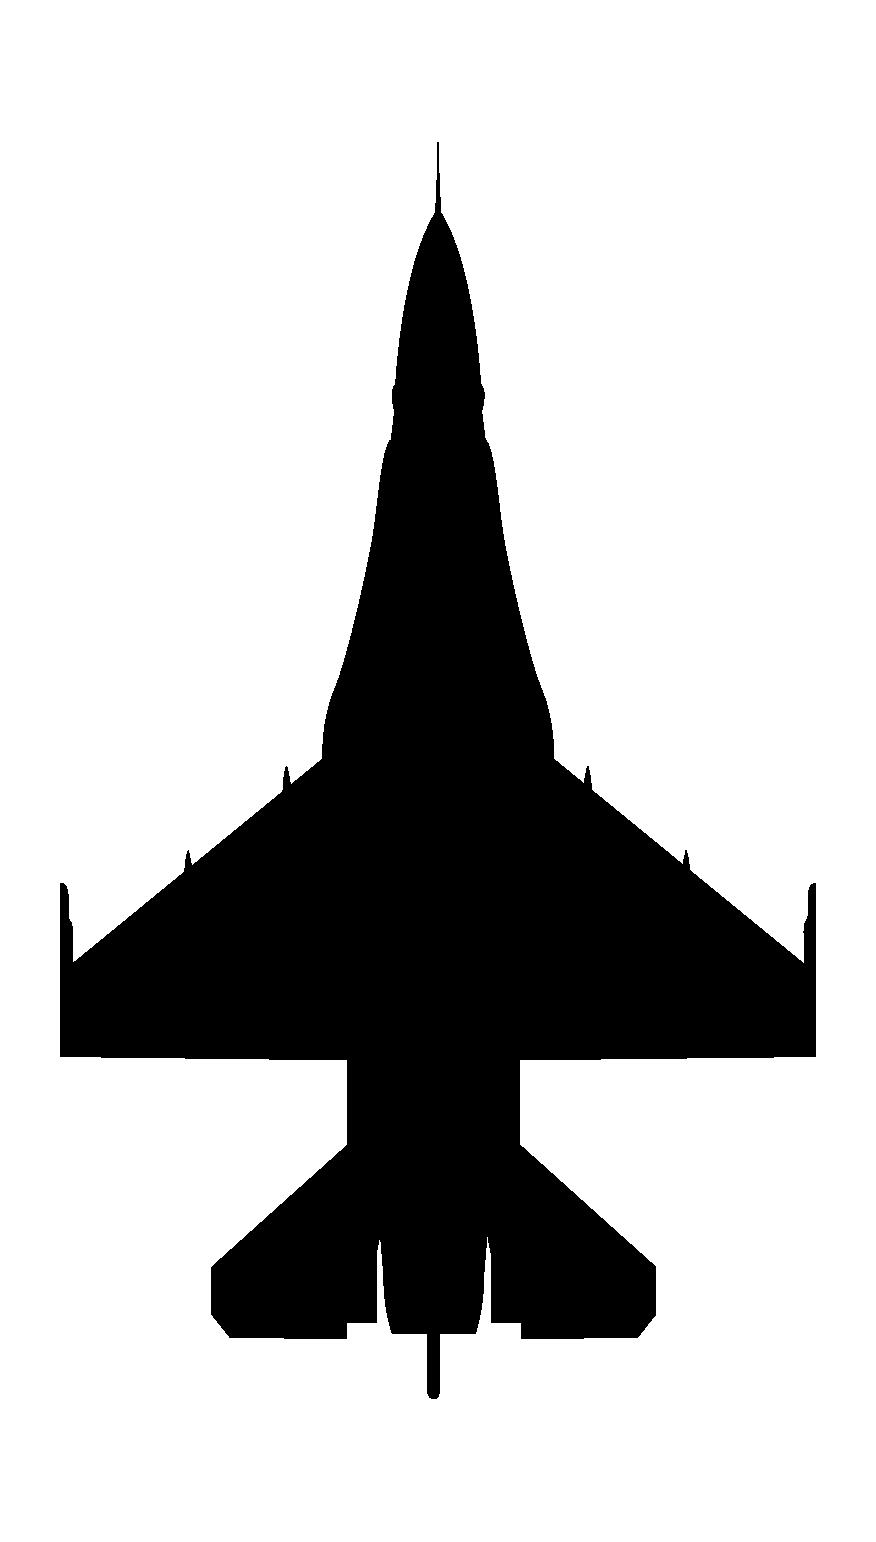
\includegraphics[
                    width=7.5mm,
                ]{diagrams/aircraft/silhouette_f16_top.pdf}
            };
            
            \node[yshift=-2mm] (2fig) at (2) {
                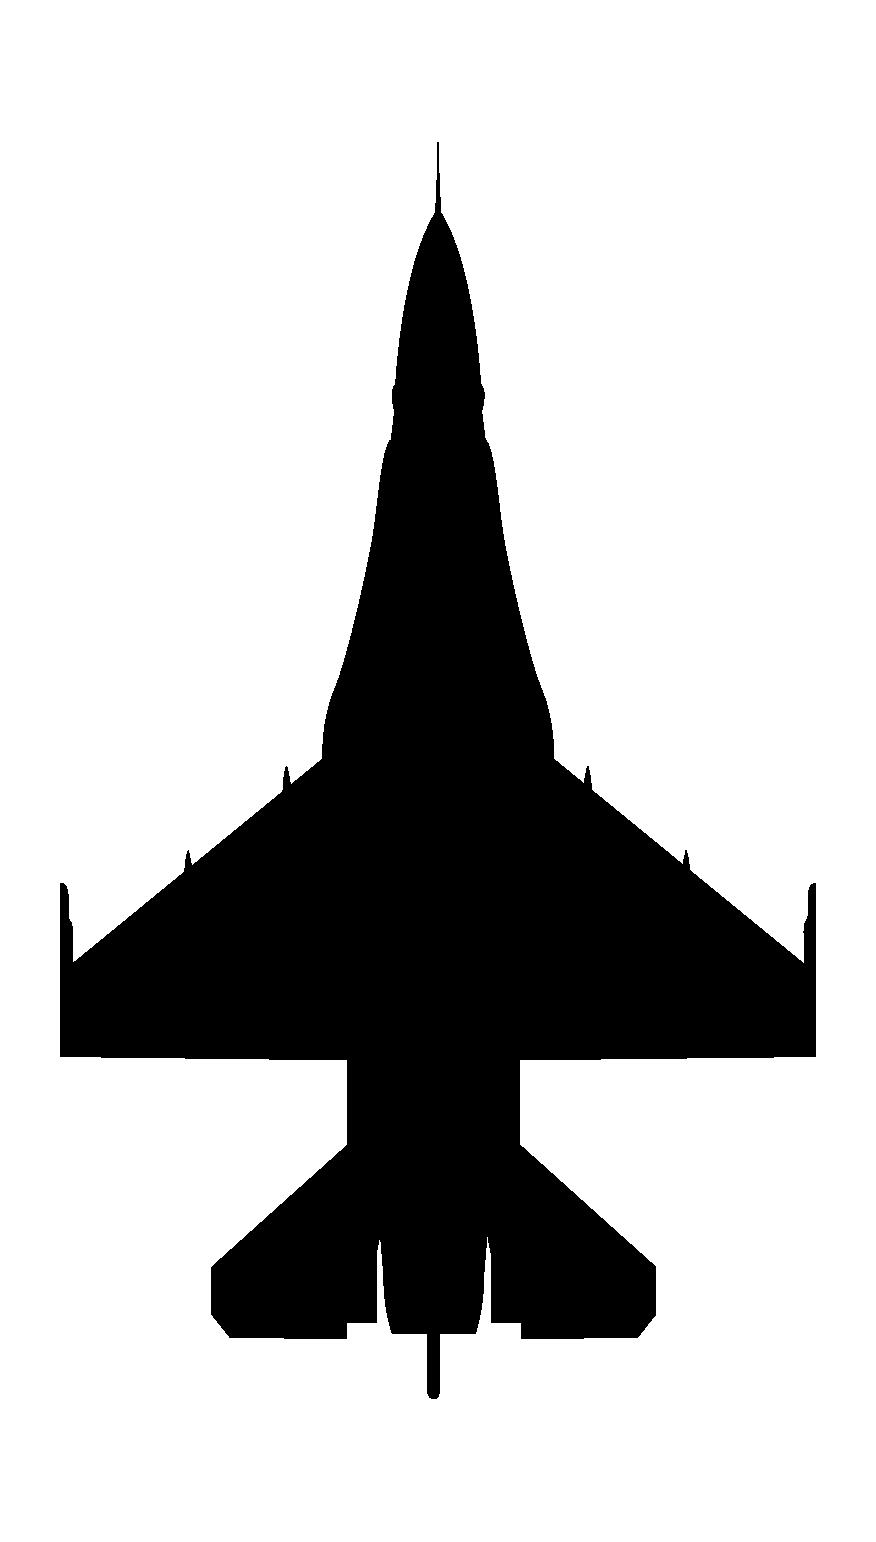
\includegraphics[
                    width=7.5mm,
                ]{diagrams/aircraft/silhouette_f16_top.pdf}
            };

            \node[yshift=-2mm] (3fig) at (3) {
                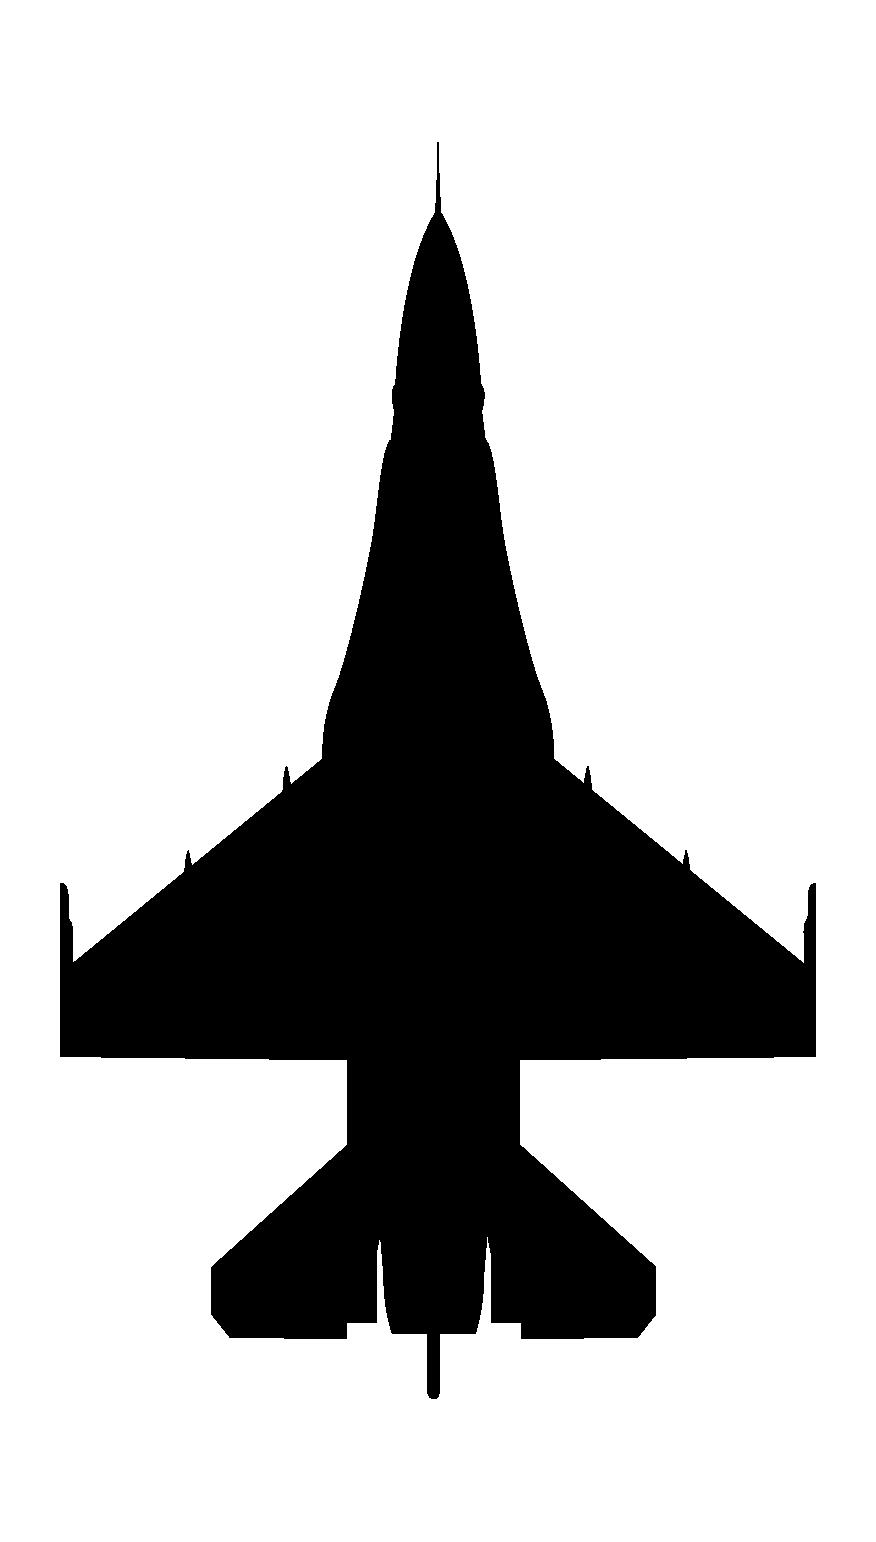
\includegraphics[
                    width=7.5mm,
                ]{diagrams/aircraft/silhouette_f16_top.pdf}
            };
            
            \node[yshift=-2mm] (4fig) at (4) {
                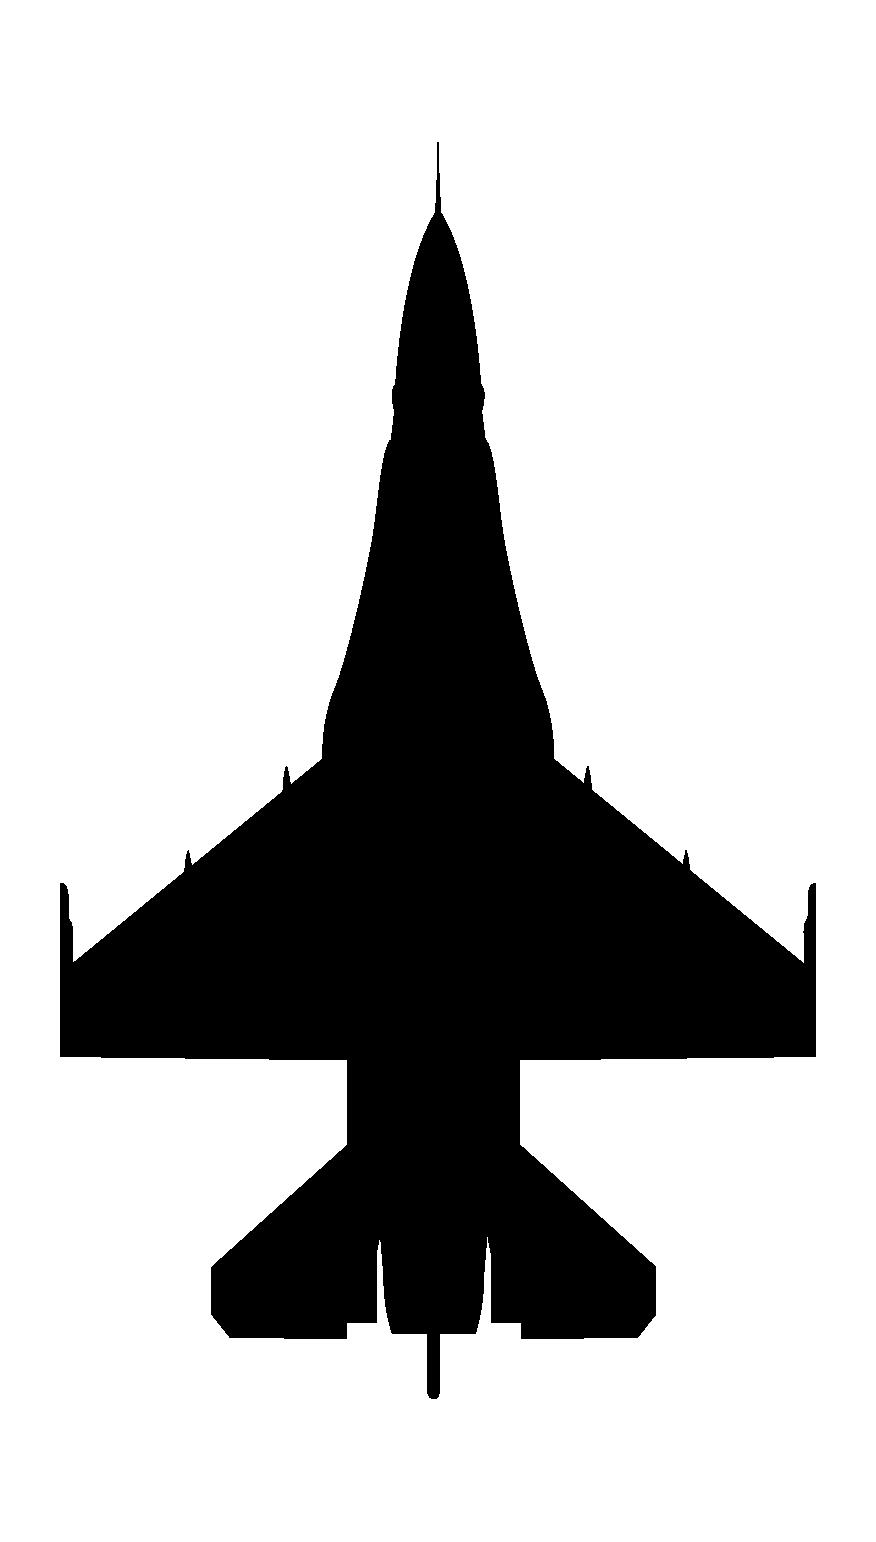
\includegraphics[
                    width=7.5mm,
                ]{diagrams/aircraft/silhouette_f16_top.pdf}
            };

            \node[anchor=south, font=\footnotesize] (1label) at (1fig.north) {1};
            \node[anchor=north, font=\footnotesize] (2label) at (2fig.south) {2};
            \node[anchor=north, font=\footnotesize] (3label) at (3fig.south) {3};
            \node[anchor=north, font=\footnotesize] (4label) at (4fig.south) {4};

        \end{tikzpicture}
        \caption{Diamond}
        \label{fig:supp_fig:form:diamond}
    \end{minipage}
\end{figure}

\clearpage

\paragraph{Trail} 
\textbf{IFR formation}
--- allows radar / TACAN contact between flight members for deconfliction,
distance as briefed

\medskip
\hfill\textbf{Reference \cref{fig:supp_fig:form:trail}}

\paragraph{Stack}
\textbf{More restrictive trail} --- similar to trail but with altitude separation and tighter distance constraints

\medskip
\hfill\textbf{Reference \cref{fig:supp_fig:form:stack}}

\paragraph{Ladder}
\textbf{A-G formation}
--- similar to trail but with altitude separation

\medskip
\hfill\textbf{Reference \cref{fig:supp_fig:form:ladder}}

\begin{figure}[htbp]
    \centering
    \begin{tikzpicture}[figstyle]
        
        \coordinate (1) at (0,0);
        \coordinate (2) at ($(1)+(180:20)$);
        \coordinate (3) at ($(2)+(180:20)$);
        \coordinate (4) at ($(3)+(180:20)$);

        \node[yshift=-2mm, rotate=-90] (1fig) at (1) {
            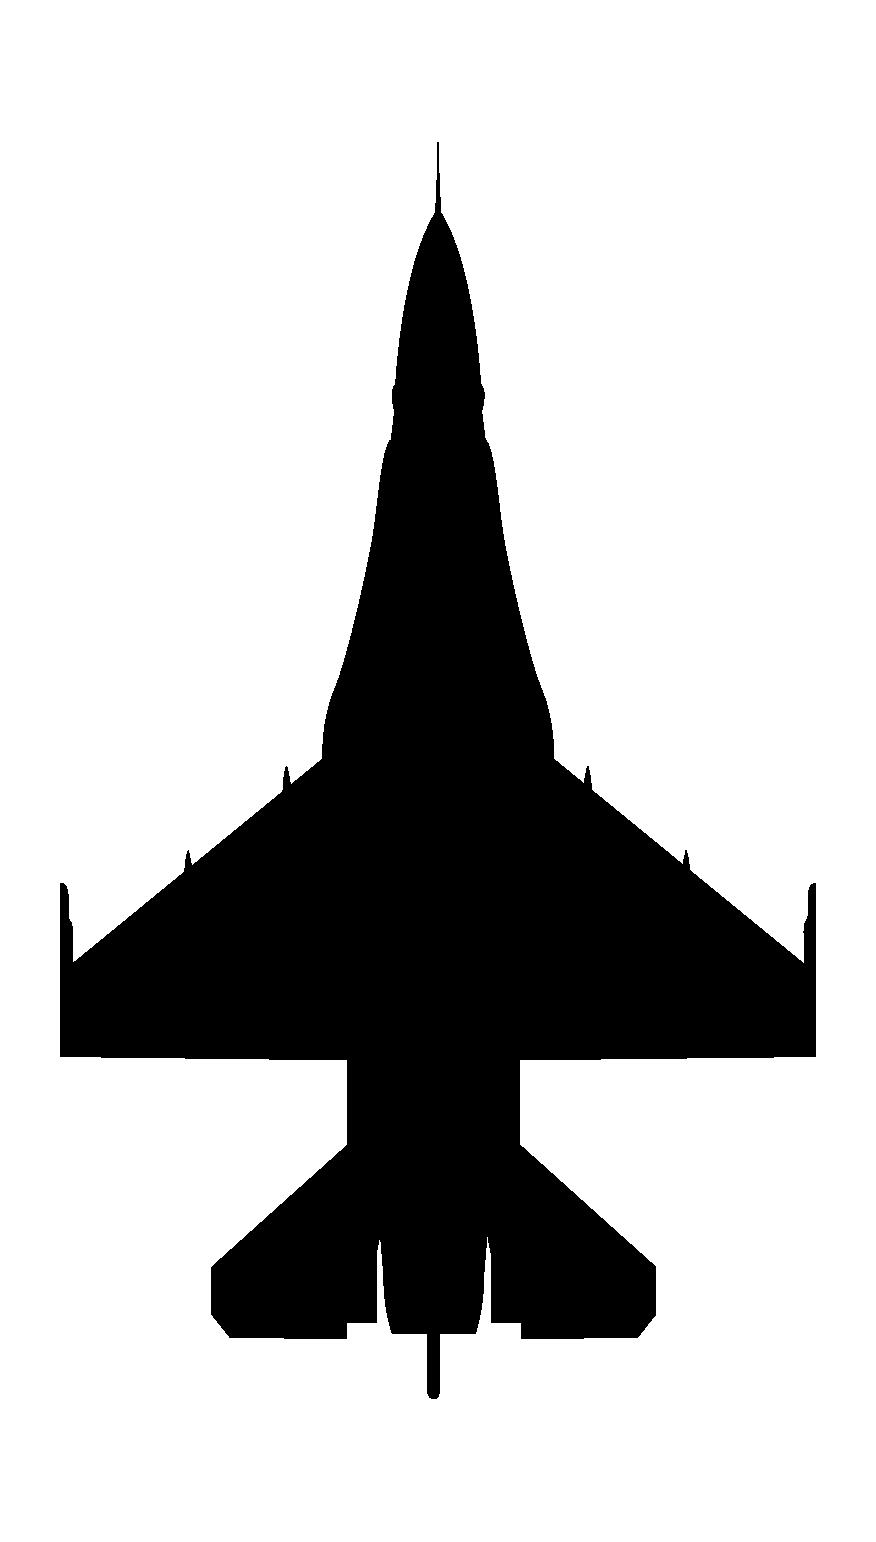
\includegraphics[
                width=7.5mm,
            ]{diagrams/aircraft/silhouette_f16_top.pdf}
        };
        
        \node[yshift=-2mm, rotate=-90] (2fig) at (2) {
            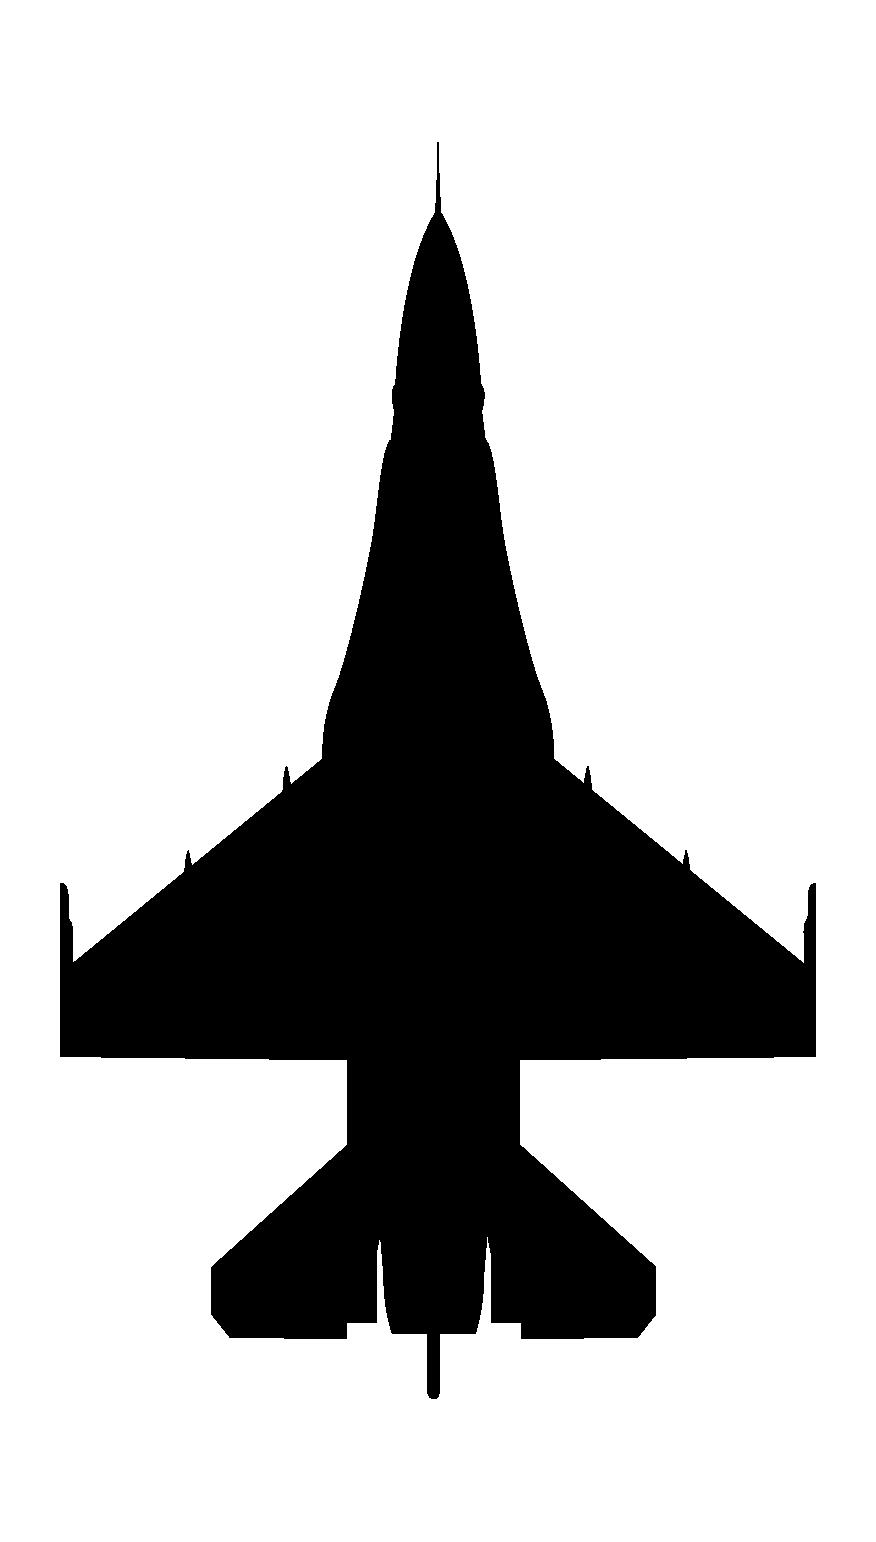
\includegraphics[
                width=7.5mm,
            ]{diagrams/aircraft/silhouette_f16_top.pdf}
        };

        \node[yshift=-2mm, rotate=-90] (3fig) at (3) {
            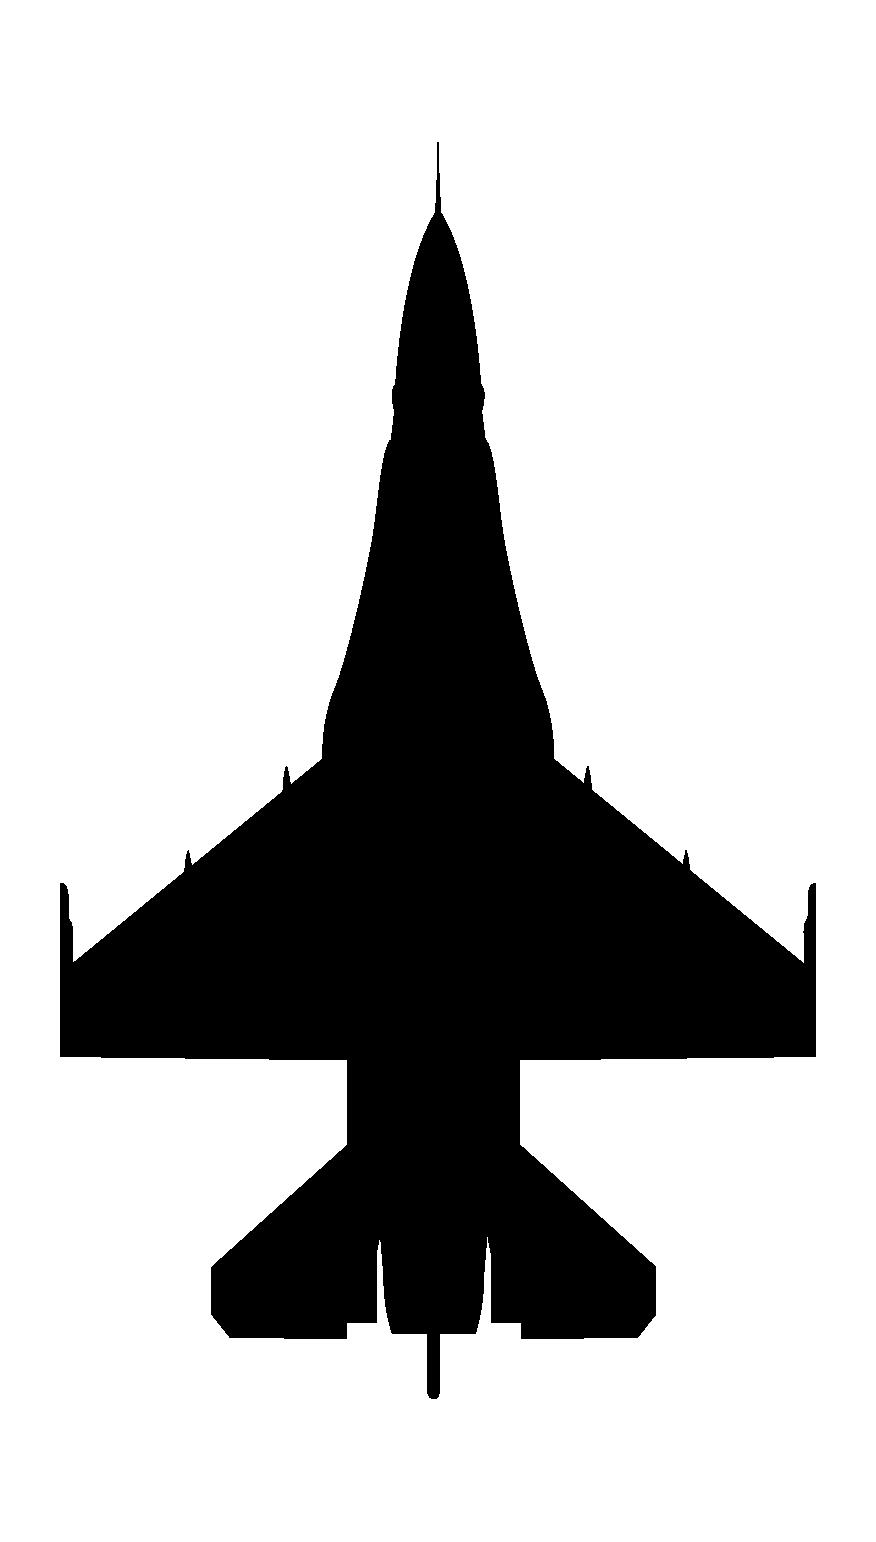
\includegraphics[
                width=7.5mm,
            ]{diagrams/aircraft/silhouette_f16_top.pdf}
        };
        
        \node[yshift=-2mm, rotate=-90] (4fig) at (4) {
            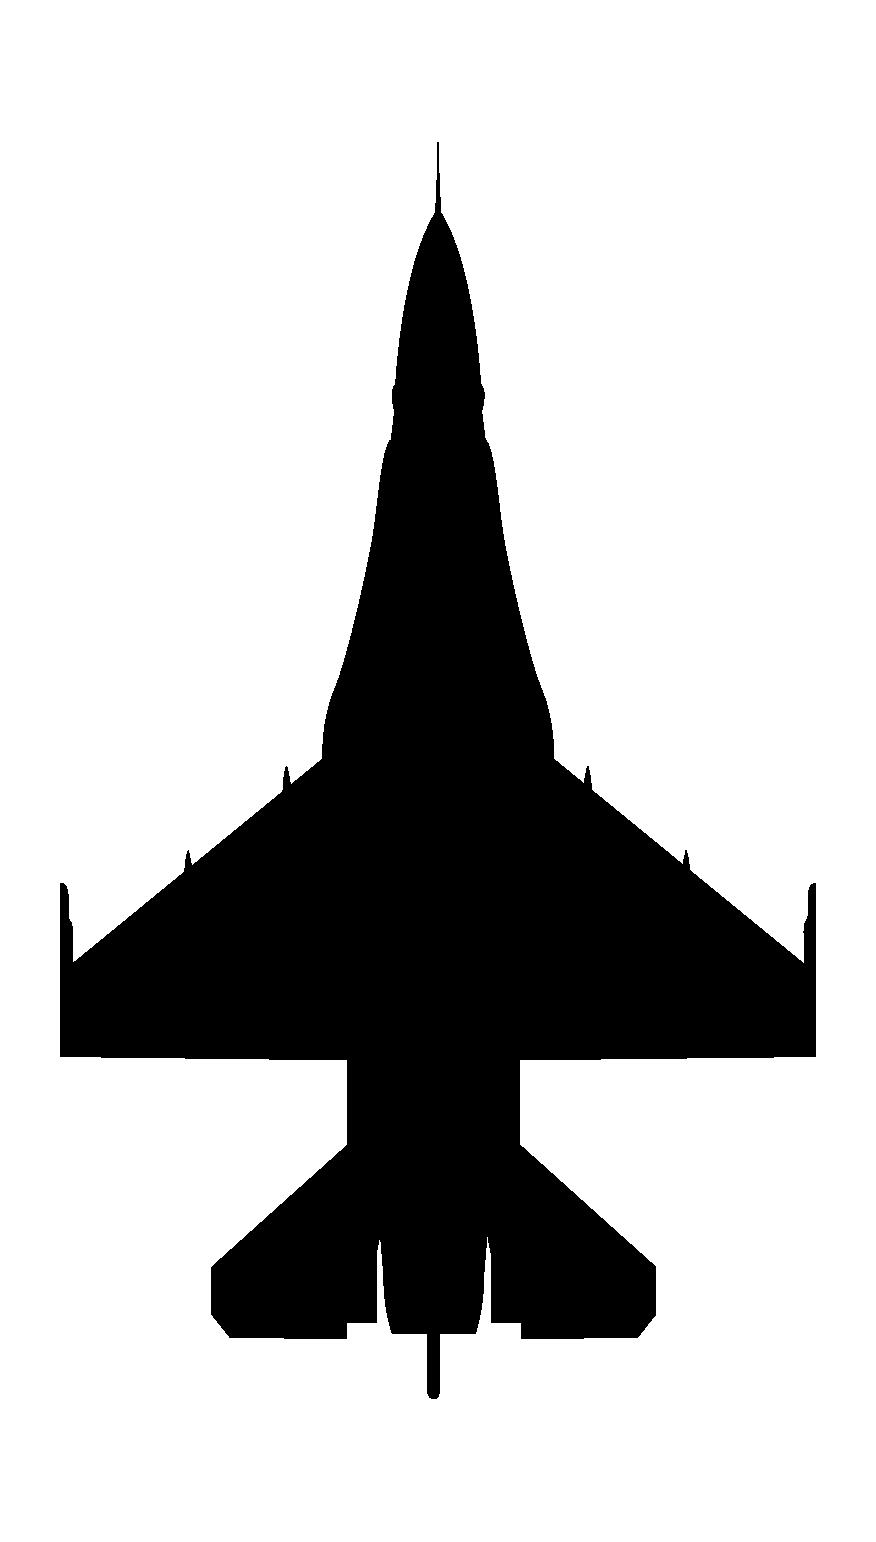
\includegraphics[
                width=7.5mm,
            ]{diagrams/aircraft/silhouette_f16_top.pdf}
        };

        \node[anchor=north, font=\footnotesize] (1label) at (1fig.east) {1};
        \node[anchor=north, font=\footnotesize] (2label) at (2fig.east) {2};
        \node[anchor=north, font=\footnotesize] (3label) at (3fig.east) {3};
        \node[anchor=north, font=\footnotesize] (4label) at (4fig.east) {4};

    \end{tikzpicture}
    \caption{Trail}
    \label{fig:supp_fig:form:trail}
\end{figure}

\begin{figure}[htbp]
    \centering
    \begin{tikzpicture}[figstyle]
        
        \coordinate (1) at (0,0);
        \coordinate (2) at ($(1)+(-20, -5)$);
        \coordinate (3) at ($(2)+(-20, -5)$);
        \coordinate (4) at ($(3)+(-20, -5)$);

        \draw[<->, thin]
        ($(2)+(10,0)$) 
        -- ($(3)+(30,0)$)
        node[font=\footnotesize, pos=0.5, right] {500-2000 ft};
        \draw[thin]
        (2) -- ($(2)+(12,0)$)
        (3) -- ($(3)+(32,0)$);

        \draw[<->, thin]
        ($(3)+(0,10)$) 
        -- ($(4)+(0,15)$)
        node[font=\footnotesize, pos=0.5, above] {0.5-1.0 nm};
        \draw[thin]
        (3) -- ($(3)+(0,12)$)
        (4) -- ($(4)+(0,17)$);

        \node[yshift=0.75mm] (1fig) at (1) {
            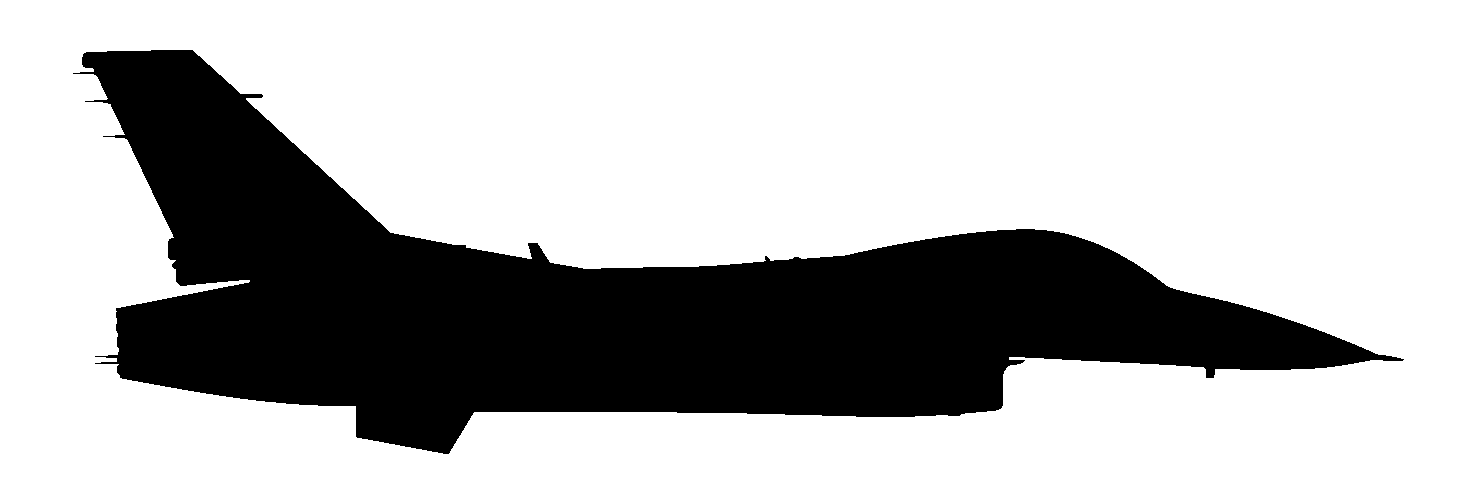
\includegraphics[
                width=12mm,
            ]{diagrams/aircraft/silhouette_f16_side.pdf}
        };
        
        \node[yshift=0.75mm] (2fig) at (2) {
            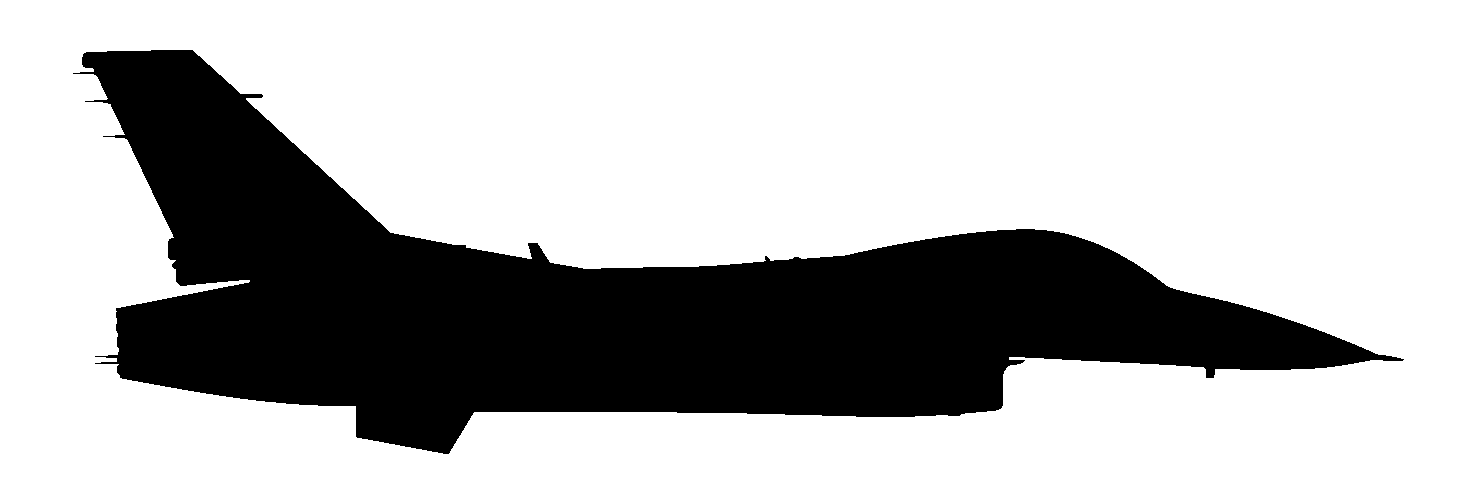
\includegraphics[
                width=12mm,
            ]{diagrams/aircraft/silhouette_f16_side.pdf}
        };

        \node[yshift=0.75mm] (3fig) at (3) {
            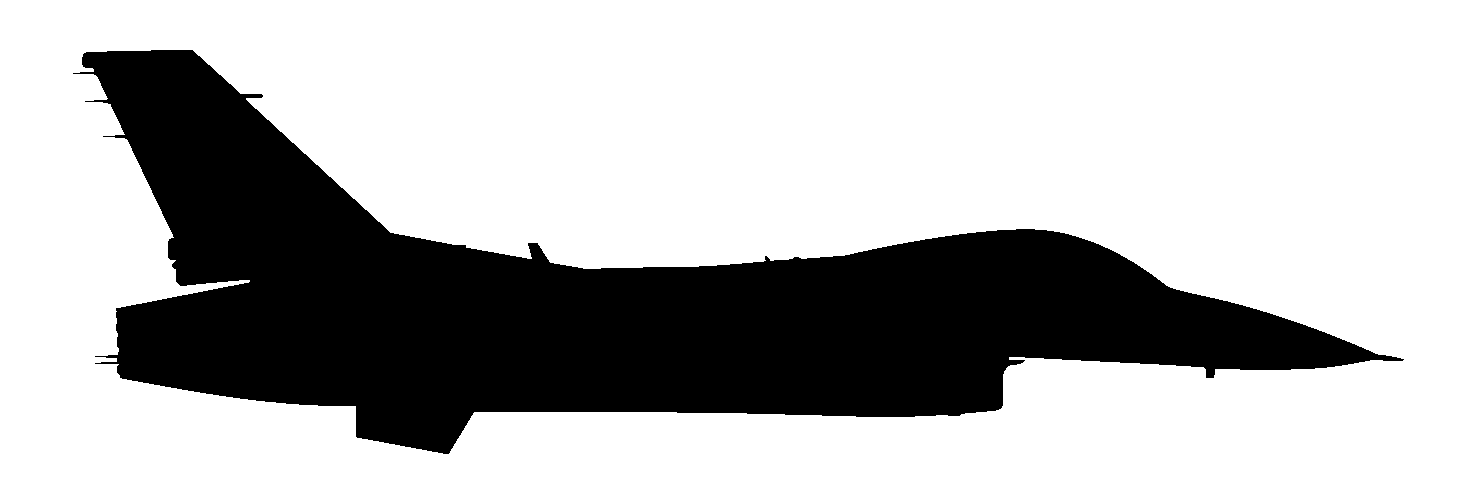
\includegraphics[
                width=12mm,
            ]{diagrams/aircraft/silhouette_f16_side.pdf}
        };
        
        \node[yshift=0.75mm] (4fig) at (4) {
            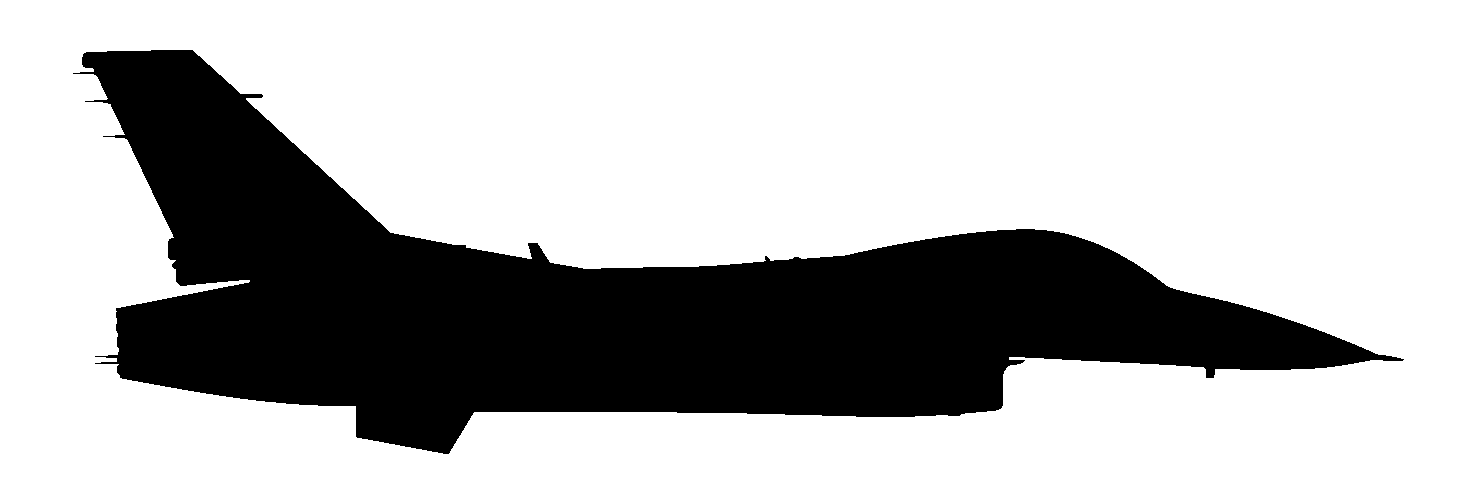
\includegraphics[
                width=12mm,
            ]{diagrams/aircraft/silhouette_f16_side.pdf}
        };

        \node[anchor=north, font=\footnotesize] (1label) at (1fig.west) {1};
        \node[anchor=north, font=\footnotesize] (2label) at (2fig.west) {2};
        \node[anchor=north, font=\footnotesize] (3label) at (3fig.west) {3};
        \node[anchor=north, font=\footnotesize] (4label) at (4fig.west) {4};

    \end{tikzpicture}
    \caption{Stack}
    \label{fig:supp_fig:form:stack}
\end{figure}

\begin{figure}[htbp]
    \centering
    \begin{tikzpicture}[figstyle]
        
        \coordinate (1) at (0,0);
        \coordinate (2) at ($(1)+(-20, 5)$);
        \coordinate (3) at ($(2)+(-20, 5)$);
        \coordinate (4) at ($(3)+(-20, 5)$);

        \draw[<->, thin]
        ($(2)+(10,0)$) 
        -- ($(3)+(30,0)$)
        node[font=\footnotesize, pos=0.5, right] {500-2000 ft};
        \draw[thin]
        (2) -- ($(2)+(12,0)$)
        (3) -- ($(3)+(32,0)$);

        \draw[<->, thin]
        ($(3)+(0,-10)$) 
        -- ($(4)+(0,-15)$)
        node[font=\footnotesize, pos=0.5, below] {0.5-1.0 nm};
        \draw[thin]
        (3) -- ($(3)+(0,-12)$)
        (4) -- ($(4)+(0,-17)$);

        \node[yshift=0.75mm] (1fig) at (1) {
            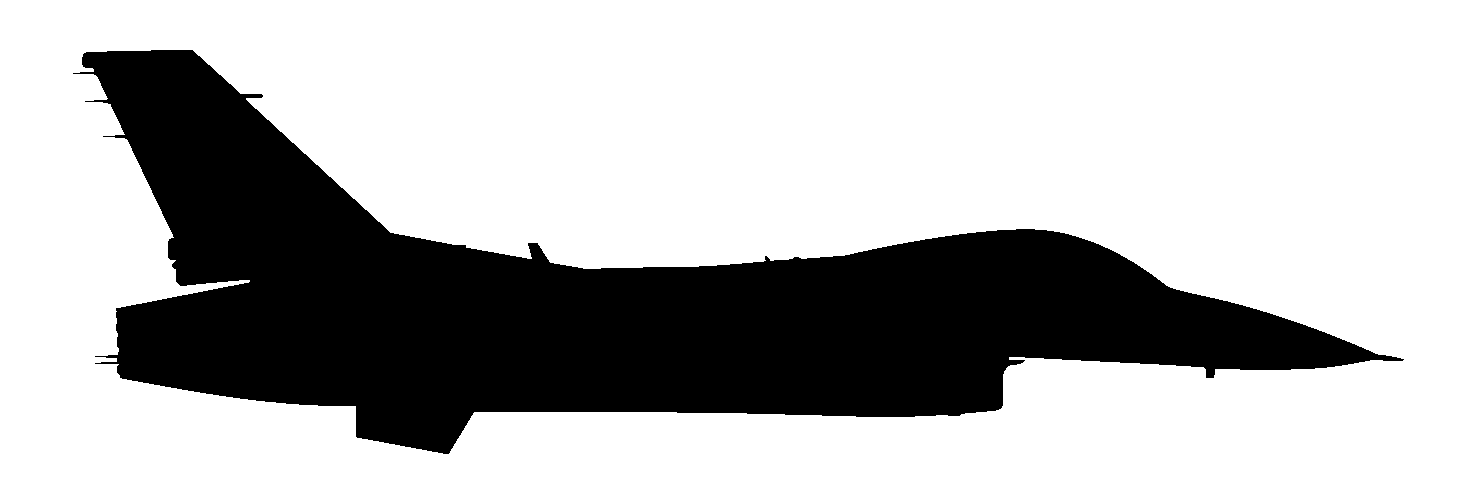
\includegraphics[
                width=12mm,
            ]{diagrams/aircraft/silhouette_f16_side.pdf}
        };
        
        \node[yshift=0.75mm] (2fig) at (2) {
            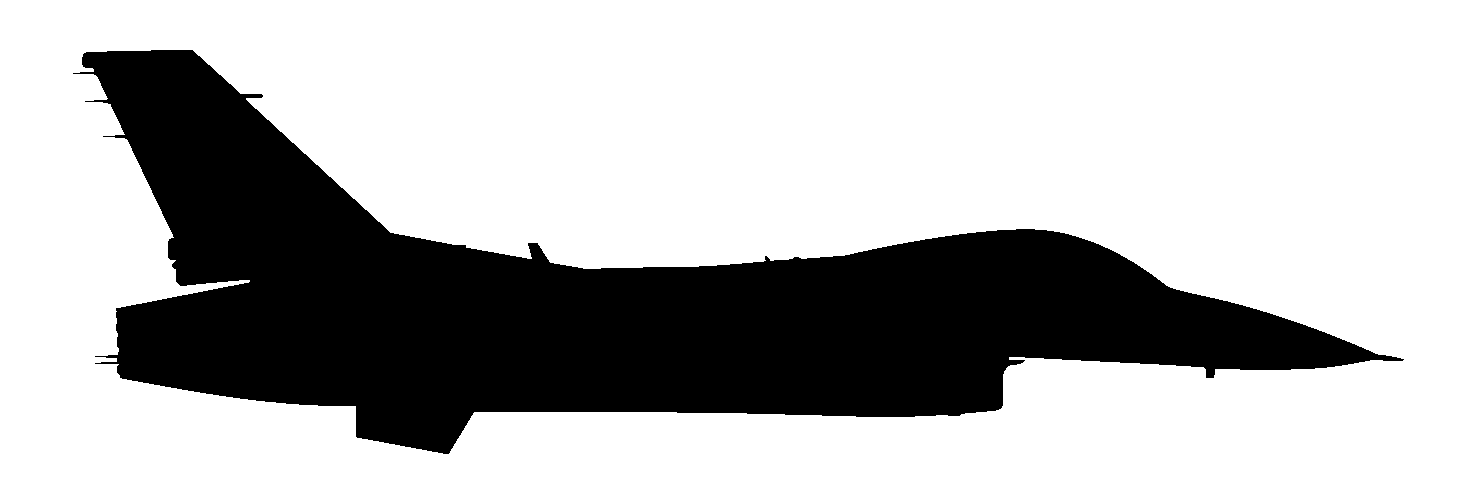
\includegraphics[
                width=12mm,
            ]{diagrams/aircraft/silhouette_f16_side.pdf}
        };

        \node[yshift=0.75mm] (3fig) at (3) {
            \includegraphics[
                width=12mm,
            ]{diagrams/aircraft/silhouette_f16_side.pdf}
        };
        
        \node[yshift=0.75mm] (4fig) at (4) {
            \includegraphics[
                width=12mm,
            ]{diagrams/aircraft/silhouette_f16_side.pdf}
        };

        \node[anchor=north, font=\footnotesize] (1label) at (1fig.west) {1};
        \node[anchor=north, font=\footnotesize] (2label) at (2fig.west) {2};
        \node[anchor=north, font=\footnotesize] (3label) at (3fig.west) {3};
        \node[anchor=north, font=\footnotesize] (4label) at (4fig.west) {4};

    \end{tikzpicture}
    \caption{Ladder}
    \label{fig:supp_fig:form:ladder}
\end{figure}

\clearpage